\documentclass[12pt]{article}
\usepackage{import}
\input{/Users/henrytwiss/Documents/Documents/LaTeX/Notes/Vignettes/preamble.tex}

\title{Modular Forms}
\author{Henry Twiss}
\makeindex

\begin{document}
  \date{}
  \maketitle
  \tableofcontents
  \section{Congruence Subgroups and Modular Curves}
    For any complex \(z\) let
    \[
      e(z) = e^{2\pi iz}.
    \]
    Also, we will distinguish the primitive third root of unity \(\w = e\left(\frac{1}{3}\right)\). All sums and products over a quotient group will be consider to be over a complete set of representatives and we identify cosets with corresponding representatives. If an integer \(a\) is taken modulo \(m\), for any positive integer \(m\), we write \(\conj{a}\) for the inverse of \(a\).
    \subsection{Congruence Subgroups}
      To define congruence subgroups, we first need to introduce an associated group. We call \(\SL_{2}(\Z)\) the \textbf{modular group}\index{modular group} which is the group of matrices with integer entries and of determinant \(1\). We will distinguish two matrices
      \[
        S = \begin{pmatrix} 0 &-1 \\ 1 & 0 \end{pmatrix} \quad \text{and} \quad T = \begin{pmatrix} 1 & 1 \\ 0 & 1 \end{pmatrix}.
      \]
      The first matrix is of order \(4\) while the second has infinite order. The first result usually proved about the modular group is that it is generated by \(S\) and \(T\).

      \begin{proposition}\label{prop:PSL_generator}
          \[
            \SL_{2}(\Z) = \<S,T\>.
          \]
      \end{proposition}
      \begin{proof}
        Let \(n\) be an integer and \(\g = \begin{psmallmatrix} a & b \\ c & d \end{psmallmatrix} \in \SL_{2}(\Z)\). We will prove \(\g \in \<S,T\>\) by demonstrating that it can be reduced to the identity matrix. If \(c = 0\) then \(\g\) is the identity matrix since \(\det(\g) = 1\) and we are done. So suppose \(c \neq 0\) and write \(a = qc+r\) for some integers \(q\) and \(r\) with \(|r| < |c|\). A short computation shows
        \[
          ST^{-q}\g = \begin{pmatrix} -c & -d \\ r & b-qd \end{pmatrix}.
        \]
        The upper-left entry of this matrix strictly larger than the lower-left entry in absolute value. Therefore if we repeatedly apply this argument, it must terminate with the lower-left entry vanishing. But then we have reached the identity matrix.
      \end{proof}
      
      We can now introduce congruence subgroups which are special subgroups of the modular group defined by congruence conditions on their entries. We begin with principal congruence subgroups. For a positive integer \(N\), the \textbf{principal congruence subgroup}\index{principal congruence subgroup} \(\G(N)\) of level \(N\) is defined by
      \[
        \G(N) = \left\{\begin{pmatrix} a & b \\ c & d \end{pmatrix} \in \SL_{2}(\Z):\begin{pmatrix} a & b \\ c & d \end{pmatrix} \equiv \begin{pmatrix} 1 & 0 \\ 0 & 1 \end{pmatrix} \tmod{N}\right\}.
      \]
      This congruence subgroup consists of the matrices which reduce to the identity modulo \(N\). Whence \(\G(N)\) is the kernel of the homomorphism
      \[
        \pi:\SL_{2}(\Z) \to \SL_{2}(\Z/N\Z) \qquad \begin{pmatrix} a & b \\ c & d \end{pmatrix} \mapsto \begin{pmatrix} a & b \\ c & d \end{pmatrix} \pmod{N},
      \]
      and is therefore a normal subgroup. A subgroup \(\G\) of the modular group is said to be a \textbf{congruence subgroup}\index{congruence subgroup} if it contains a principal congruence subgroup. The minimal such \(N\) for which \(\G(N) \subseteq \G\) is called the \textbf{level}\index{level} of \(\G\). Note that if \(M \mid N\) then \(\G(N) \subseteq \G(M)\). Thus if \(\G\) is a congruence subgroup of level \(N\) then it contains the principal congruence subgroups \(\G(kN)\) for all positive integers \(k\). This implies that congruence subgroups are preserved under intersection. In fact, if \(\G_{1}\) and \(\G_{2}\) are congruence subgroups of levels \(N_{1}\) and \(N_{2}\) then \(\G_{1} \cap \G_{2}\) is guaranteed to be a congruence subgroup of level at most \([N_{1},N_{2}]\). Also, it turns out that the aforementioned homomorphism is surjective.

      \begin{proposition}\label{prop:surjective_modulo_N_for_modular_group}
        Let \(N\) be a positive integer. Then the homomorphism
        \[
          \pi:\SL_{2}(\Z) \to \SL_{2}(\Z/N\Z) \qquad \begin{pmatrix} a & b \\ c & d \end{pmatrix} \mapsto \begin{pmatrix} a & b \\ c & d \end{pmatrix} \pmod{N},
        \]
        given by natural projection, is surjective.
      \end{proposition}
      \begin{proof}
        Let \(U\) and \(L\) be the matrices in \(\SL_{2}(\Z/N\Z)\) given by
        \[
          U = \begin{pmatrix} 1 & 1 \\ 0 & 1 \end{pmatrix} \quad \text{and} \quad L = \begin{pmatrix} 1 & 0 \\ 1 & 1 \end{pmatrix}.
        \]
        A short computation shows that these are the images of \(T\) and \(TST\) under \(\pi\) respectively. So \cref{prop:PSL_generator} will imply that \(\pi\) is surjective provided \(U\) and \(L\) generate \(\SL_{2}(\Z/N\Z)\). So let \(\g = \begin{psmallmatrix} a & b \\ c & d \end{psmallmatrix} \in \SL_{2}(\Z/N\Z)\). We will prove \(\g \in \<U,L\>\) by demonstrating that it can be reduced to the identity matrix. To show this, observe that \(U^{n} = U(n)\) and \(L^{n} = L(n)\) where \(U(n)\) and \(L(n)\) are the upper and lower unipotent matrices
        \[
          U(n) = \begin{pmatrix} 1 & n \\ 0 & 1 \end{pmatrix} \quad \text{and} \quad L(n) = \begin{pmatrix} 1 & 0 \\ n & 1 \end{pmatrix},
        \]
        for \(n\) modulo \(N\). So it suffices to show that this collection of unipotent matrices generates \(\SL_{2}(\Z/N\Z)\).  If \(c = 0\) then \(\det(\g) = 1\) implies that \(d = a^{-1}\) so that \(\g = \begin{psmallmatrix} a & b \\ 0 & a^{-1} \end{psmallmatrix}\). Short computations show
        \[
          U(-ab)\g= \begin{pmatrix} a & 0 \\ 0 & a^{-1} \end{pmatrix},
        \]
        and
        \[
          L(a^{-1}-1)U(1)L(a-1)U(-a^{-1}) = \begin{pmatrix} a & 0 \\ 0 & a^{-1} \end{pmatrix}.
        \]
        Whence \(\g\) can be reduced to the identity matrix. If \(c \neq 0\) then \(\det(\g) = 1\) and therefore \(c\) is invertible. A short computation shows
        \[
          L(-c)U((1-a)c^{-1})\g = \begin{pmatrix} 1 & (d-1)c^{-1} \\ 0 & 1 \end{pmatrix},
        \]
        and we recognize this latter matrix is as \(U((d-1)c^{-1})\). Whence \(\g\) can again be reduced to the identity matrix.
      \end{proof}
      
      As \(\G(N)\) is the kernel of this homomorphism, the result implies \([\SL_{2}(\Z):\G(N)] = |\SL_{2}(\Z/N\Z)|\). Since any congruence subgroup \(\G\) contains a principal congruence subgroup of some level, it follows that \(\G\) has finite index in \(\SL_{2}(\Z)\). Accordingly, we set
      \[
        d_{\G} = [\SL_{2}(\Z):\G].
      \]
      We now distinguish two important classes of congruence subgroups other than the principal ones. These are the congruence subgroups
      \[
        \G_{1}(N) = \left\{\begin{pmatrix} a & b \\ c & d \end{pmatrix} \in \SL_{2}(\Z):\begin{pmatrix} a & b \\ c & d \end{pmatrix} \equiv \begin{pmatrix} 1 & \ast \\ 0 & 1 \end{pmatrix} \tmod{N}\right\},
      \]
      and
      \[
        \G_{0}(N) = \left\{\begin{pmatrix} a & b \\ c & d \end{pmatrix} \in \SL_{2}(\Z):\begin{pmatrix} a & b \\ c & d \end{pmatrix} \equiv \begin{pmatrix} \ast & \ast \\ 0 & \ast \end{pmatrix} \tmod{N}\right\},
      \]
      both of which are of level \(N\). These congruence subgroups consist of the matrices which reduce to unipotent upper triangular and upper triangular modulo \(N\) respectively. The latter subgroup \(\G_{0}(N)\) is called the \textbf{Hecke congruence subgroup}\index{Hecke congruence subgroup} of level \(N\). Note that \(\G(N) \subseteq \G_{1}(N) \subseteq \G_{0}(N)\). 
      
      Since the principal congruence subgroups are normal in \(\SL_{2}(\Z)\), if \(\G\) is a congruence subgroup of level \(N\) then so is \(\a^{-1}\G\a\) for any \(\a \in \SL_{2}(\Z)\). In fact, something more general holds. Congruence subgroups are preserved under conjugation by elements of \(\GL_{2}^{+}(\Q)\) provided we restrict to those elements in \(\SL_{2}(\Z)\).

      \begin{lemma}\label{lem:coset_lemma_1}
        Let \(\G\) be a congruence subgroup and \(\a \in \GL_{2}^{+}(\Q)\). Then \(\a^{-1}\G\a \cap \SL_{2}(\Z)\) is a congruence subgroup. In particular, if \(\a^{-1}\G\a \subseteq \SL_{2}(\Z)\) then \(\a^{-1}\G\a\) is a congruence subgroup.
      \end{lemma}
      \begin{proof}
        Let the level of \(\G\) be \(N\) and choose a positive integer \(r\) such that \(r\a,r\a^{-1} \in \GL_{2}^{+}(\Z)\). Let \(M = r^{2}N\) and notice that any \(\g \in \G(M)\) is of the form
        \[
          \g = \begin{pmatrix} 1 & 0 \\ 0 & 1 \end{pmatrix}+M\begin{pmatrix} k_{1} & k_{2} \\ k_{3} & k_{4} \end{pmatrix},
        \]
        for integers \(k_{1},\ldots,k_{4}\). Therefore \(\G(M) \subseteq I+M\Mat_{2}(\Z)\) and so
        \[
          \a\G(M)\a^{-1} \subseteq I+N\Mat_{2}(\Z).
        \]
        As \(\G(N) = (I+N\Mat_{2}(\Z)) \cap \SL_{2}(\Z)\), it follows that \(\a\G(M)\a^{-1} \subseteq \G(N)\). Whence \(\G(M) \subseteq \a^{-1}\G\a\) because \(\G\) is of level \(N\). Intersecting with \(\SL_{2}(\Z)\) proves the first statement. The second statement is immediate.
      \end{proof}

      Note that in the case \(\a^{-1}\G\a \subseteq \SL_{2}(\Z)\), normality of principal congruence subgroups force \(\G\) and \(\a^{-1}\G\a\) to be of the same level. In particular, this will always happen whenever we conjugate by elements of the modular group.
      
      Also, since congruence subgroups are preserved under intersection, the previous lemma further implies that \(\a^{-1}\G_{1}\a \cap \G_{2}\) is a congruence subgroup for any two congruence subgroups \(\G_{1}\) and \(\G_{2}\) and any \(\a \in \GL_{2}^{+}(\Q)\). In this setting, consider the double coset
      \[
        \G_{1}\a\G_{2} = \{\g_{1}\a\g_{2}:\g_{1} \in \G_{1} \text{ and } \g_{2} \in \G_{2}\}.
      \]
      Note that \(\G_{1}\) acts on \(\G_{1}\a\G_{2}\) by left multiplication so that it decomposes into a disjoint union of orbits. That is,
      \[
        \G_{1}\a\G_{2} = \bigcup_{\b \in \G_{1}\backslash\G_{1}\a\G_{2}}\G_{1}\b.
      \]
      It turns out that this union is finite. To see this, we need to relate the orbit space \(\G_{1}\backslash\G_{1}\a\G_{2}\) to a quotient of \(\G_{2}\) with respect to the action of some subgroup. Consider the congruence subgroup \(\a^{-1}\G_{1}\a \cap \G_{2}\) which is a subgroup of \(\G_{2}\). As this subgroup acts on \(\G_{2}\) by left multiplication, we again have an orbit space \((\a^{-1}\G_{1}\a \cap \G_{2})\backslash\G_{2}\). We first show how these orbit spaces are related.

      \begin{lemma}\label{lem:coset_lemma_2}
        Let \(\G_{1}\) and \(\G_{2}\) be congruence subgroups and let \(\a \in \GL_{2}^{+}(\Q)\). Then the right multiplication map
        \[
          \G_{2} \to \G_{1}\backslash\G_{1}\a\G_{2} \qquad \g_{2} \mapsto \G_{1}\a\g_{2},
        \]
        induces a bijection from \((\a^{-1}\G_{1}\a \cap \G_{2})\backslash\G_{2}\) to \(\G_{1}\backslash\G_{1}\a\G_{2}\).
      \end{lemma}
      \begin{proof}
        We first show that this map is \((\a^{-1}\G_{1}\a \cap \G_{2})\)-invariant so that it induces a map on the quotient. Indeed, if \(\g \in \a^{-1}\G_{1}\a \cap \G_{2}\) then \(\g = \a^{-1}\g_{1}\a\) for some \(\g_{1} \in \G_{1}\). Thus \(\G_{1}\a\g\g_{2} = \G_{1}\a\g_{2}\) as claimed. We now show that the induced map is a bijection. 

        We will prove injectivity and then surjectivity. For the former, let \(\g_{2}\) and \(\g'_{2}\) be representatives of orbits of \((\a^{-1}\G_{1}\a \cap \G_{2})\backslash\G_{2}\) such that \(\G_{1}\a\g_{2} = \G_{1}\a\g'_{2}\). This implies \(\a\g_{2}(\g'_{2})^{-1} \in \G_{1}\a\) and so \(\g_{2}(\g'_{2})^{-1} \in \a^{-1}\G_{1}\a\). But we also have \(\g_{2}(\g'_{2})^{-1} \in \G_{2}\) and these two facts together imply that \(\g_{2}(\g'_{2})^{-1} \in \a^{-1}\G_{1}\a \cap \G_{2}\). Hence
        \[
          (\a^{-1}\G_{1}\a \cap \G_{2})\g_{2} = (\a^{-1}\G_{1}\a \cap \G_{2})\g'_{2},
        \]
        from which injectivity follows. For the latter, any representative \(\b\) of an orbit in \(\G_{1}\backslash\G_{1}\a\G_{2}\) is of the form \(\b = \g_{1}\a\g_{2}\) for some \(\g_{1} \in \G_{1}\) and \(\g_{2} \in \G_{2}\). But then \(\g_{2}\) represents an orbit of \((\a^{-1}\G_{1}\a \cap \G_{2})\backslash\G_{2}\) mapping to the orbit represented by \(\b\) as \(\G_{1}\b = \G_{1}\a\g_{2}\). This shows surjectivity.
      \end{proof}

      With this lemma in hand, we can prove that the aforementioned disjoint union is finite.

      \begin{proposition}\label{prop:double_congruence_subgroup_coset_decomposition_is_finite}
        Let \(\G_{1}\) and \(\G_{2}\) be congruence subgroups and let \(\a \in \GL_{2}^{+}(\Q)\). Then the disjoint union
        \[
          \G_{1}\a\G_{2} = \bigcup_{\b \in \G_{1}\backslash\G_{1}\a\G_{2}}\G_{1}\b,
        \]
        is finite.
      \end{proposition}
      \begin{proof}
        By \cref{lem:coset_lemma_2}, the number of orbits of \(\G_{1}\backslash\G_{1}\a\G_{2}\) is in bijection with those of \((\a^{-1}\G_{1}\a \cap \G_{2})\backslash\G_{2}\) which is \([\G_{2}:\a^{-1}\G_{1}\a \cap \G_{2}]\). By \cref{lem:coset_lemma_1}, \(\a^{-1}\G_{1}\a \cap \SL_{2}(\Z)\) is a congruence subgroup and thus \(\a^{-1}\G_{1}\a \cap \G_{2}\) is as well. It follows that \([\G_{2}:\a^{-1}\G_{1}\a \cap \G_{2}] \le d_{\a^{-1}\G_{1}\a \cap \G_{2}}\) where \(d_{\a^{-1}\G_{1}\a \cap \G_{2}}\) is finite which completes the proof.
      \end{proof}
    \subsection{Modular Curves and Fundamental Domains}
      Recall that \(\GL_{2}^{+}(\R)\) acts on the Riemann sphere \(\hat{\C}\) by M\"obius transformations. Explicitly, any \(\a = \begin{psmallmatrix} a & b \\ c & d \end{psmallmatrix} \in \GL_{2}^{+}(\R)\) acts on \(z \in \hat{\C}\) by
      \[
        \a z = \frac{az+b}{cz+d}.
      \]
      Moreover, this group action is invariant under scalar multiplication and negation and acts by automorphisms of \(\hat{\C}\). A short computation shows
      \begin{equation}\label{equ:Mobius_transformation_imaginary_part}
        \Im(\a z) = \det(\a)\frac{\Im(z)}{|cz+d|^{2}},
      \end{equation}
      Therefore \(\a\) preserves the sign of the imaginary part of \(z\) and therefore preserves the upper half-plane \(\H\), the lower half-plane \(\conj{\H}\), and the extended real line \(\hat{\R}\). Whence \(\GL_{2}^{+}(\R)\) acts by automorphisms on these subspaces respectively. In the case of \(\GL_{2}^{+}(\Q)\), we also have a restricted action on \(\hat{\Q}\) by automorphisms since the entries of these matrices are rational. Moreover, if \(\a \in \SL_{2}(\R)\) then we have the simplified relation
      \begin{equation}\label{equ:Mobius_transformation_imaginary_part_simplified}
        \Im(\a z) = \frac{\Im(z)}{|cz+d|^{2}}.
      \end{equation}
      An important restriction of this action is to the modular group \(\SL_{2}(\Z)\). Again, these matrices act on \(\hat{\C}\) by M\"obius transformations and preserves the aforementioned subspaces \(\H\), \(\conj{\H}\), \(\hat{\R}\), and \(\hat{\Q}\) respectively.
      
      We will primarily be interested in certain actions of subgroups of \(\SL_{2}(\R)\) on \(\H\). A \textbf{Fuchsian group}\index{Fuchsian group} is any discrete subgroup of \(\SL_{2}(\R)\) that acts properly discontinuously on \(\H\). The modular group is a prime example of a Fuchsian group.

      \begin{proposition}\label{prop:modular_group_is_Fuchsian}
        The modular group is a Fuchsian group.
      \end{proposition}
      \begin{proof}
        \(\SL_{2}(\Z)\) is discrete in \(\SL_{2}(\R)\) because \(\Z\) is discrete in \(\R\). So it remains to show that \(\SL_{2}(\Z)\) acts properly discontinuously on \(\H\). To prove this, it suffices to show that for any compact subset \(K \subset \H\) there are finitely many \(\g = \begin{psmallmatrix} a & b \\ c & d \end{psmallmatrix} \in \SL_{2}(\Z)\) satisfying \(\g K \cap K \neq 0\). Set \(M = \min_{z \in K}\Im(z)\). If \(\g K \cap K \neq \emt\) then there exists a \(z \in K\) such that \(\Im(\g z) \ge M\). This inequality is equivalent to
        \[
          (cx+d)^{2}+(cy)^{2} \le \frac{y}{M},
        \]
        by \cref{equ:Mobius_transformation_imaginary_part_simplified}, which is only satisfied for finitely many pairs of relatively prime integers \((c,d)\) since \(y > 0\). Each pair determines infinitely many matrices \(\g_{k} = \begin{psmallmatrix} a+kc & b+kd \\ c & d \end{psmallmatrix} \in \SL_{2}(\Z)\) possibly satisfying \(\g_{k}K \cap K \neq \emt\). As \(K\) is compact it has bounded real part and so only finitely many such \(k\) satisfy this condition. Hence there are finitely many possible matrices \(\g\).
      \end{proof}
      
      As an immediate consequence of this result, any subgroup of the modular group is also Fuchsian. In particular, all congruence subgroups are Fuchsian. Fuchsian groups are important because proper discontinuity of the group action ensures that the corresponding quotient of \(\H\) wil be connected Hausdorff because \(\H\) is. The principal example of such quotients are modular curves.
      
      A \textbf{modular curve}\index{modular curve} is a quotient \(\GH\) of the upper half-plane \(\H\) by the action of a congruence subgroup \(\G\). Then, as remarked before, \(\GH\) is connected Hausdorff because \(\G\) is Fuchsian. In particular, \(\GH\) admits a fundamental domain
      \[
        \mc{F} = \left\{z \in \H:|\Re(z)| \le \frac{1}{2} \text{ and } |z| \ge 1\right\},
      \]
      as the following proposition shows:

      \begin{proposition}\label{prop:fundamental_domain_modular_group}
        \(\mc{F}\) is a fundamental domain for the modular group.
      \end{proposition}
      \begin{proof}
        We first show any point in \(\H\) is \(\SL_{2}(\Z)\)-equivalent to a point in \(\mc{F}\). So let \(z \in \H\) and \(\g = \begin{psmallmatrix} a & b \\ c & d \end{psmallmatrix} \in \SL_{2}(\Z)\). Then \cref{equ:Mobius_transformation_imaginary_part_simplified} gives
        \[
          \Im(\g z) = \frac{y}{|cz+d|^{2}}.
        \]
        Since \(\det(\g) = 1\) we cannot have \(c = d = 0\). As \(y > 0\), it is easily checked that \(|cz+d| \ge \min(y,1)\) and thus bounded away from zero. Whence there are finitely many pairs of relatively prime integers \((c,d)\) such that \(|cz+d|^{2} \le M\) for any \(M > 0\). So choose a \(\g\) such that it minimizes \(|cz+d|\) and hence maximizes \(\Im(\g z)\). In particular, \(\Im(S\g z) \le \Im(\g z)\) which is to say
        \[
          \frac{\Im(\g z)}{|\g z|^{2}} \le \Im(\g z).
        \]
        The inequality implies \(|\g z| \ge 1\). Since \(\Im(T^{n}\g z) = \Im(\g z)\) for all integers \(n\), repeating the argument above with \(T^{n}\g\) in place of \(\g\), we see that \(|T^{n}\g z| \ge 1\). But \(T\) shifts the real part by \(1\) so we can choose \(n\) such that \(|\Re(T^{n}\g z)| \le \frac{1}{2}\). Therefore \(T^{n}\g\) maps \(z\) into \(\mc{F}\). It remains to show that no two distinct interior points of \(\mc{F}\) are \(\SL_{2}(\Z)\)-equivalent. So suppose to the contrary that there exist distinct \(z,z' \in \mc{F}^{\circ}\) and \(\g \in \SL_{2}(\Z)\) such that \(z' = \g z\). Without loss of generality, we may assume \(\Im(z') \ge \Im(z)\). Then
        \[
          \Im(z') = \frac{\Im(z)}{|cz+d|^{2}},
        \]
        by \cref{equ:Mobius_transformation_imaginary_part_simplified} and so \(|cz+d| \le 1\). As \(|z| > 1\) and \(|\Re(z)| < \frac{1}{2}\), short computations show that this inequality is valid only if \(c = 0\). Then \(\det(\g) = 1\) forces \(a = d = \pm 1\). Finally, \(|\Re(z)| < \frac{1}{2}\) further forces \(b = 0\). But then \(\g = \pm I\) which gives a contradiction since we assumed \(z\) and \(z'\) were distinct.
      \end{proof}

      \begin{figure}[ht]
        \centering
        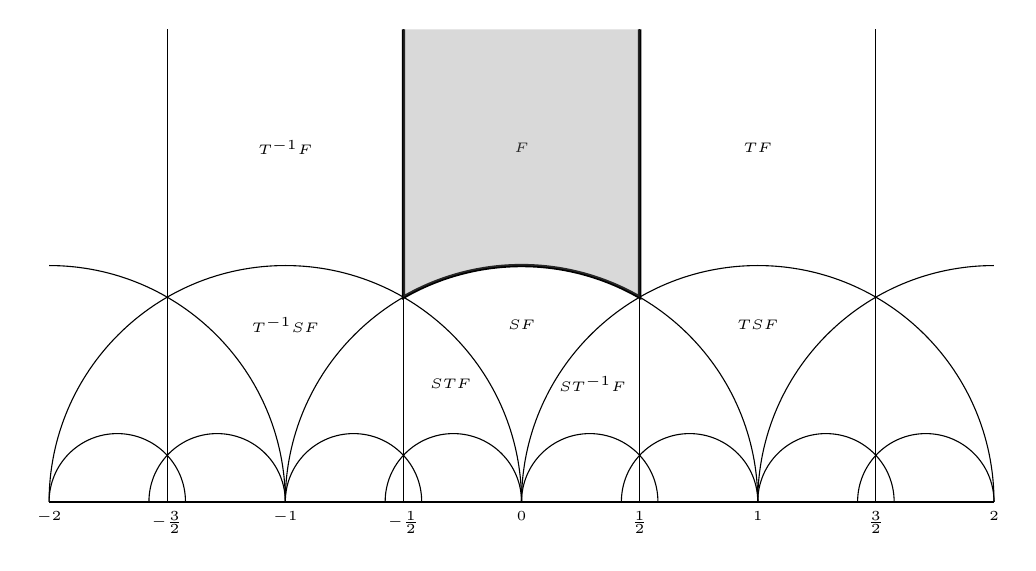
\begin{tikzpicture}[scale=3]
          \def\xmin{-2} \def\xmax{2}
          \def\ymin{0} \def\ymax{2}
          \draw[thick] (\xmin,0) -- (\xmax,0);

          \draw[very thick] (0.5,\ymax) -- (0.5,{sqrt(3)/2}) arc (60:120:1) -- (-0.5,\ymax);

          \node at (-0.5,0) [below] {\tiny{\(-\frac{1}{2}\)}};
          \node at (0.5,0) [below] {\tiny{\(\frac{1}{2}\)}};
          \node at (-1.5,0) [below] {\tiny{\(-\frac{3}{2}\)}};
          \node at (1.5,0) [below] {\tiny{\(\frac{3}{2}\)}};
          \node at (0,0) [below] {\tiny{\(0\)}};
          \node at (-1,0) [below] {\tiny{\(-1\)}};
          \node at (1,0) [below] {\tiny{\(1\)}};
          \node at (-2,0) [below] {\tiny{\(-2\)}};
          \node at (2,0) [below] {\tiny{\(2\)}};

          \draw[thin] (0.5,0) -- (0.5,\ymax);
          \draw[thin] (-0.5,0) -- (-0.5,\ymax);
          \draw[thin] (1.5,0) -- (1.5,\ymax);
          \draw[thin] (-1.5,0) -- (-1.5,\ymax);

          \draw (1,0) arc (0:180:1);
          \draw (-1,0) arc (0:90:1);
          \draw (2,1) arc (90:180:1);

          \draw (0,0) arc (0:180:1);
          \draw (2,0) arc (0:180:1);

          \draw (1,0) arc (0:180:{sqrt(3)/6});
          \draw ({sqrt(3)/3},0) arc (0:180:{sqrt(3)/6});

          \draw (2,0) arc (0:180:{sqrt(3)/6});
          \draw ({1+sqrt(3)/3},0) arc (0:180:{sqrt(3)/6});

          \draw (0,0) arc (0:180:{sqrt(3)/6});
          \draw ({(sqrt(3)/3)-1},0) arc (0:180:{sqrt(3)/6});

          \draw (-1,0) arc (0:180:{sqrt(3)/6});
          \draw ({(sqrt(3)/3)-2},0) arc (0:180:{sqrt(3)/6});

          \node at (0,1.5) {\tiny{\(\mc{F}\)}};
          \node at (-1,1.5) {\tiny{\(T^{-1}\mc{F}\)}};
          \node at (1,1.5) {\tiny{\(T\mc{F}\)}};
          \node at (0,0.75) {\tiny{\(S\mc{F}\)}};
          \node at (-1,0.75) {\tiny{\(T^{-1}S\mc{F}\)}};
          \node at (1,0.75) {\tiny{\(TS\mc{F}\)}};
          \node at (-0.3,0.5) {\tiny{\(ST\mc{F}\)}};
          \node at (0.3,0.5) {\tiny{\(ST^{-1}\mc{F}\)}};

          \begin{scope}
            \path[clip] (0.5,\ymax) -- (0.5,{sqrt(3)/2}) arc (60:120:1) -- (-0.5,\ymax) -- cycle;
            \fill[gray,opacity=0.3] (-0.5,0) rectangle (0.5,\ymax);
          \end{scope}
        \end{tikzpicture}
        \caption{The standard fundamental domain for \(\SL_{2}(\Z)\backslash\H\).} \label{fig:fundamental_domain_modular_group}
      \end{figure}
      
      The region \(\mc{F}\), shaded in \cref{fig:fundamental_domain_modular_group}, is called the \textbf{standard fundamental domain}\index{standard fundamental domain}. This figure also displays how this fundamental domain changes under the actions of the generators of \(\SL_{2}(\Z)\) as in \cref{prop:PSL_generator}.

      \begin{remark}\label{rem:vertices_of_standard_fundamental_domain}
        Any \(z \in \mc{F}\) satisfies \(\Im(z) \ge \frac{\sqrt{3}}{2}\). Indeed, any \(z \in \mc{F}\) occurs on the arc of a circle of radius \(r \ge 1\) subject to \(|\Re(z)| \le \frac{1}{2}\). Then \(\Im(z)\) is minimized on the arc \(|z| = 1\), and on this arc
        \[
          \Im(z) = \sqrt{1-\Re(z)^{2}}.
        \]
        The right-hand side is minimized at \(\Re(z) = \pm\frac{1}{2}\) giving \(\Im(z) = \frac{\sqrt{3}}{2}\). This corresponds to the points \(-\frac{1}{2}+i\frac{\sqrt{3}}{2}\) and \(\frac{1}{2}+i\frac{\sqrt{3}}{2}\) which are \(\w\) and \(1+\w\) respectively. They are the vertices of the boundary of \(\mc{F}\).
      \end{remark}
    
      Any other modular curve \(\GH\) admits a fundamental domain
      \[
        \mc{F}_{\G} = \bigcup_{\g \in \G\backslash\SL_{2}(\Z)}\g\mc{F},
      \] 
      obtained from the standard fundamental domain using representatives of orbits of \(\G\backslash\SL_{2}(\Z)\) as the following proposition shows:

      \begin{proposition}\label{prop:fundamental_domain_congruence_subgroup}
        Let \(\G\) be a congruence subgroup. Then \(\mc{F}_{\G}\) is a fundamental domain for \(\G\backslash\H\).
      \end{proposition}
      \begin{proof}
        We first show that every point in \(\H\) is \(\G\)-equivalent to a point in \(\mc{F}_{\G}\). From the definition of \(\mc{F}_{\G}\), it is straightforward to check that
        \[
          \bigcup_{\g' \in \G}\g'\mc{F}_{\G} = \H.
        \]
        Whence every point in \(\H\) is \(\G\)-equivalent to a point in \(\mc{F}_{\G}\). We will now show that no two distinct interior points of \(\mc{F}_{\G}\) are \(\G\)-equivalent. Suppose to the contrary that there are distinct \(z_{1},z_{2} \in \mc{F}_{\G}^{\circ}\) and a \(\g \in \G\) such that \(\g z_{1} = z_{2}\). In particular, \(z_{1} \in \g_{1}\mc{F}^{\circ}\) and \(z_{2} \in \g_{2}\mc{F}^{\circ}\) for some \(\g_{1},\g_{2} \in \G\backslash\SL_{2}(\Z)\). As no two distinct interior points of \(\mc{F}\) are \(\SL_{2}(\Z)\)-equivalent, this forces \(\g_{1}\) and \(\g_{2}\) to belong to the same coset of \(\G\backslash\SL_{2}(\Z)\). Whence \(\g_{1} = \g_{2}\) and implying \(z_{1},z_{2} \in \g_{1}\mc{F}^{\circ} \cap \g_{2}\mc{F}^{\circ}\). This gives a contradiction since no two distinct interior points of \(\mc{F}\) are \(\SL_{2}(\Z)\)-equivalent. Hence no two distinct interior points of \(\mc{F}_{\G}\) are \(\G\)-equivalent.
      \end{proof}

      It is also possible to say something about the stabilizer subgroups of points in \(\H\) with respect to the action of a congruence subgroup \(\G\). Let \(\G_{z}\) denote the stabilizer subgroup of \(z \in \H\). Then \(\G_{\g z} = \g\G_{z}\g^{-1}\) for any \(\g \in \G\) and it follows that all of the stabilizer subgroups are determined by those for \(z \in \mc{F}_{\G}\). Moreover, since \(\mc{F}_{\G}\) is a fundamental domain, \(\G_{z}\) is trivial if \(z \in \mc{F}_{\G}^{\circ}\). So any point with a nontrivial stabilizer subgroups must lie on the boundary of \(\mc{F}_{\G}\). As \(\G\) is a subgroup of \(\SL_{2}(\Z)\), \(\G_{z}\) is a subgroup of \((\SL_{2}(\Z))_{z}\). This leads us to determining the stabilizer subgroups in the case of the modular group.

      \begin{proposition}\label{prop:stabilizer_subgroup}
        Let \(z \in \mc{F}\). Then
        \[
          (\SL_{2}(\Z))_{z} = \begin{cases} \<S\> & \text{if \(z = i\)}, \\ \<ST\> & \text{if \(z = \w\)}, \\ \<TS\> & \text{if \(z = 1+\w\)}, \\ \<-I\> & \text{if \(z \neq i,\w,1+\w\)}. \end{cases}
        \]
        Moreover, \((\SL_{2}(\Z))_{i}\) is of order \(4\) while \((\SL_{2}(\Z))_{\w}\) and \((\SL_{2}(\Z))_{1+\w}\) are of order \(6\).
      \end{proposition}
      \begin{proof}
        Let \(\g = \begin{psmallmatrix} a & b \\ c & d \end{psmallmatrix} \in \SL_{2}(\Z)\). Then \(\g z = z\) implies
        \[
          cz^{2}+(d-a)z-b = 0.
        \]
        We will analyze this identity on a case by case basis. In particular, we will take \(z = i\), \(z = \w\), \(z = 1+\w\), and \(z \neq i,\w,1+\w\) respectively.

        Taking \(z = i\) in this identity gives
        \[
          -c+(d-a)i-b = 0.
        \]
        Equating the real and imaginary parts shows that \(b = -c\) and \(d = a\). Then \(\g = \begin{psmallmatrix} a & -c \\ c & a \end{psmallmatrix}\) and \(a^{2}+c^{2} = 1\). Therefore we have \(a = 1\) and \(c = 0\), \(a = -1\) and \(c = 0\), \(a = 0\) and \(c = 1\), or \(a = 0\) and \(c = -1\). These four cases correspond to the matrices \(I\), \(-I\), \(S\), and \(-S\) respectively. Since \(S^{2} = -I\), it follows that \((\SL_{2}(\Z))_{i} = \<S\>\) and is of order \(4\).
        
        Taking \(z = \w\) in the identity instead gives
        \[
          c\w^{2}+(d-a)\w-b = 0.
        \]
        Recall that \(m_{\w}(x) = x^{2}+x+1\) is the minimal polynomial for \(\w\) over \(\Q\). So \(\w^{2} = -\w-1\) and substituting this identity into the one above yields
        \[
        (d-a-c)\w-(b+c) = 0.
        \]
        By minimality of \(m_{\w}(x)\), \(\w\) and \(1\) are linearly independent over \(\Q\) so we may equate coefficients to see that \(d = a+c\) and \(b = -c\). Then \(\g = \begin{psmallmatrix} a & -c \\ c & a+c \end{psmallmatrix}\) and \(a^{2}+ac+c^{2} = 1\). Completing the square shows \((a+c)^{2}-ac = 1\). Therefore we have \(a = 1\) and \(c = 0\), \(a = -1\) and \(c = 0\), \(a = 0\) and \(c = 1\), \(a = 0\) and \(c = -1\), \(a = -1\) and \(c = 1\), or \(a = 1\) and \(c = -1\). These six cases correspond to the matrices \(I\), \(-I\), \(ST\), \((ST)^{4}\), \((ST)^{2}\), and \((ST)^{5}\) respectively. As \((ST)^{3} = -I\), it follows that \((\SL_{2}(\Z))_{\w} = \<ST\>\) and is of order \(6\). Moreover, if \(z = 1+\w\) then \(z = T\w\). Whence \((\SL_{2}(\Z))_{1+\w} = T(\SL_{2}(\Z))_{\w}T^{-1} = \<TS\>\) and is of order \(6\).
        
        It remains to show that if \(z \neq i,\w,1+\w\) then \((\SL_{2}(\Z))_{z} = \<I\>\). Equivalently, will show the contrapositive which is to say that if \((\SL_{2}(\Z))_{z} \neq \<-I\>\) then \(z = i,\w,1+\w\). Since the stabilizer subgroup of \(z\) is trivial if \(z \in \mc{F}^{\circ}\), we may additionally assume \(z\) lies on the boundary of \(\mc{F}\). Now suppose for such \(z\) that \(\g \neq \pm I\). We first claim \(c > 0\). For if \(c = 0\), \(\det(\g) = 1\) implies \(a = d = \pm1\). This further forces \(b = 0\) implying \(\g = \pm I\) which is a contradiction. Hence \(c \neq 0\) and so \(z\) satisfies the aforementioned identity which is a quadratic. A short computation shows that the discriminant is \((a+d)^{2}-4\). Since this quadratic has integer coefficients and \(z\) is complex, the discriminant must be negative. So
        \[
          (a+d)^{2}-4 < 0,
        \]
        which forces \(a+d = 0,1,-1\). These three cases correspond to the discriminant being \(-4\) in the first case and \(-3\) in the latter two cases. Whence the quadratic formula implies
        \[
          z = \frac{a\pm i}{c}, \quad \text{or} \quad z = \frac{2a-1\pm\sqrt{3}i}{2c}, \quad \text{or} \quad z = \frac{2a+1\pm\sqrt{3}i}{2c},
        \]
        respectively. In any case, the bound \(\Im(z) \ge \frac{\sqrt{3}}{2}\) by \cref{rem:vertices_of_standard_fundamental_domain} implies \(c = \pm 1\). This forces \(a = 0\) in the first case, \(a = 0,1\) in the second, and \(a = 0,-1\) in the third. Whence \(z = i\) in the first case and \(z = \w,1+\w\) in the second and third cases. This completes the proof.
      \end{proof}

      Returning to the case of a congruence subgroup \(\G\), it follows from this result and our previous remarks that \(\G_{z}\) is necessarily trivial if \(z\) is not \(\SL_{2}(\Z)\)-equivalent to \(i\), \(\w\), or \(1+\w\). Moreover, if \(z\) is \(\SL_{2}(\Z)\)-equivalent to one of these points then \(\G_{z}\) is trivial unless at least one of the matrices \(\pm S\), \(\pm ST\), or \(\pm TS\) belongs to \(\G\) respectively. In the the first case \(\G_{z}\) is of order dividing \(4\) while in the second and third cases it is of order dividing \(6\). In particular, \(\G_{z}\) is always finite.
    \subsection{Cusps}
      Let \(\G\) be a congruence subgroup. Notice that \(\mc{F}_{\G}\) is not compact as it doesn't contain any points of \(\hat{\Q}\). However, if we consider \(\mc{F}_{\G} \cup \hat{\Q}\) as a subset of \(\hat{\C}\) then it would appear that this space is compact. The elements of \(\hat{\Q}\) correspond to cusps which we now define. Really that any \(\g \in \G\) acts on \(\hat{\Q}\). A \textbf{cusp class}\index{cusp class} of \(\GH\) is a coset of \(\G\backslash\hat{\Q}\). There is only one cusp class for the modular group since its action is transitive. Indeed, \(\hat{\Q}\) is exactly the orbit of \(\infty\). This is clear for \(\infty\) and if \(\frac{a}{c} \in \Q\) with \((a,c) = 1\) then B\'ezout's identity provides the existence of integers \(b\) and \(d\) such that \(ad-bc = 1\) whence \(\g = \begin{psmallmatrix} a & b \\ c & d \end{psmallmatrix} \in \SL_{2}(\Z)\) satisfies \(\g\infty = \frac{a}{c}\). Therefore the action is transitive. As \(\G\) has finite index in the modular group and \(\hat{\Q} = \SL_{2}(\Z)\infty\), there can only be finitely many cosets of \(\G\backslash\hat{\Q}\) and the number of such is at most \(d_{\G}\). In other words, \(\GH\) has at most \(d_{\G}\) cusp classes. Also, the orbit of \(\infty\) is a cusp class of \(\GH\). A \textbf{cusp}\index{cusp} is a representative of a cusp class. We denote cusps by gothic characters \(\mf{a}\), \(\mf{b}\), etc.

      \begin{remark}
        The cusps are exactly the points needed to make a fundamental domain \(\mc{F}_{\G}\) compact as a subset of \(\hat{\C}\). To see this, suppose \(\mf{a}\) is a limit point of \(\mc{F}_{\G}\) that does not belong to \(\mc{F}_{\G}\). Then \(\mf{a} \in \hat{\R}\). As the unique limit point of \(\mc{F}\) not belonging to \(\mc{F}\) is \(\infty\) and \(\hat{\Q} = \SL_{2}(\Z)\infty\), \cref{prop:fundamental_domain_congruence_subgroup} implies \(\mf{a} \in \hat{\Q}\) which means \(\mf{a}\) is a cusp. In the case of the standard fundamental domain \(\mc{F}\), the only cusp is \(\infty\).
      \end{remark}

      We will now describe the stabilizer subgroups of \(\G\) relative to a cusp \(\mf{a}\). This will slightly depend upon if \(\G\) contains \(-I\), so let \(\e_{\G} = 1,0\) according to if \(-I \in \G\) or not. We will denote the stabilizer subgroup of the cusp \(\mf{a}\) by \(\G_{\mf{a}}\). We begin by describing \(\G_{\infty}\). For if \(\g = \begin{psmallmatrix} a & b \\ c & d \end{psmallmatrix} \in \G\) stabilizes \(\infty\) then necessarily \(c = 0\) and since \(\det(\g) = 1\) we must have \(a = d = \pm 1\) or \(a = d = 1\) according to if \(-I \in \G\) or not. In either case, \(\g\) acts on \(\H\) by translation by \(b\). If we let \(h_{\infty}\) be the smallest positive integer such that \(\g_{\infty} = \begin{psmallmatrix} 1 & h_{\infty} \\ 0 & 1 \end{psmallmatrix} \in \G_{\infty}\) then
      \[
        \G_{\infty} = \<\g_{\infty},(-I)^{\e_{\G}}\>.
      \]
      By our previous discussion, there exists a matrix \(\s_{\mf{a}} \in \SL_{2}(\Z)\) such that \(\s_{\mf{a}}\infty = \mf{a}\). We call \(\s_{\mf{a}}\) a \textbf{scaling matrix}\index{scaling matrix} for \(\mf{a}\). Note that \(\s_{\mf{a}}\) is determined up to composition on the right by an element of \(\G_{\infty}\). If \(\mf{a} = \infty\) then we may take \(\s_{\mf{a}} = I\) and in this case we suppress the dependence upon the scaling matrix. Scaling matrices are useful because they allow us to transfer information at the cusp \(\mf{a}\) to the cusp at \(\infty\). We will use them to determine the stabilizer subgroups of other cusps. If \(\s_{\mf{a}}\) is a scaling matrix for the cusp \(\mf{a}\) then \(\G_{\mf{a}} = \s_{\mf{a}}\G_{\infty}\s_{\mf{a}}^{-1} \cap \G\). Whence
      \[
        \G_{\mf{a}} = \<\g_{\mf{a}},(-I)^{\e_{\G}}\>,
      \]
      where \(\g_{\mf{a}}\) is of the form
      \[
        \g_{\mf{a}} = \s_{\mf{a}}\begin{pmatrix} 1 & h_{\mf{a}} \\ 0 & 1 \end{pmatrix}\s_{\mf{a}}^{-1},
      \]
      for some positive integer \(h_{\mf{a}}\). We call \(h_{\mf{a}}\) the \textbf{width}\index{width} of the cusp \(\mf{a}\). Equivalently, \(h_{\mf{a}}\) is the shift of the minimal translation belonging to \(\s_{\mf{a}}^{-1}\G\s_{\mf{a}}\). Also observe that \(h_{\mf{a}}\) does not depend on the choice of scaling matrix. We will set
      \[
        \g_{\infty}^{(h_{\mf{a}})} = \begin{pmatrix} 1 & h_{\mf{a}} \\ 0 & 1 \end{pmatrix} \quad \text{and} \quad \G_{\infty}^{(h_{\mf{a}})} = \<\g_{\infty}^{(h_{\mf{a}})},(-I)^{\e_{\G}}\>,
      \]
      so that
      \[
        \G_{\mf{a}} = \s_{\mf{a}}\G_{\infty}^{(h_{\mf{a}})}\s_{\mf{a}}^{-1}.
      \]
      In particular, \(\g_{\infty}^{(h_{\infty})} = \g_{\infty}\) and \(\G_{\infty}^{(h_{\infty})} = \G_{\infty}\).

      \begin{remark}\label{rem:scaling_matrix_to_cusp_class}
        Suppose \(\mf{a}'\) is a cusp that belongs to the same cusp class at \(\mf{a}\). Then \(\mf{a}' = \g\mf{a}\) for some \(\g \in \G\). It follows that \(\g\s_{\mf{a}}\) is a scaling matrix for the cusp \(\mf{a}'\). So \(\G\s_{\mf{a}}\G_{\infty}\) only depends upon the cusp class of \(\mf{a}\) which is \(\G\s_{\mf{a}}\infty\). Moreover, it is easy to see that \(\G_{\mf{a}'} = \g\G_{\mf{a}}\g^{-1}\) and \(\G_{\mf{a}'} = \g\s_{\mf{a}}\G_{\infty}\s_{\mf{a}}^{-1}\g^{-1} \cap \G\). Whence \(\g_{\mf{a}'} = \g\g_{\mf{a}}\g^{-1}\) and therefore \(h_{\mf{a}} = h_{\mf{a'}}\) because the width of a cusp does not depend upon the choice of scaling matrix. This means that the width of \(\mf{a}\) only depends upon its cusp class and so the same is true for \(\g_{\infty}^{(h_{\mf{a}})}\) and \(\G_{\infty}^{(h_{\mf{a}})}\).
      \end{remark}
      
       If \(\G\) is of level \(N\) then \(N\) is the smallest positive integer such that \(\G(N) \subseteq \G\). This means \(\begin{psmallmatrix} 1 & N \\ 0 & 1 \end{psmallmatrix}\) is the minimal translation guaranteed to belong to \(\G\). Since principal congruence subgroups are normal in the modular group, we have \(\G(N) \subseteq \G_{\infty}^{(h_{\mf{a}})}\) and so the aforementioned translation must be a power of \(\g_{\mf{a}}\) which means \(h_{\mf{a}} \mid N\).
       
       We say \(\G\) is \textbf{reduced}\index{reduced} at \(\mf{a}\) if \(h_{\mf{a}} = 1\). For example, the congruence subgroups \(\G_{0}(N)\), \(\G_{1}(N)\), and \(\G(N)\) are all reduced at \(\infty\). The width of the cusps are also related to the index \(d_{\G}\) in a simple manner.

      \begin{proposition}\label{prop:sum_of_widths_equals_index}
        For any congruence subgroup \(\G\) and any cusp \(\mf{a}\) of \(\GH\), there are \(h_{\mf{a}}\) many cosets of \(\G\backslash\SL_{2}(\Z)\) whose elements are scaling matrices for cusps in the cusp class of \(\mf{a}\). In particular,
        \[
          \sum_{\mf{a} \in \G\backslash\hat{\Q}}h_{\mf{a}} = d_{\G}.
        \]
      \end{proposition}
      \begin{proof}
        Let \(\s_{\mf{a}}\) be a scaling matrix for a cusp \(\mf{a}\). It follows from \cref{rem:scaling_matrix_to_cusp_class} that the cusp classes of \(\GH\) are in bijection with the double cosets of \(\G\backslash\SL_{2}(\Z)/\G_{\infty}\) where a cusp class \(\G\s_{\mf{a}}\infty\) corresponds to the double coset \(\G\s_{\mf{a}}\G_{\infty}\) under this bijection. As every element of \(\SL_{2}(\Z)\) is a scaling matrix for some cusp, consider the surjection
        \[
          \phi:\G\backslash\SL_{2}(\Z) \to \G\backslash\SL_{2}(\Z)/\G_{\infty} \qquad \G\s_{\mf{a}} \mapsto \G\s_{\mf{a}}\G_{\infty}.
        \]
        We will compute the number of cosets in a fiber of \(\phi\). Suppose \(\mf{a}\) and \(\mf{a}'\) are representatives of the same cusp class so that \(\G\s_{\mf{a}}\) and \(\G\s_{\mf{a}'}\) belong to the fiber of \(\G\s_{\mf{a}}\G_{\infty} = \G\s_{\mf{a}'}\G_{\infty}\). Then \(\s_{\mf{a}'} = \g\s_{\mf{a}}\g_{\infty}^{n}\) for some \(\g \in \G\) and integer \(n\). Whence \(\G\s_{\mf{a}} = \G\s_{\mf{a}'}\) if and only if \(\G\s_{\mf{a}} =  \G\s_{\mf{a}}\g_{\infty}^{n}\) which is to say that \(\g_{\infty}^{n} \in \s_{\mf{a}}^{-1}\G\s_{\mf{a}}\). As \(\g_{\infty}^{n} \in \G_{\infty}\), this latter condition is further equivalent to \(\g_{\infty}^{n} \in \s_{\mf{a}}^{-1}\G\s_{\mf{a}} \cap \G_{\infty} = \s_{\mf{a}}^{-1}\G_{\mf{a}}\s_{\mf{a}} = \G_{\infty}^{(h_{\mf{a}})}\) which happens if and only if \(h_{\mf{a}} \mid n\). So the cosets \(\G\s_{\mf{a}}\) and \(\G\s_{\mf{a}'}\) are equal if and only if \(h_{\mf{a}} \mid n\). This means there are \(h_{\mf{a}}\) cosets in the fiber of \(\G\s_{\mf{a}}\G_{\infty}\). In other words, there are \(h_{\mf{a}}\) many cosets of \(\G\backslash\SL_{2}(\Z)\) whose elements are scaling matrices for cusps in the cusp class of \(\mf{a}\). This proves the first statement. For the second, the sum of the number of cosets in the fibers of \(\phi\) is equal to the order of \(\G\backslash\SL_{2}(\Z)\) since \(\phi\) is surjective. But this means
        \[
          \sum_{\mf{a} \in \G\backslash\hat{\Q}}h_{\mf{a}} = d_{\G},
        \]
        proving the second statement.
      \end{proof}
      
      Let \(\mf{a}\) and \(\mf{b}\) be cusps of \(\GH\) with scaling matrices \(\s_{\mf{a}}\) and \(\s_{\mf{b}}\) respectively. It will be essential to have a double coset decomposition for sets of the form \(\s_{\mf{a}}^{-1}\G\s_{\mf{b}}\). This is known as the \textbf{Bruhat decomposition}\index{Bruhat decomposition} for \(\s_{\mf{a}}^{-1}\G\s_{\mf{b}}\).

      \begin{theorem*}[Bruhat decomposition]
        Let \(\G\) be a congruence subgroup and let \(\mf{a}\) and \(\mf{b}\) be cusps of \(\GH\) with scaling matrices \(\s_{\mf{a}}\) and \(\s_{\mf{b}}\) respectively. Then we have the disjoint decomposition
        \[
          \s_{\mf{a}}^{-1}\G\s_{\mf{b}} = \W_{\infty} \cup \left(\bigcup_{\substack{c \in \Z_{+} \\ d \tmod{ch_{\mf{b}}}}}\W_{c/d}\right),
        \]
        where
        \[
          \W_{\infty} = \G_{\infty}^{(h_{\mf{a}})}w_{\infty}\G_{\infty}^{(h_{\mf{b}})} \quad \text{and} \quad \W_{c/d} = \G_{\infty}^{(h_{\mf{a}})}\w_{c/d}\G_{\infty}^{(h_{\mf{b}})},
        \]
        with \(\w_{\infty} = \begin{psmallmatrix} 1 & \ast \\ 0 & 1 \end{psmallmatrix} \in \s_{\mf{a}}^{-1}\G\s_{\mf{b}}\) and \(\w_{c/d} = \begin{psmallmatrix} a & \ast \\ c & d \end{psmallmatrix} \in \s_{\mf{a}}^{-1}\G\s_{\mf{b}}\) if such matrices exists otherwise \(\W_{\infty}\) and \(\W_{c/d}\) are empty respectively. In the former case for \(\W_{\infty}\), \(\w_{\infty}\) exists if and only if \(\mf{a}\) and \(\mf{b}\) are in the same cusp class in which case \(h_{\mf{a}} = h_{\mf{b}}\). In the former case for \(\W_{c/d}\), \(a\) and \(d\) are determined modulo \(ch_{\mf{a}}\) and \(ch_{\mf{b}}\) respectively and \(\W_{c/d}\) does not depend on the entry \(a\) of \(\w_{c/d}\).
      \end{theorem*}
      \begin{proof}
        As \(\G_{\infty}^{(h_{\mf{a}})} = \s_{\mf{a}}^{-1}\G_{\mf{a}}\s_{\mf{a}}\) and \(\G_{\infty}^{(h_{\mf{b}})} = \s_{\mf{b}}^{-1}\G_{\mf{b}}\s_{\mf{b}}\), short computations show that \(\s_{\mf{a}}^{-1}\G\s_{\mf{b}}\) is invariant under multiplication from the left or right by elements of \(\G_{\infty}^{(h_{\mf{a}})}\) and \(\G_{\infty}^{(h_{\mf{b}})}\) respectively. This proves \(\W_{\infty}\) and \(\W_{c/d}\) are subsets of \(\s_{\mf{a}}^{-1}\G\s_{\mf{b}}\). Now any \(\w_{\infty} \in \s_{\mf{a}}^{-1}\G\s_{\mf{b}}\) satisfies \(\w_{\infty} = \s_{\mf{a}}^{-1}\g\s_{\mf{b}}\) for some \(\g \in \G\). As \(\w_{\infty}\infty = \infty\), a short computation shows
        \[
          \g\mf{b} = \mf{a}.
        \]
        This means \(\mf{a}\) and \(\mf{b}\) belong to the same cusp class. Conversely, if \(\mf{a}\) and \(\mf{b}\) are in the same cusp class then \(\s_{\mf{a}}^{-1}\G\s_{\mf{b}}\) contains \(\G_{\infty}^{(h_{\mf{a}})} = \G_{\infty}^{(h_{\mf{b}})}\) and we may take \(\w_{\infty}\) to be any such matrix. This proves that a \(\w_{\infty}\) exists if and only if \(\mf{a}\) and \(\mf{b}\) are in the same cusp class in which case \(h_{\mf{a}} = h_{\mf{b}}\) by \cref{rem:scaling_matrix_to_cusp_class}. In this case, we may write
        \[
          \s_{\mf{a}}^{-1}\G\s_{\mf{b}} = \s_{\mf{a}}^{-1}\G\s_{\mf{a}}\w_{\infty} \quad \text{and} \quad \s_{\mf{a}}^{-1}\G\s_{\mf{b}} = \w_{\infty}\s_{\mf{b}}^{-1}\G\s_{\mf{b}},
        \]
        from which we see that the matrices in \(\s_{\mf{a}}^{-1}\G\s_{\mf{b}}\) acting by translation are exactly \(\W_{\infty}\). Every other matrix in \(\s_{\mf{a}}^{-1}\G\s_{\mf{b}}\) belongs to one of the double cosets \(\W_{c/d}\). The relation
        \[
          \g_{\infty}^{(h_{\mf{a}})}\w_{c/d}\g_{\infty}^{(h_{\mf{b}})} = \begin{pmatrix} a+ch_{\mf{a}} & \ast \\ c & d+ch_{\mf{b}} \end{pmatrix},
        \]
        shows that \(\W_{c/d}\) is generated uniquely by a matrix of the form \(\w_{c/d} = \begin{psmallmatrix} a & \ast \\ c & d \end{psmallmatrix} \in \s_{\mf{a}}^{-1}\G\s_{\mf{b}}\) where \(a\) and \(d\) are determined modulo \(ch_{\mf{a}}\) and \(ch_{\mf{b}}\) respectively. To see that \(\W_{c/d}\) does not depend on the entry \(a\) of \(\w_{c/d}\), let \(\w'_{c/d} = \begin{psmallmatrix} a' & \ast \\ c & d \end{psmallmatrix} \in \s_{\mf{a}}^{-1}\G\s_{\mf{b}}\). Write \(\w_{c/d} = \s_{\mf{a}}^{-1}\g\s_{\mf{b}}\) and \(\w'_{c/d} = \s_{\mf{a}}^{-1}\g'\s_{\mf{b}}\) for some \(\g,\g' \in \G\). The relations
        \[
          \w_{c/d}(\w'_{c/d})^{-1} = \begin{pmatrix} \ast & \ast \\ 0 & \ast \end{pmatrix} \quad \text{and} \quad \g(\g')^{-1} = \s_{\mf{a}}\w_{c/d}(\w'_{c/d})^{-1}\s_{\mf{a}}^{-1},
        \]
        imply \(\g(\g')^{-1} \in \G_{\mf{a}}\). So \(\w_{c/d}(\w'_{c/d})^{-1} \in \G_{\infty}^{(h_{\mf{a}})}\) whence \(\G_{\infty}^{(h_{\mf{a}})}\w_{c/d}\G_{\infty}^{(h_{\mf{b}})} = \G_{\infty}^{(h_{\mf{a}})}\w'_{c/d}\G_{\infty}^{(h_{\mf{b}})}\).
      \end{proof}

      As the double cosets \(\W_{\infty}\) and \(\W_{c/d}\) in the Bruhat decomposition may very well be empty, we would like to track exactly which are not. To do this, let \(\mc{C}_{\mf{a},\mf{b}}\) and \(\mc{D}_{\mf{a},\mf{b}}(c)\) be the sets
      \[
        \mc{C}_{\mf{a},\mf{b}} = \left\{c \in \Z_{+}: \begin{pmatrix} \ast & \ast \\ c & \ast \end{pmatrix} \in \s_{\mf{a}}^{-1}\G\s_{\mf{b}}\right\} \quad \text{and} \quad \mc{D}_{\mf{a},\mf{b}}(c) = \left\{d \in \Z/ch_{\mf{b}}\Z: \begin{pmatrix} \ast & \ast \\ c & d \end{pmatrix} \in \s_{\mf{a}}^{-1}\G\s_{\mf{b}}\right\},
      \]
      where \(\mc{D}_{\mf{a},\mf{b}}(c)\) is defined for \(c \in \mc{C}_{\mf{a},\mf{b}}\). These sets are constructed so that \(\mc{C}_{\mf{a},\mf{b}}\) and \(\mc{D}_{\mf{a},\mf{b}}(c)\) run over precisely the pairs \((c,d)\) for which \(\W_{c/d}\) is nonempty. Indeed, we may write
      \[
       \s_{\mf{a}}^{-1}\G\s_{\mf{b}} = \W_{\infty} \cup \left(\bigcup_{\substack{c \in \mc{C}_{\mf{a},\mf{b}} \\ d \in \mc{D}_{\mf{a},\mf{b}}(c)}}\W_{c/d}\right),
      \]
      where none of the double cosets \(\W_{c/d}\) are empty.
    \subsection{Geometric Exponential Sums}
      We will now introduce two type of exponential sum associated to pairs of cusps. These are types of Kloosterman and Sali\'e sums. We being with the Kloosterman sums. For any \(c \in \mc{C}_{\mf{a},\mf{b}}\) and integers \(m\) and \(n\), the \textbf{Kloosterman sum}\index{Kloosterman sum} \(K_{\mf{a},\mf{b}}(m,n,c)\) relative to \(\mf{a}\) and \(\mf{b}\) is defined by
      \[
        K_{\mf{a},\mf{b}}(m,n,c) = \sum_{\substack{d \in \mc{D}_{\mf{a},\mf{b}}(c) \\ \begin{psmallmatrix} a & \ast \\ c & d \end{psmallmatrix} \in \s_{\mf{a}}^{-1}\G\s_{\mf{b}}}}e\left(\frac{ma}{ch_{\mf{a}}}+\frac{nd}{ch_{\mf{b}}}\right).
      \]
      This sum is well-defined since \(a\) and \(d\) are determined modulo \(ch_{\mf{a}}\) and \(ch_{\mf{b}}\) respectively by the Bruhat decomposition. If \(m = n = 0\) then
      \[
        K_{\mf{a},\mf{b}}(0,0,c) = |\mc{D}_{\mf{a},\mf{b}}(c)|.
      \]
      The Sali\'e sums are defined in a similar manner. For any \(c \in \mc{C}_{\mf{a},\mf{b}}\), integers \(m\) and \(n\), and Dirichlet character \(\chi\) of conductor \(q \mid c\), the \textbf{Sali\'e sum}\index{Sali\'e sum} \(S_{\chi,\mf{a},\mf{b}}(m,n,c)\) relative to \(\mf{a}\) and \(\mf{b}\) is defined by
      \[
        S_{\chi,\mf{a},\mf{b}}(m,n,c) = \sum_{\substack{d \in \mc{D}_{\mf{a},\mf{b}}(c) \\ \begin{psmallmatrix} a & \ast \\ c & d \end{psmallmatrix} \in \s_{\mf{a}}^{-1}\G\s_{\mf{b}}}}\chi(d)e\left(\frac{ma}{ch_{\mf{a}}}+\frac{nd}{ch_{\mf{b}}}\right).
      \]
      Similar as before, this sum is well-defined since \(a\) and \(d\) are determined modulo \(ch_{\mf{a}}\) and \(ch_{\mf{b}}\) respectively by the Bruhat decomposition and that the conductor of \(\chi\) divides \(c\). The usual Kloosterman and Sali\'e sums can be obtained from those relative to cusps. Indeed, consider the case where \(\G = \SL_{2}(\Z)\) and \(\mf{a} = \mf{b} = \infty\). The Bruhat decomposition for \(\SL_{2}(\Z)\) shows that the entires \(a\) and \(d\) in \(\w_{c/d} = \begin{psmallmatrix} a & \ast \\ c & d \end{psmallmatrix}\) are determined modulo \(c\) and so we may take \(d = a^{-1}\) because \(\det(\w_{c/d}) = 1\). Also, \(\mc{C}_{\infty,\infty} = \Z_{+}\) and \(\mc{D}_{\infty,\infty}(c) = (\Z/c\Z)^{\ast}\) because if \(\g = \begin{psmallmatrix} \ast & \ast \\ c & d \end{psmallmatrix} \in \SL_{2}(\Z)\) we must have \((c,d) = 1\) as \(\det(\g) = 1\) and every such pair gives rise to a matrix in \(\SL_{2}(\Z)\). Whence
      \[
        K_{\infty,\infty}(n,m,c) = K(n,m,c) \quad \text{and} \quad S_{\chi,\infty,\infty}(n,m,c) = S_{\chi}(n,m,c),
      \]
      which are the usual Kloosterman and Sali\'e sums respectively. In these cases, we will suppress the dependencies upon the cusps.
    \subsection{The Hyperbolic Measure}
      We will need to integrate over various subsets of \(\H\) and so we require a measure on this space. Our choice is the \textbf{hyperbolic measure}\index{hyperbolic measure} \(d\mu\) given by
      \[
        d\mu = \frac{dx\,dy}{y^{2}}.
      \]
      This is the just the natural Lebesgue measure on \(\C\) restricted to \(\H\) and scaled by a factor of \(\frac{1}{y^{2}}\). This allows for Lebesgue integration on \(\H\) by defining
      \[
        \int_{\H}f(z)\,d\mu,
      \]
      for any complex function \(f\) on \(\H\). The most important property about the hyperbolic measure is that it is \(\GL_{2}^{+}(\R)\)-invariant.

      \begin{proposition}\label{prop:hyperbolic_measure_invariance}
        The hyperbolic measure is \(\GL_{2}^{+}(\R)\)-invariant.
      \end{proposition}
      \begin{proof}
        Let \(\a = \begin{psmallmatrix} a & b \\ c & d \end{psmallmatrix} \in \GL_{2}^{+}(\R)\). Since \(\a z\) is a M\"obius transformation it satisfies the Cauchy-Riemann equations. So for the change of variables \(z \mapsto \a z\), the absolute value of the Jacobian determinant is the absolute value of the square of the derivative of \(\a z\). A short computation shows that this is \(\frac{\det(\a)^{2}}{|cz+d|^{4}}\). From this fact and \cref{equ:Mobius_transformation_imaginary_part}, a short computation shows
        \[
          \mu(\a z) = \mu(z).
        \]
        This means \(d\mu\) is \(\GL_{2}^{+}(\R)\)-invariant.
      \end{proof}

      Invariance of the hyperbolic measure will allow for integration over quotients. In particular, we will need to integrate over \(\GH\) and \(\G_{\infty}\backslash\H\) which admit the fundamental domains
      \[
        \mc{F}_{\G} \quad \text{and} \quad \{z \in \H:0 \le \Re(z) \le h_{\infty} \text{ and } \Im(z) > 0\},
      \]
      respectively with the former following from \cref{prop:fundamental_domain_congruence_subgroup} and the latter being clear since \(\G_{\infty}\) is generated by the translation \(\g_{\infty}\) up to sign. Accordingly, we define
      \[
        \int_{\GH}f(z)\,d\mu = \int_{\mc{F}_{\G}}f(z)\,d\mu \quad \text{and} \quad \int_{\G_{\infty}\backslash\H}f(z)\,d\mu = \int_{0}^{\infty}\int_{0}^{h_{\infty}}f(z)\,\frac{dx\,dy}{y^{2}},
      \]
      for any \(\G\)-invariant complex function \(f\) on \(\H\). These integrals are well-defined because \(f\) and the hyperbolic measure are \(\G\)-invariant. As a special case of the first integral, the \textbf{volume}\index{volume} \(V_{\G}\) of \(\GH\) is defined by
      \[
        V_{\G} = \int_{\GH}\,d\mu.
      \]
      If \(\mc{F}_{\G} = \mc{F}\) then we write \(V_{\G} = V\). Using \cref{prop:fundamental_domain_modular_group} to write this integral explicitly in the case of the modular group, a short computation shows
      \[
        V = \int_{-\frac{1}{2}}^{\frac{1}{2}}\int_{\sqrt{1-x^{2}}}^{\infty}\frac{dy\,dx}{y^{2}} = \frac{\pi}{3}.
      \]
      Therefore the volume of the standard fundamental domain with respect to the hyperbolic measure is finite despite this region being unbounded. There is also a simple relation between \(V_{\G}\) and \(d_{\G}\) given by
      \begin{equation}\label{equ:Petersson_volume_relation}
        V_{\G} = d_{\G}V,
      \end{equation}
      which follows immediately from \cref{prop:fundamental_domain_congruence_subgroup}. Therefore the volume of any modular curve is finite. A particularly nice application of this fact is that the former type of integrals over \(\GH\) are absolutely convergent provided their integrands are bounded. As for another fact, the volume is invariant under conjugation. Indeed, let \(\a \in \GL_{2}^{+}(\Q)\) and suppose \(\a^{-1}\G\a \subseteq \SL_{2}(\Z)\) so that it is a congruence subgroup by \cref{lem:coset_lemma_1}. A short computation using the change of variables \(z \mapsto \a^{-1}z\) shows
      \[
        V_{\a^{-1}\G\a} = V_{\G}.
      \]
      It turns out that the integrals
      \[
        \int_{\GH}f(z)\,d\mu \quad \text{and} \quad \int_{\G_{\infty}\backslash\H}f(z)\,d\mu,
      \]
      are related. This is known as the \textbf{unfolding/folding method}\index{unfolding/folding method}.

      \begin{theorem*}[Unfolding/folding method]
        Let \(\G\) be a congruence subgroup. If \(f\) is a complex function on \(\H\) then
        \[
          \int_{\GH}\sum_{\g \in \GG}f(\g z)\,d\mu = \int_{\G_{\infty}\backslash\H}f(z)\,d\mu,
        \]
        provided either side is absolutely convergent.
      \end{theorem*}
      \begin{proof}
        If the left-hand side converges absolutely then we may interchange the sum and integral. Upon making the change of variables \(z \mapsto \g^{-1}z\), the invariance of \(d\mu\) implies that the integral takes the form
        \[
          \sum_{\g \in \GG}\int_{\g\mc{F}_{\G}}f(z)\,d\mu.
        \]
        The result follows as \(\H = \bigcup_{\g \in \G}\g\mc{F}\). Moreover, we can argue in reverse provided the right-hand side converges absolutely. This completes the proof.
      \end{proof}

      The process of transforming the left-hand side into the right-hand side is called \textbf{unfolding}\index{unfolding} while transforming the right-hand into the left-hand side is called \textbf{folding}\index{folding}.
  \section{Modular Forms}
    For any complex \(z\) let
    \[
      e(z) = e^{2\pi iz}.
    \]
    Also, we will distinguish the primitive third root of unity \(\w = e\left(\frac{1}{3}\right)\). All sums and products over a quotient group will be consider to be over a complete set of representatives and we identify cosets with corresponding representatives. If an integer \(a\) is taken modulo \(m\), for any positive integer \(m\), we write \(\conj{a}\) for the inverse of \(a\).
    \subsection{Modularity}
      For all all \(\a = \begin{psmallmatrix} a & b \\ c & d \end{psmallmatrix} \in \GL_{2}^{+}(\Q)\) and \(z \in \H\), define \(j(\a,z)\) by
      \[
        j(\a,z) = (cz+d).
      \]
      With this notation, \cref{equ:Mobius_transformation_imaginary_part} becomes
      \begin{equation}\label{equ:Mobius_transformation_imaginary_part_j}
        \Im(\a z) = \det(\a)\frac{\Im(z)}{|j(\a,z)|^{2}}.
      \end{equation}
      There is a very useful property that \(j(\a,z)\) satisfies. To state it, let \(\a' = \begin{psmallmatrix} a' & b' \\ c' & d' \end{psmallmatrix} \in \GL_{2}^{+}(\Q)\). Then
      \[
        \a\a' = \begin{pmatrix} a'a+b'c & a'b+b'b \\ c'a+d'c & c'b+d'd \end{pmatrix},
      \]
      and from this identity, a short computation shows
      \[
        j(\a'\a,z) =  j(\a',\a z)j(\a,z).
      \]
      This identity is called the \textbf{cocycle condition}\index{cocycle condition} for \(j(\a,z)\). For any positive integer \(k\) and \(\a \in \GL_{2}^{+}(\Q)\), we define the \textbf{slash operator}\index{slash operator} \(|_{k}\a:C(\H) \to C(\H)\) to be the linear operator given by
      \[
        (f|_{k}\a)(z) = \det(\a)^{\frac{k}{2}}j(\a,z)^{-k}f(\a z).
      \]
      In the case of \(\g \in \SL_{2}(\Z)\), the slash operator takes the simplified form
      \[
        (f|_{k}\g)(z) = j(\g,z)^{-k}f(\g z).
      \]
      In any case, the cocycle condition implies that the slash operator is multiplicative as short computations show
      \[
        (f|_{k}\a'\a)(z) = ((f|_{k}\a')|_{k}\a)(z) \quad \text{and} \quad ((fg)|_{k+\ell}\a)(z) = (f|_{k}\a)(z)(g|_{\ell}\a)(z),
      \]
      for \(f,g \in C(\H)\), positive integers \(k\) and \(\ell\), and any \(\a,\a' \in \GL_{2}^{+}(\Q)\). For fixed \(k\), an operator on \(C(\H)\) is said to be \textbf{invariant}\index{invariant} if it commutes with the slash operators \(|_{k}\a\) for every \(\a \in \SL_{2}(\Q)\).
      
      We can now introduce modular forms. Let \(\G\) be a congruence subgroup of level \(N\) and \(\nu:\G \to \C^{\ast}\) be a finite order homomorphism. We say that a function \(f:\H \to \C\) is \textbf{modular form}\index{modular form} on \(\GH\) of \textbf{weight}\index{weight} \(k\), \textbf{level}\index{level} \(N\), and \textbf{nebentypus}\index{nebentypus} \(\nu\) if the following properties are satisfied:
      \begin{enumerate}[label*=(\roman*)]
        \item \(f\) is holomorphic on \(\H\).
        \item \((f|_{k}\g)(z) = \nu(\g)f(z)\) for all \(\g \in \G\).
        \item \((f|_{k}\g)(z) = O(1)\) for all \(\g \in \SL_{2}(\Z)\).
      \end{enumerate}
      Furthermore, we say \(f\) is a \textbf{cusp form}\index{cusp form} if the additional property is satisfied:
      \begin{enumerate}[label*=(\roman*)]
        \setcounter{enumi}{3}
        \item For all cusps \(\mf{a}\) and positive \(y\), we have
        \[
          \int_{0}^{h_{\mf{a}}}(f|_{k}\s_{\mf{a}})(x+iy)\,dx = 0.
        \]
      \end{enumerate}
      Property (ii) is called the \textbf{modularity condition}\index{modularity condition} and we say \(f\) is \textbf{modular}\index{modular}. The modularity condition can equivalently be expressed as
      \[
        f(\g z) = \nu(\g)j(\g,z)^{k}f(z).
      \]
      Moreover, we say that the nebentypus \(\nu\) is \textbf{regular}\index{regular} at a cusp \(\mf{a}\) if \(\nu(\g_{\mf{a}}) = 1\). Equivalently, \(\nu(\g) = 1\) for every \(\g \in \G_{\mf{a}}\). Property (iii) is called the \textbf{growth condition}\index{growth condition} and we say \(f\) is \textbf{holomorphic at the cusps}\index{holomorphic at the cusps}. By modularity, it suffices to verify the growth condition on a complete set scaling matrices for the cusp classes. Therefore we only have to check this condition for finitely many matrices since the number of cusp classes is finite. Also, the growth condition is equivalent to \((f|_{k}\a)(z) = O(1)\) for all \(\a \in \GL_{2}^{+}(\Q)\). To see this, we require a lemma.

      \begin{lemma}
        Every \(\a \in \GL_{2}^{+}(\Q)\) can be written as \(\a = \g\eta\) for some \(\g \in \SL_{2}(\Z)\) and \(\eta \in \GL_{2}^{+}(\Q)\) with \(\eta = \begin{psmallmatrix} \ast & \ast \\ 0 & \ast \end{psmallmatrix}\).
      \end{lemma}
      \begin{proof}
        Let \(r\) be a positive integer such that \(r\a = \begin{psmallmatrix} a & b \\ c & d \end{psmallmatrix} \in \GL_{2}^{+}(\Z)\). As \(r\a\) has nonzero determinant, we cannot have \(a = c = 0\). Whence we may set \(a' = \frac{a}{(a,c)}\) and \(c' = \frac{c}{(a,c)}\) so that \(a'\) and \(c'\) are relatively prime integers. Then there exists \(\g \in \SL_{2}(\Z)\) with \(\g^{-1} = \begin{psmallmatrix} \ast & \ast \\ -c' & a' \end{psmallmatrix}\). Moreover, a short computation shows
        \[
          \g^{-1}r\a = \begin{pmatrix} \ast & \ast \\ 0 & \ast \end{pmatrix}.
        \]
        The claim is complete upon setting \(\eta = \g^{-1}\a\).
      \end{proof}

      For the equivalence, use this lemma to write \(\a = \g\eta\) for some \(\g \in \SL_{2}(\Z)\) and \(\eta \in \GL_{2}^{+}(\Q)\) with \(\eta = \begin{psmallmatrix} \ast & \ast \\ 0 & \ast \end{psmallmatrix}\). The cocycle condition gives
      \[
        (f|_{k}\a)(z) = \det(\eta)^{\frac{k}{2}}j(\eta,z)(f|_{k}\g)(\eta z),
      \]
      and as \(j(\eta,z)\) is a constant, we have \((f|_{k}\a)(z) = O(1)\) proving the forward implication. The reverse implication is clear since \(\SL_{2}(\Z) \subset \GL_{2}^{+}(\Q)\).
      
      Now let \(\s_{\mf{a}}\) be a scaling matrix for the \(\mf{a}\) cusp so that \(\s_{\mf{a}}^{-1}\G\s_{\mf{a}}\) is a congruence subgroup of the same level as \(\G\). Let \(\g \in \s_{\mf{a}}^{-1}\G\s_{\mf{a}}\) and write \(\g = \s_{\mf{a}}^{-1}\g'\s_{\mf{a}}\) for some \(\g' \in \G\). Using modularity, a short computation shows
      \[
        ((f|_{k}\s_{\mf{a}})|_{k}\g)(z) = \nu_{\s_{\mf{a}}}(\g)(f|_{k}\s_{\mf{a}})(z),
      \]
      where we have set
      \[
        \nu_{\s_{\mf{a}}}(\g) = \nu(\s_{\mf{a}}\g\s_{\mf{a}}^{-1}).
      \]
      It follows that \(f|_{k}\s_{\mf{a}}\) is a modular form on \(\s_{\mf{a}}^{-1}\G\s_{\mf{a}}\backslash\H\) of the same weight and level as \(f\) but with nebentypus \(\nu_{\s_{\mf{a}}}\) and is a cusp form if \(f\) is.

      \begin{remark}\label{rem:odd_weight_modular_forms}
        If \(f\) is a weight \(k\) modular form with nebentypus \(\nu\) on \(\GH\) and \(-I \in \G\) then modularity implies
        \[
          f(z) = \nu(-I)(-1)^{k}f(z).
        \]
        Therefore \(\nu(-I) = (-1)^{k}\). This means \(\nu\) cannot be the identity if \(k\) is odd. In particular, there are no nonzero modular forms of odd weight with trivial nebentypus on \(\SL_{2}(\Z)\).  
      \end{remark}
      
      Modular forms also admit Fourier series. First observe that modularity implies
      \[
        (f|_{k}\s_{\mf{a}})(z+h_{\mf{a}}) = \nu(\g_{\mf{a}})(f|_{k}\s_{\mf{a}})(z),
      \]
      which is to say \(f|_{k}\s_{\mf{a}}\) is \(h_{\mf{a}}\)-periodic up to the constant factor \(\nu(\g_{\mf{a}})\). This means we only need to verify the growth condition as \(y \to \infty\). In any case, as \(f|_{k}\s_{\mf{a}}\) is also smooth, it admits an absolutely and uniformly convergent Fourier series. So we may write
      \[
        (f|_{k}\s_{\mf{a}})(z) = \sum_{n \ge 0}a_{\mf{a}}(y,n)e\left(\frac{nx}{h_{\mf{a}}}\right),
      \]
      where the sum is only over nonnegative \(n\) because holomorphy at the cusps forces \(f|_{k}\s_{\mf{a}}\) to be bounded. We can also simplify the Fourier coefficients \(a_{\mf{a}}(y,n)\). Indeed, as \(f|_{k}\s_{\mf{a}}\) is holomorphic it satisfies the Cauchy-Riemann equations so that
      \[
        \frac{1}{2}\left(\frac{\del f|_{k}\s_{\mf{a}}}{\del x}+i\frac{\del f|_{k}\s_{\mf{a}}}{\del y}\right) = 0.
      \]
      Substituting in the Fourier series and equating coefficients we obtain the ODE
      \[
        \frac{2\pi n}{h_{\mf{a}}}a_{\mf{a}}(y,n)+a_{\mf{a}}'(y,n) = 0.
      \]
      Solving this ODE by separation of variables, there exist coefficients \(a_{\mf{a}}(n)\) such that
      \[
        a_{\mf{a}}(y,n) = a_{\mf{a}}(n)e\left(\frac{n(iy)}{h_{\mf{a}}}\right).
      \]
      The coefficients \(a_{\mf{a}}(n)\) are the only part of the Fourier series depending on the cusp \(\mf{a}\) and scaling matrix \(\s_{\mf{a}}\). Using these coefficients instead, \(f\) admits a \textbf{Fourier series}\index{Fourier series} at the \(\mf{a}\) cusp given by
      \[
        (f|_{k}\s_{\mf{a}})(z) = \sum_{n \ge 0}a_{\mf{a}}(n)e\left(\frac{nz}{h_{\mf{a}}}\right),
      \]
      with \textbf{Fourier coefficients}\index{Fourier coefficients} \(a_{\mf{a}}(n)\). In the case \(\mf{a} = \infty\) and \(\s_{\mf{a}} = I\), we will drop these dependences by writing \(f|_{k}\s_{\mf{a}} = f\) and \(a_{\mf{a}}(n) = a(n)\). From property (iv), \(f\) is a cusp form if and only if \(a_{\mf{a}}(0) = 0\) for every cusp \(\mf{a}\). This does not depend upon the choice of scaling matrix used for \(f|_{k}\s_{\mf{a}}\) because
      \begin{equation}\label{equ:cusp_form_independence_of_scaling_matrix_modular}
        (f|_{k}\s_{\mf{a}}\g_{\mf{\infty}})(z) = (f|_{k}\s_{\mf{a}})(z+h_{\mf{\infty}}),
      \end{equation}
      and so the constant term in the Fourier series are identical. However, the nonconstant Fourier coefficients may very well change. Strictly speaking, if \(\s_{\mf{a}}' = \s_{\mf{a}}\g_{\infty}^{h}\) for some positive integer \(h\) then
      \[
        (f|_{k}\s_{\mf{a}}')(z) = \sum_{n \ge 0}a_{\mf{a}}(n)e\left(\frac{nh}{h_{\mf{a}}}\right)e\left(\frac{nz}{h_{\mf{a}}}\right),
      \]
      so that the \(n\)-th Fourier coefficient is multiplied by the root of unity \(e\left(\frac{h}{h_{\mf{a}}}\right)\). Of course, if \(\G\) is reduced at \(\mf{a}\) then this root of unity is \(1\) and the Fourier coefficients are genuinely independent of the choice of scaling matrix.

      We can also derive a bound for the Fourier coefficients of \(f\) at the \(\mf{a}\) cusp provided \(f\) is a cusp form. This bound is quite straightforward to deduce and turns out to almost be optimal. To this end, consider the function
      \[
        \left|(f|_{k}\s_{\mf{a}})(z)\Im(z)^{\frac{k}{2}}\right|,
      \]
      which is \(\s_{\mf{a}}^{-1}\G\s_{\mf{a}}\)-invariant. It is also bounded on \(\mc{F}_{\s_{\mf{a}}^{-1}\G\s_{\mf{a}}}\) because \(f\) is a cusp form and the \(\s_{\mf{a}}^{-1}\G\s_{\mf{a}}\)-invariance forces boundedness on \(\H\). Now consider the integral
      \[
        \int_{0}^{h_{\mf{a}}}(f|_{k}\s_{\mf{a}})(z)\Im(z)^{\frac{k}{2}}e\left(-\frac{nz}{h_{\mf{a}}}\right)\,dx.
      \]
      On the one hand, substituting the Fourier series and using absolute convergence to interchange the sum and the integral, every term integrates to zero except the \(n\)-th term which is \(a_{\mf{a}}(n)h_{\mf{a}}\Im(z)^{\frac{k}{2}}\). On the other hand, the integral is \(O\left(e^{-\frac{2\pi ny}{h_{\mf{a}}}}\right)\) via our previous remarks. This shows
      \[
        a_{\mf{a}}(n)\Im(z)^{\frac{k}{2}} \ll e^{-\frac{2\pi ny}{h_{\mf{a}}}}.
      \]
      Upon setting \(y = \frac{1}{n}\), the right-hand side is uniformly bounded and we obtain
      \[
        a_{\mf{a}}(n) \ll n^{\frac{k}{2}}.
      \]
      This estimate is known as the \textbf{Hecke bound}\index{Hecke bound} for modular forms. It follows from the Hecke bound that
      \[
        (f|_{k}\s_{\mf{a}})(z) = O\left(e^{-\frac{2\pi y}{h_{\mf{a}}}}\right),
      \]
      upon summing the resulting geometric series. This implies \(f|_{k}\s_{\mf{a}}\) exhibits exponential decay and we say that \(f\) exhibits \textbf{exponential decay at the cusps}\index{exponential decay at the cusps}. This is stronger than simply knowing \(f|_{k}\s_{\mf{a}}\) is bounded on \(\H\) and tends to zero as \(y \to \infty\) which is provided by the fact that \(f\) is a cusp form.

      Many of the modular forms we will study will be over the congruence subgroups \(\G_{0}(N)\), \(\G_{1}(N)\), and \(\G(N)\). To collect all of these cases, let \(\G\) denote any of these congruence subgroups. There are a few important simplifications when working over \(\G\). The first, which we have already noted, is that \(\G\) is reduced \(\infty\). Therefore all of our modular forms will be \(1\)-periodic. Second is that the nebentypus can be induced by a Dirichlet character \(\chi\) with conductor \(q\) dividing \(N\). In particular, for any \(\g = \begin{psmallmatrix} a & b \\ c & d \end{psmallmatrix} \in \G\) we know that \(c \equiv 0 \tmod{N}\). Therefore \(a\) is the inverse of \(d\) modulo \(N\) and thus \((d,q) = 1\). We can define a function \(\nu_{\chi}:\G \to \C^{\ast}\) by
      \[
        \nu_{\chi}(\g) = \chi(d).
      \]
      If \(\g' = \begin{psmallmatrix} a' & b' \\ c' & d' \end{psmallmatrix} \in \G\), then the relations
      \[
        \g\g' \equiv \begin{pmatrix} \ast & \ast \\ 0 & d'd \end{pmatrix} \tmod{N} \quad \text{and} \quad \g^{-1} = \begin{pmatrix} d & \ast \\ 0 & a \end{pmatrix} \tmod{N},
      \]
      show
      \[
        \nu_{\chi}(\g\g') = \nu_{\chi}(\g)\nu_{\chi}(\g') \quad \text{and} \quad \nu_{\chi}(\g^{-1}) = \nu_{\chi}(\g)^{-1}.
      \]
      respectively. In other words, \(\nu_{\chi}\) is a homomorphism and it is necessarily of finite order because \(\chi\) is. Therefore \(\nu_{\chi}\) satisfies the assumptions of a nebentypus. It is also regular at \(\infty\). In the case \(f\) has nebentypus \(\nu_{\chi}\), we simply say that \(f\) has \textbf{character}\index{character} \(\chi\) and write
      \[
        \chi(\g) = \nu_{\chi}(\g).
      \]
    \subsection{Poincar\'e and Eisenstein Series}
      Fix a positive integer \(N\) and let \(\G\) denote any of the congruence subgroups \(\G_{0}(N)\), \(\G_{1}(N)\), and \(\G(N)\). We will introduce two important classes of modular forms on \(\GH\). These are the Poincar\'e series and Eisenstein series where the latter is a special case of the former. Let \(m\) be a nonnegative integer, \(k \ge 3\), \(\chi\) be a Dirichlet character with conductor dividing \(N\), and \(\mf{a}\) be a cusp of \(\GH\) with scaling matrix \(\s_{\mf{a}}\). Also assume \(\chi\) is regular at \(\mf{a}\). We define the \(m\)-th (modular) \textbf{Poincar\'e series}\index{Poincar\'e series} \(P_{m,k,\chi,\mf{a}}(z)\) of weight \(k\) with character \(\chi\) on \(\GH\) at the \(\mf{a}\) cusp by
      \[
        P_{m,k,\chi,\mf{a}}(z) = \sum_{\g \in \G_{\mf{a}}\backslash\G}\cchi(\g)\left(e\left(\frac{mz}{h_{\mf{a}}}\right)\bigg|_{k}\s_{\mf{a}}^{-1}\g\right)(z).
      \]
      We call \(m\) the \textbf{index}\index{index} of \(P_{m,k,\chi,\mf{a}}(z)\). If \(\chi\) is the trivial character or \(\mf{a} = \infty\), we will drop these dependencies accordingly. Note that \(\chi\) is always regular at \(\infty\). 

      \begin{remark}
        The reason why we restrict to \(k \ge 3\) is because for \(k = 0,1,2\) the Poincar\'e series need not converge for any \(z \in \H\).
      \end{remark}

      The Poincar\'e series \(P_{m,k,\chi,\mf{a}}(z)\) is well-defined as it is independent of the choice of representatives \(\g\) and \(\s_{\mf{a}}\). For the character, this is easily checked by direct computation using the fact that \(\chi\) is regular at \(\mf{a}\). For the exponential factor, the set of representatives for \(\s_{\mf{a}}^{-1}\g\) is \(\G_{\infty}^{(h_{\mf{a}})}\s_{\mf{a}}^{-1}\g\) in view of \(\G_{\mf{a}} = \s_{\mf{a}}\G_{\infty}^{(h_{\mf{a}})}\s_{\mf{a}}^{-1}\). So by multiplicativity of the slash operator, it suffices to show 
      \[
        \left(e\left(\frac{mz}{h_{\mf{a}}}\right)\bigg|_{k}\g_{\infty}^{(h_{\mf{a}})}\right)(z) = e\left(\frac{mz}{h_{\mf{a}}}\right).
      \]
      This is easily verified by direct computation. Whence \(P_{m,k,\chi,\mf{a}}(z)\) is well-defined. To see that \(P_{m,k,\chi,\mf{a}}(z)\) is holomorphic on \(\H\), the Bruhat decomposition for \(\s_{\mf{a}}^{-1}\G\) and bounding term by term gives
      \[
        P_{m,k,\chi,\mf{a}}(z) \ll \sum_{(c,d) \in \Z_{0+}^{2}-\{\mathbf{0}\}}\frac{1}{|cz+d|^{k}}.
      \]
      This latter series is locally absolutely uniformly convergent for \(z \in \H\) as \(k \ge 3\). Hence \(P_{m,k,\chi,\mf{a}}(z)\) is holomorphic on \(\H\). As for modularity, let \(\eta \in \G\). A short computation using the change of variables \(\eta \mapsto \eta\g^{-1}\) shows
      \[
        (P_{m,k,\chi,\mf{a}}|_{k}\eta)(z) = \chi(\eta)P_{m,k,\chi,\mf{a}}(z).
      \]
      To verify the growth condition, we will need a technical lemma.

      \begin{lemma}\label{lem:technical_Poincare_convergence_lemma}
        Let \(a,b > 0\) and consider set
        \[
          S_{a,b} = \{z \in \H:|\Re(z)| \le a \text{ and } \Im(z) \ge b\}.
        \]
        Then there exists a \(\d \in (0,1)\) such that
        \[
          |nz+m| \ge \d|ni+m|,
        \]
        for all pairs of integers \((n,m)\) and all \(z \in S_{a,b}\).
      \end{lemma}
      \begin{proof}
        If \(n = 0\) then the claim is obvious as any \(\d\) is sufficient. If \(n \neq 0\) then it is equivalent to prove
        \[
          \left|\frac{z+\frac{m}{n}}{i+\frac{m}{n}}\right| \ge \d.
        \]
        To this end, consider the function
        \[
          f(z,r) = \left|\frac{z+r}{i+r}\right|,
        \]
        for \(z \in S_{a,b}\) and real \(r\). We will prove the stronger statement \(f(z,r) \ge \d\). Clearly \(f(z,r)\) is continuous on \(S_{a,b} \x \R\) and it is also positive there since \(z-r \neq 0\). A short computation shows
        \[
          f(z,r)^{2} \ge \frac{|z|^{2}+r^{2}}{1+r^{2}}.
        \]
        Since \(\frac{r^{2}}{1+r^{2}} \to 1\) as \(r \to \pm\infty\), choose \(Y > b\) such that \(\frac{r^{2}}{1+r^{2}} \ge \frac{1}{4}\) for \(|r| > Y\). Now let
        \[
          S_{a,b}^{Y} = \{z \in \H:|\Re(z)| \le a \text{ and } b \le \Im(z) \le Y\},
        \]
        so that
        \[
          f(z,r) \ge \frac{1}{2},
        \]
        outside of \(S_{a,b}^{Y} \x [-Y,Y]\). But this latter region is compact and so \(f(z,r)\) attains a minimum \(\d' > 0\) on it. Setting \(\d = \min\left(\frac{1}{2},\d'\right)\) completes the proof.
      \end{proof}

      We can now verify the growth condition for \(P_{m,k,\chi,\mf{a}}(z)\). Choose a cusp \(\mf{b}\) and an associated scaling matrix \(\s_{\mf{b}}\). Using the cocycle condition, Bruhat decomposition for \(\s_{\mf{a}}^{-1}\G\s_{\mf{b}}\), and bounding term by term shows give
      \[
        (P_{m,k,\chi,\mf{a}}|_{k}\s_{\mf{b}})(z) \ll \sum_{(c,d) \in \Z_{0+}^{2}-\{\mathbf{0}\}}\frac{1}{|cz+d|^{k}}.
      \]
      Now decompose this last sum as
      \[
        \sum_{(c,d) \in \Z_{0+}^{2}-\{\mathbf{0}\}}\frac{1}{|cz+d|^{k}} = \sum_{d \ge 1}\frac{1}{d^{k}}+\sum_{c \ge 1}\sum_{d \ge 0}\frac{1}{|cz+d|^{k}}.
      \]
      Since the first sum on the right-hand side is bounded, it suffices to show that the double sum is too as \(z \to \infty\). So let \(\Im(z) \ge 1\) and \(\d\) be as in \cref{lem:technical_Poincare_convergence_lemma}. Then for any positive integer \(N\), we may write
      \[
        \sum_{c \ge 1}\sum_{d \ge 0}\frac{1}{|cz+d|^{k}} \le \sum_{c+d \le N}\frac{1}{|cz+d|^{k}}+\frac{1}{\d^{k}}\sum_{c+d > N}\frac{1}{|ci+d|^{k}}.
      \]
      As \(k \ge 3\), the second sum on the right-hand side is the tail of an absolute convergent series. Whence it tends to zero as \(N \to \infty\). As for the first sum, it is finite and each term is bounded. Together this shows that the double sum is bounded as \(z \to \infty\) verifying the growth condition. We collect this work in the following theorem:

      \begin{theorem}\label{thm:Poincare_series_modular}
        The Poincar\'e series
        \[
          P_{m,k,\chi,\mf{a}}(z) = \sum_{\g \in \G_{\mf{a}}\backslash\G}\cchi(\g)\left(e\left(\frac{mz}{h_{\mf{a}}}\right)\bigg|_{k}\s_{\mf{a}}^{-1}\g\right)(z),
        \]
        is a weight \(k\) modular forms with character \(\chi\) on \(\GH\).
      \end{theorem}

      In the case of index zero Poincar\'e series, we write \(E_{k,\chi,\mf{a}}(z) = P_{0,k,\chi,\mf{a}}(z)\) and call \(E_{k,\chi,\mf{a}}(z)\) the (modular) \textbf{Eisenstein series}\index{Eisenstein series} of weight \(k\) and character \(\chi\) on \(\GH\) at the \(\mf{a}\) cusp. It is defined by
      \[
        E_{k,\chi,\mf{a}}(z) = \sum_{\g \in \G_{\mf{a}}\backslash\G}\cchi(\g)(1|_{k}\s_{\mf{a}}^{-1}\g)(z).
      \]
      Just as for the Poincar\'e series, if \(\chi\) is the trivial character or \(\mf{a} = \infty\), we will drop these dependencies accordingly. Note that \(\chi\) is always regular at \(\infty\). In fact, we obtain the following theorem as a special case of the former one:

      \begin{theorem}\label{thm:Eisenstein_series_modular}
        The Eisenstein series
        \[
          E_{k,\chi,\mf{a}}(z) = \sum_{\g \in \G_{\mf{a}}\backslash\G}\cchi(\g)(1|_{k}\s_{\mf{a}}^{-1}\g)(z),
        \]
        is a weight \(k\) modular forms with character \(\chi\) on \(\GH\).
      \end{theorem}
      
      We will now compute the Fourier series of the Poincar\'e series and Eisenstein series. This will essentially follow from a careful application of Poisson summation. Unlike verifying that these series are modular forms, the arguments are slightly different to compute their Fourier series. We first deduce the Fourier series of the Poincar\'e series.

      \begin{proposition}\label{prop:Fourier_series_Poincare_modular}
        Let \(\mf{b}\) be a cusp of \(\GH\) with scaling matrix \(\s_{\mf{b}}\). The Fourier series of \(P_{m,k,\chi,\mf{a}}(z)\) on \(\GH\) at the \(\mf{b}\) cusp is given by
        \begin{align*}
          (P_{m,k,\chi,\mf{a}}|_{k}\s_{\mf{b}})(z) &= \d_{\G\mf{a},\G\mf{b}}e\left(\frac{mz}{h_{\mf{b}}}\right) \\
          &+ \sum_{n \ge 1}\left(2\pi i^{-k}\left(\frac{\sqrt{nh_{\mf{a}}}}{\sqrt{mh_{\mf{b}}}}\right)^{k-1}\sum_{\substack{c \in \mc{C}_{\mf{a},\mf{b}}}}\frac{S_{\chi,\mf{a},\mf{b}}(m,n,c)}{ch_{\mf{b}}}J_{k-1}\left(\frac{4\pi\sqrt{mn}}{c\sqrt{h_{\mf{a}}h_{\mf{b}}}}\right)\right)e\left(\frac{nz}{h_{\mf{b}}}\right),
        \end{align*}
        provided the index \(m\) is positive.
      \end{proposition}
      \begin{proof}
        By multiplicativity of the slash operator, write
        \[
          (P_{m,k,\chi,\mf{a}}|_{k}\s_{\mf{b}})(z) = \sum_{\g \in \G_{\mf{a}}\backslash\G}\cchi(\g)j(\s_{\mf{a}}^{-1}\g\s_{\mf{b}},z)^{-k}e\left(\frac{m\s_{\mf{a}}^{-1}\g\s_{\mf{b}}z}{h_{\mf{a}}}\right).
        \]
        From the Bruhat decomposition for \(\s_{\mf{a}}^{-1}\G\s_{\mf{b}}\), any \(\g \in \G_{\mf{a}}\backslash\G\) is of the form \(\g = \begin{psmallmatrix} a & b \\ c & c\ell h_{\mf{b}}+d \end{psmallmatrix}\) where \(c \in \mc{C}_{\mf{a},\mf{b}}\), \(d \in \mc{D}_{\mf{a},\mf{b}}(c)\), and \(\ell \in \Z\). Furthermore, a short computation shows
        \[
          \frac{az+b}{cz+(ch_{\mf{b}}\ell+d)} = \frac{a}{c}-\frac{1}{c^{2}z+c^{2}h_{\mf{b}}\ell+cd}.
        \]
        Using these facts together with the periodicity of \(\chi\), we have
        \[
          (P_{m,k,\chi,\mf{a}}|_{k}\s_{\mf{b}})(z) = \d_{\G\mf{a},\G\mf{b}}e\left(\frac{mz}{h_{\mf{b}}}\right)+\sum_{\substack{\substack{c \in \mc{C}_{\mf{a},\mf{b}} \\ d \in \mc{D}_{\mf{a},\mf{b}}(c)} \\ \begin{psmallmatrix} a & \ast \\ c & d \end{psmallmatrix} \in \s_{\mf{a}}^{-1}\G\s_{\mf{b}}}}\cchi(d)\sum_{\ell \in \Z}\frac{e\left(\frac{m}{h_{\mf{a}}}\left(\frac{a}{c}-\frac{1}{c^{2}z+c^{2}h_{\mf{b}}\ell+cd}\right)\right)}{(cz+ch_{\mf{b}}\ell+d)^{k}}.
        \]
        Now let
        \[
          I_{c,d}(z) = \sum_{\ell \in \Z}\frac{e\left(\frac{m}{h_{\mf{a}}}\left(\frac{a}{c}-\frac{1}{c^{2}z+c^{2}h_{\mf{b}}\ell+cd}\right)\right)}{(cz+ch_{\mf{b}}\ell+d)^{k}}.
        \]
        We will apply the Poisson summation formula to \(I_{c,d}(z)\). By the identity theorem it suffices to verify the claim for \(z = iy\) with \(y\) positive. Accordingly, let \(f(x)\) be given by
        \[
          f(x) = \frac{e\left(\frac{m}{h_{\mf{a}}}\left(\frac{a}{c}-\frac{1}{c^{2}(iy)+c^{2}h_{\mf{b}}x+cd}\right)\right)}{(c(iy)+ch_{\mf{b}}x+d)^{k}}.
        \]
        Then \(f(x)\) is Schwartz class. We will compute its Fourier transform
        \[
          (\mc{F}f)(n) = \int_{-\infty}^{\infty}\frac{e\left(\frac{m}{h_{\mf{a}}}\left(\frac{a}{c}-\frac{1}{c^{2}(iy)+c^{2}h_{\mf{b}}x+cd}\right)\right)}{(c(iy)+ch_{\mf{b}}x+d)^{k}}e(-nx)\,dx.
        \]
        Complexify the integral to get
        \[
          \int_{\Im(w) = 0}\frac{e\left(\frac{m}{h_{\mf{a}}}\left(\frac{a}{c}-\frac{1}{c^{2}(iy)+c^{2}h_{\mf{b}}w+cd}\right)\right)}{(c(iy)+ch_{\mf{b}}w+d)^{k}}e(-nw)\,dw,
        \]
        and make the change of variables \(w \mapsto w-\frac{d}{ch_{\mf{b}}}-\frac{(iy)}{h_{\mf{b}}}\) to obtain
        \[
          e\left(\frac{ma}{ch_{\mf{a}}}+\frac{nd}{ch_{\mf{b}}}+\frac{n(iy)}{h_{\mf{b}}}\right)\int_{\Im(w) = \frac{y}{h_{\mf{b}}}}\frac{e\left(-\frac{m}{c^{2}h_{\mf{a}}h_{\mf{b}}w}\right)}{(ch_{\mf{b}}w)^{k}}e(-nw)\,dw.
        \]
        The integrand is meromorphic with a pole at \(w = 0\) and has polynomial decay of order \(k\) provided \(n\) is nonpositive. So for these \(n\), we conclude that the integral vanishes upon shifting the line of integration to \(\Im(w) = T\) for positive \(T\) and taking the limit as \(T \to \infty\). It remains to compute the integral for positive \(n\). To do this, make the change of variables \(w \mapsto -\frac{w}{2\pi in}\) to the last integral to rewrite it as
        \[
          \frac{(-1)^{k}(2\pi in)^{k-1}}{(ch_{\mf{b}})^{k}}\int_{\left(\frac{2\pi ty}{h_{\mf{b}}}\right)}\frac{e^{w-\frac{4\pi^{2}mn}{c^{2}h_{\mf{a}}h_{\mf{b}}w}}}{w^{k}}\,dw.
        \]
        Homotoping the line of integration to the Hankel contour about the negative real axis, we recognize the integral as the Schl\"aflin integral representation for the \(J\)-Bessel function since \(m\) is positive. This gives
        \[
          2\pi i^{-k}\left(\frac{\sqrt{nh_{\mf{a}}}}{\sqrt{mh_{\mf{b}}}}\right)^{k-1}\frac{1}{ch_{\mf{b}}}J_{k-1}\left(\frac{4\pi\sqrt{mn}}{c\sqrt{h_{\mf{a}}h_{\mf{b}}}}\right).
        \]
        So in total we obtain
        \[
          (\mc{F}f)(n) = \begin{cases} \left(2\pi i^{-k}\left(\frac{\sqrt{nh_{\mf{a}}}}{\sqrt{mh_{\mf{b}}}}\right)^{k-1}\frac{e\left(\frac{ma}{ch_{\mf{a}}}+\frac{nd}{ch_{\mf{b}}}\right)}{ch_{\mf{b}}}J_{k-1}\left(\frac{4\pi\sqrt{mn}}{c\sqrt{h_{\mf{a}}h_{\mf{b}}}}\right)\right)e\left(\frac{n(iy)}{h_{\mf{b}}}\right) & \text{if \(n \ge 1\)}, \\ 0 & \text{if \(n \le 0\)}. \end{cases}
        \]
        Then by Poisson summation, we have
        \[
          I_{c,r}(z) = \sum_{n \ge 1}\left(2\pi i^{-k}\left(\frac{\sqrt{nh_{\mf{a}}}}{\sqrt{mh_{\mf{b}}}}\right)^{k-1}\frac{e\left(\frac{ma}{ch_{\mf{a}}}+\frac{nd}{ch_{\mf{b}}}\right)}{ch_{\mf{b}}}J_{k-1}\left(\frac{4\pi\sqrt{mn}}{c\sqrt{h_{\mf{a}}h_{\mf{b}}}}\right)\right)e\left(\frac{nz}{h_{\mf{b}}}\right).
        \]
        Plugging this back into the Poincar\'e series, interchanging the sums over \(n\) and \(c\) by absolute convergence, and collecting the exponential sum over \(a\) and \(d\), we at last obtain
        \begin{align*}
          (P_{m,k,\chi,\mf{a}}|_{k}\s_{\mf{b}})(z) &= \d_{\G\mf{a},\G\mf{b}}e\left(\frac{mz}{h_{\mf{b}}}\right) \\
          &+ \sum_{n \ge 1}\left(2\pi i^{-k}\left(\frac{\sqrt{nh_{\mf{a}}}}{\sqrt{mh_{\mf{b}}}}\right)^{k-1}\sum_{\substack{c \in \mc{C}_{\mf{a},\mf{b}}}}\frac{S_{\chi,\mf{a},\mf{b}}(m,n,c)}{ch_{\mf{b}}}J_{k-1}\left(\frac{4\pi\sqrt{mn}}{c\sqrt{h_{\mf{a}}h_{\mf{b}}}}\right)\right)e\left(\frac{nz}{h_{\mf{b}}}\right).
        \end{align*}
        which is our desired Fourier series.
      \end{proof}
      
      An immediate consequence of this result, upon inspection of the Fourier series, is that the Poincar\'e series \((P_{m,k,\chi,\mf{a}}|\s_{\mf{b}})(z)\) of positive index are cusp forms.
      
      In a similar manner to the Poincar\'e series, we can obtain the Fourier series of the Eisenstein series too. The proof is only slightly different in that we will pass by the pole of the integrand instead of deforming to the Hankel contour about the negative real axis.
      
      \begin{proposition}\label{prop:Fourier_series_Eisenstein_modular}
        Let \(\mf{b}\) be a cusp of \(\GH\) with scaling matrix \(\s_{\mf{b}}\). The Fourier series of \(E_{k,\chi,\mf{a}}(z)\) on \(\GH\) at the \(\mf{b}\) cusp is given by
        \[
          (E_{k,\chi,\mf{a}}|_{k}\s_{\mf{b}})(z) = \d_{\G\mf{a},\G\mf{b}}+\sum_{n \ge 1}\left(\frac{(-2\pi i)^{k}n^{k-1}}{\G(k)}\sum_{c \in \mc{C}_{\mf{a},\mf{b}}}\frac{S_{\chi}(0,n,c)}{(ch_{\mf{b}})^{k}}\right)e\left(\frac{nz}{h_{\mf{b}}}\right).
        \]
      \end{proposition}
      \begin{proof}
        By multiplicativity of the slash operator, write
        \[
          (E_{k,\chi,\mf{a}}|_{k}\s_{\mf{b}})(z) = \sum_{\g \in \G_{\mf{a}}\backslash\G}\cchi(\g)j(\s_{\mf{a}}^{-1}\g\s_{\mf{b}},z)^{-k}.
        \]
        From the Bruhat decomposition for \(\s_{\mf{a}}^{-1}\G\s_{\mf{b}}\), any \(\g \in \G_{\mf{a}}\backslash\G\) is of the form \(\g = \begin{psmallmatrix} a & b \\ c & c\ell h_{\mf{b}}+d \end{psmallmatrix}\) where \(c \in \mc{C}_{\mf{a},\mf{b}}\), \(d \in \mc{D}_{\mf{a},\mf{b}}(c)\), and \(\ell \in \Z\). Furthermore, a short computation shows
        \[
          \frac{az+b}{cz+(ch_{\mf{b}}\ell+d)} = \frac{a}{c}-\frac{1}{c^{2}z+c^{2}h_{\mf{b}}\ell+cd}.
        \]
        Using these facts together with the periodicity of \(\chi\), we have
        \[
          (E_{k,\chi,\mf{a}}|_{k}\s_{\mf{b}})(z) = \d_{\G\mf{a},\G\mf{b}}+\sum_{\substack{\substack{c \in \mc{C}_{\mf{a},\mf{b}} \\ d \in \mc{D}_{\mf{a},\mf{b}}(c)} \\ \begin{psmallmatrix} a & \ast \\ c & d \end{psmallmatrix} \in \s_{\mf{a}}^{-1}\G\s_{\mf{b}}}}\cchi(d)\sum_{\ell \in \Z}\frac{1}{(cz+ch_{\mf{b}}\ell+d)^{k}}.
        \]
        Now let
        \[
          I_{c,d}(z) = \sum_{\ell \in \Z}\frac{1}{(cz+ch_{\mf{b}}\ell+d)^{k}}.
        \]
        We will apply the Poisson summation formula to \(I_{c,d}(z)\). By the identity theorem it suffices to verify the claim for \(z = iy\) with \(y\) positive. Accordingly, let \(f(x)\) be given by
        \[
          f(x) = \frac{1}{(c(iy)+ch_{\mf{b}}x+d)^{k}}.
        \]
        Then \(f(x)\) is Schwartz class. We will compute its Fourier transform
        \[
          (\mc{F}f)(n) = \int_{-\infty}^{\infty}\frac{1}{(c(iy)+ch_{\mf{b}}x+d)^{k}}e(-nx)\,dx.
        \]
        Complexify the integral to get
        \[
          \int_{\Im(w) = 0}\frac{1}{(c(iy)+ch_{\mf{b}}w+d)^{k}}e(-nw)\,dw,
        \]
        and make the change of variables \(w \mapsto w-\frac{d}{ch_{\mf{b}}}-\frac{(iy)}{h_{\mf{b}}}\) to obtain
        \[
          e\left(\frac{nd}{ch_{\mf{b}}}+\frac{n(iy)}{h_{\mf{b}}}\right)\int_{\Im(w) = \frac{y}{h_{\mf{b}}}}\frac{1}{(ch_{\mf{b}}w)^{k}}e(-nw)\,dw.
        \]
        The integrand is meromorphic with a pole at \(w = 0\) and has polynomial decay of order \(k\) provided \(n\) is nonpositive. So for these \(n\), we conclude that the integral vanishes upon shifting the line of integration to \(\Im(w) = T\) for positive \(T\) and taking the limit as \(T \to \infty\). It remains to compute the integral for positive \(n\). To do this, make the change of variables \(w \mapsto -\frac{w}{2\pi in}\) to the last integral to rewrite it as
        \[
          \frac{(-1)^{k}(2\pi in)^{k-1}}{(ch_{\mf{b}})^{k}}\int_{\left(\frac{2\pi ty}{h_{\mf{b}}}\right)}\frac{e^{w}}{w^{k}}\,dw.
        \]
        The integrand of the remaining integral is meromorphic with a pole of order \(k\) at \(w = 0\). From the Laurent series of \(\frac{e^{w}}{w^{k}}\), the residue is easily seen to be \(\G(k)\). So upon shifting the line of integration to \((-\e)\), we pass by this pole and obtain
        \[
          \frac{(-2\pi i)^{k}n^{k-1}}{\G(k)(ch_{\mf{b}})^{k}}+\frac{(-1)^{k}(2\pi in)^{k-1}}{(ch_{\mf{b}})^{k}}\int_{(-\e)}\frac{e^{w}}{w^{k}}\,dw.
        \]
        This last integrand has polynomial decay of order $k$. Whence we may again conclude that the integral vanishes upon shifting the line of integration to \(\Im(w) = -T\) for positive \(T\) and taking the limit as \(T \to \infty\). So in total we obtain
        \[
          (\mc{F}f)(n) = \begin{cases} \left(\frac{(-2\pi i)^{k}t^{k-1}}{\G(k)}\frac{e\left(\frac{nd}{ch_{\mf{b}}}\right)}{(ch_{\mf{b}})^{k}}\right)e\left(\frac{n(iy)}{h_{\mf{b}}}\right) & \text{if \(n \ge 1\)}, \\ 0 & \text{if \(n \le 0\)}. \end{cases}
        \]
        Then by Poisson summation, we have
        \[
          I_{c,r}(z) = \sum_{n \ge 1}\left(\frac{(-2\pi i)^{k}n^{k-1}}{\G(k)}\frac{e\left(\frac{nd}{ch_{\mf{b}}}\right)}{(ch_{\mf{b}})^{k}}\right)e\left(\frac{nz}{h_{\mf{b}}}\right).
        \]
        Plugging this back into the Poincar\'e series, interchanging the sums over \(n\) and \(c\) by absolute convergence, and collecting the exponential sum over \(d\), we at last obtain
        \[
          (E_{k,\chi,\mf{a}}|_{k}\s_{\mf{b}})(z) = \d_{\G\mf{a},\G\mf{b}}+\sum_{n \ge 1}\left(\frac{(-2\pi i)^{k}n^{k-1}}{\G(k)}\sum_{c \in \mc{C}_{\mf{a},\mf{b}}}\frac{S_{\chi}(0,n,c)}{(ch_{\mf{b}})^{k}}\right)e\left(\frac{nz}{h_{\mf{b}}}\right).
        \]
        which is our desired Fourier series.
      \end{proof}

      An interesting observation, upon direct inspection of the Fourier series, is that the Eisenstein series \((E_{k,\chi,\mf{a}}|_{k}\s_{\mf{b}})(z)\) are cusp forms unless \(\mf{a}\) is in the same cusp class as \(\mf{b}\). Also, as \(\G\) was one of the congruence subgroups \(\G_{0}(N)\), \(\G_{1}(N)\), or \(\G(N)\), these Fourier series computations show that there exist cusp and non-cusp modular forms on these congruence subgroups. In particular, there exist modular forms on the Hecke congruence subgroups for every level.
    \iffalse\subsection{\todo{Inner Product Spaces of Modular Forms}}
      Let \(\mc{M}_{k}(\G,\nu)\) denote the complex vector space of all weight \(k\) modular forms with nebentypus \(\nu\) on \(\GH\) and \(\mc{S}_{k}(\G,\nu)\) denote the associated subspace of cusp forms. Moreover, if \(\nu\) is trivial, we will suppress this dependence. Note that if \(\G_{1}\) and \(\G_{2}\) are two congruence subgroups such that \(\G_{1} \subseteq \G_{2}\) then we have the inclusion
      \[
        \mc{M}_{k}(\G_{2},\nu) \subseteq \mc{M}_{k}(\G_{1},\nu),
      \]
      and this respects the subspace of cusp forms. So in general, the smaller the congruence subgroup the more modular forms there are. We can also multiply modular forms as the following proposition shows:

      \begin{proposition}\label{prop:products_of_modular_forms}
        If \(f \in \mc{M}_{k}(\G,\nu)\) and \(g \in \mc{M}_{\ell}(\G,\xi)\) then \(fg \in \mc{M}_{k+\ell}(\G,\nu\xi)\). Moreover, \(fg\) is a cusp form if either \(f\) or \(g\) is.
      \end{proposition}
      \begin{proof}
        Holomorphy of \(fg\) is clear. For modularity, let \(\g \in \G\). We compute
        \[
          ((fg)|_{k+\ell}\g)(z) = (f|_{k}\g)(z)(g|_{\ell}\g)(z) = \nu(\g)\xi(\g)f(z)g(z) = (\nu\xi)(\g)(fg)(z),
        \]
        which proves modularity. For the growth condition, let \(\s_{\mf{a}}\) be a scaling matrix a the cusp \(\mf{a}\) of \(\G\backslash\H\). Then
        \[
          ((fg)|_{k+\ell}\s_{\mf{a}})(z) = (f|_{k}\s_{\mf{a}})(z)(g|_{\ell}\s_{\mf{a}})(z),
        \]
        and the growth condition follows from that of \(f\) and \(g\). In particular, \(fg\) is a cusp form if either \(f\) or \(g\) is.
      \end{proof}
      
      Our goal is to turn \(\mc{S}_{k}(\G,\nu)\) into a complex Hilbert space. To this end, for \(f,g \in \mc{S}_{k}(\G,\nu)\) define their \textbf{Petersson inner product}\index{Petersson inner product} by
      \[
        \<f,g\>_{\G} = \frac{1}{V_{\G}}\int_{\mc{F}_{\G}}f(z)\conj{g(z)}\Im(z)^{k}\,d\mu.
      \]
      If the congruence subgroup is clear from context we will suppress the dependence upon \(\G\). Since \(f\) and \(g\) have exponential decay at the cusps, the integrand is bounded and thus is locally absolutely uniformly convergent because we are integrating over a region of finite volume. The integrand is also \(\G\)-invariant so that the integral is independent of the choice of fundamental domain. These two facts together imply that the Petersson inner product is well-defined. We will continue to use this notation even if \(f\) and \(g\) do not belong to \(\mc{S}_{k}(\G,\nu)\) provided the integral is locally absolutely uniformly convergent. A basic property of the Petersson inner product is that it is invariant with respect to the slash operator:

      \begin{proposition}\label{prop:Petersson_slash_invariance_modular}
        For any \(f,g \in \mc{S}_{k}(\G,\nu)\) and \(\g \in \SL_{2}(\Z)\), we have
        \[
          \<f|_{k}\g,g|_{k}\g\>_{\g^{-1}\G\g} = \<f,g\>_{\G}.
        \]
      \end{proposition}
      \begin{proof}
        This is just a computation:
        \begin{align*}
          \<f|_{k}\g,g|_{k}\g\>_{\g^{-1}\G\g} &= \frac{1}{V_{\g^{-1}\G\g}}\int_{\mc{F}_{\g^{-1}\G\g}}(f|_{k}\g)(z)\conj{(g|_{k}\g)(z)}\Im(z)^{k}\,d\mu \\
          &= \frac{1}{V_{\G}}\int_{\mc{F}_{\g^{-1}\G\g}}(f|_{k}\g)(z)\conj{(g|_{k}\g)(z)}\Im(z)^{k}\,d\mu && \text{\cref{lem:invariance_of_volume}} \\
          &= \frac{1}{V_{\G}}\int_{\mc{F}_{\g^{-1}\G\g}}|j(\g,z)|^{-2k}f(\g z)\conj{g(\g z)}\Im(z)^{k}\,d\mu \\
          &= \frac{1}{V_{\G}}\int_{\mc{F}_{\g^{-1}\G\g}}f(\g z)\conj{g(\g z)}\Im(\g z)^{k}\,d\mu && \text{\cref{equ:Mobius_transformation_imaginary_part_j}} \\
          &= \frac{1}{V_{\G}}\int_{\mc{F}_{\G}}f(z)\conj{g(z)}\Im(z)^{k}\,d\mu && \text{\(z \mapsto \g^{-1}z\)} \\
          &= \<f,g\>_{\G}.
        \end{align*}
      \end{proof}
      
      To show that \(\mc{S}_{k}(\G,\nu)\) is a complex Hilbert space, we will need to first show that this space is finite dimensional. In fact, we will show that \(\mc{M}_{k}(\G,\nu)\) is finite dimensional. To do this, we will require an important formula relating the weight \(k\), the index of \(\G\) in \(\SL_{2}(\Z)\), and the zeros of any \(f \in \mc{M}_{k}(\G,\nu)\). We require some notation to state this formula. For any \(z \in \mc{F}_{\G}\), let \(v_{z}(f)\) be the index of the first nonzero term in the Taylor series of \(f\) at \(z\). Equivalently, \(v_{z}(f)\) is the order of vanishing of \(f\) at \(z\). Since \(f\) is holomorphic, \(v_{z}(f) \ge 0\). Also, modularity implies
      \[
        v_{\g z}(f) = v_{z}(f),
      \]
      for any \(\g \in \G\). This means \(v_{z}(f)\) is well-defined for \(z \in \mc{F}_{\G}\). For a cusp \(\mf{a}\) of \(\GH\), we let \(v_{\mf{a}}(f)\) be the index of the first nonzero term in the Fourier series of \(f\) at the \(\mf{a}\) cusp. That is, \(v_{\mf{a}}(f)\) is the index of the first nonzero term in the Fourier series of \(f|_{k}\s_{\mf{a}}\). To show \(v_{\mf{a}}(f)\) is well-defined, we need to verify that it is independent of the choice of scaling matrix \(\s_{\mf{a}}\). Since scaling matrices are determined up to composition on the right by an element of \(\G_{\infty}\), it suffices to verify independence of \(\s_{\mf{a}}\) by multiplication on the right by the generator \(\g_{\infty}\) of \(\G_{\infty}\). Independence then follows from \cref{equ:cusp_form_independence_of_scaling_matrix_modular}. Also, modularity implies
      \[
        v_{\mf{a}'}(f) = v_{\mf{a}}(f),
      \]
      for any cusp \(\mf{a}'\) in the same cusp class as \(\mf{a}\) since then \(\mf{a}' = \g\mf{a}\) for some \(\g \in \G\). We can now state and prove the \textbf{valence formula}\index{valence formula}:

      \begin{theorem*}[Valence formula]
        Suppose \(f \in \mc{M}_{k}(\G,\nu)\) is nonzero. For \(z \in \mc{F}_{\G}\), let \(\eta_{\G}(z) = \frac{|\G_{z}|}{2}\). Then
        \[
          \sum_{\mf{a} \in \G\backslash\hat{\Q}}v_{\mf{a}}(f)+\sum_{z \in \SL_{2}(\Z)\backslash\mc{F}_{\G}}\frac{v_{z}(f)}{\eta_{\G}(z)} = \frac{kd_{\G}}{24}.
        \]
      \end{theorem*}
      \begin{proof}
        Suppose \(F \in \mc{M}_{k}(\SL_{2}(\Z))\) is nonzero. We will first prove the formula for \(F\) and then extend the result to \(f\). As \(F\) is nonzero, its zeros are isolated. We claim that all of the zeros of \(F\) satisfy \(\Im(z) < T\) for some \(T > 0\). To see this, let the Fourier series of \(F\) be given by
        \[
          F(z) = \sum_{n \ge 0}a_{n}e^{2\pi inz}.
        \]
        Since \(F\) is holomorphic at \(\infty\) it is bounded as \(z \to \infty\). As \(e^{2\pi inz} \to 0\) as \(z \to \infty\), this means that the function
        \[
          G(q) = \sum_{n \ge 0}a_{n}q^{n},
        \]
        converges provided \(0 \le |q| < R\) for some \(0 < R < 1\) and where \(G(0) = \lim_{z \to \infty}F(z)\). Notice from this that the order of vanishing of \(G\) at \(0\) is exactly \(v_{\infty}(F)\). In any case, \(G(z)\) is defined on a compact subset within the unit disk and so its zeros there are finite and necessarily isolated. In particular, there exists an \(r\) with \(0 < r \le R\) such that \(G(q)\) is nonzero for \(0 < |q| < r\). But then \(F(z)\) is nonzero for \(e^{-2\pi ny} < r\) which is to say \(y > -\frac{\log(r)}{2\pi y}\). Taking \(T > -\frac{\log(r)}{2\pi y}\) proves the claim. It follows that every zero of \(F\) has at least one \(\SL_{2}(\Z)\)-equivalent zero \(\rho\) in \(\mc{F} \cap \{z \in \C:\Im(z) < T\}\). Let \(\w = e^{\frac{2\pi i}{3}}\) and suppose \(\rho \neq i,\w,1+\w\). If this zero lies in the interior of \(\mc{F}\) then there is one such representative (as \(\mc{F}\) is a fundamental domain). If this zero lies on the boundary of \(\mc{F}\) then there are two such representatives \(\rho\) and \(\rho\pm1\) if \(\Re(\rho) = \mp\frac{1}{2}\) or \(\rho\) and \(-\frac{1}{\rho}\) if \(|\rho| = 1\). For our choice of \(T\), let \(\eta = \sum_{1 \le i \le 6}\eta_{i}\) be the contour in \cref{fig:valence_formula_contour}. In this contour, \(\eta_{2}\), \(\eta_{4}\), \(\eta_{5}\), and \(\eta_{6}\) contain indentations of radius \(\e\) around the pairs of possible zeros of \(F\) as well as the points \(i\), \(\w\), and \(1+\w\). We choose \(\e\) sufficiently small and the paths symmetrically so that each zero \(\rho\) occurs exactly once inside \(\eta\) while the points \(i\), \(\w\), and \(1+\w\) are excluded. As every point \(z \in \mc{F}-\{i,\w,1+\w\}\) that is not a zero has \(v_{z}(F) = 0\), the argument principle gives
        \[
          \frac{1}{2\pi i}\int_{\eta}\frac{F'}{F}(z)dz = \asum_{z \in \SL_{2}(\Z)\backslash\mc{F}_{\G}}v_{z}(F),
        \]
        where the \(\ast\) indicates that we are excluding the orbits of \(i\) and \(\w\). As each term in the right-hand side is zero, we can further write
        \begin{equation}\label{equ:valence_formula_1}
          \frac{1}{2\pi i}\int_{\eta}\frac{F'}{F}(z)dz = \asum_{z \in \SL_{2}(\Z)\backslash\mc{F}_{\G}}\frac{v_{z}(F)}{\eta_{\SL_{2}(\Z)}(z)}.
        \end{equation}
        Now define integrals
        \[
          I_{i}(\e) = \int_{\eta_{i}}\frac{F'}{F}(z)dz,
        \]
        for \(1 \le i \le 8\), so that
        \begin{equation}\label{equ:valence_formula_2}
          \frac{1}{2\pi i}\int_{\eta}\frac{F'}{F}(z)dz = \sum_{1 \le i \le 8}I_{i}(\e).
        \end{equation}
        We will compute the integral on the right-hand side of \cref{equ:valence_formula_2}. Since \(\SL_{2}(\Z)\) is reduced at \(\infty\), \(F(z+1) = F(z)\). Taking the logarithmic derivative, we also see that \(\frac{F'}{F}(z+1) = \frac{F'}{F}(z)\). Whence
        \begin{equation}\label{equ:valence_formula_3}
          I_{2}(\e)+I_{8}(\e) = 0.
        \end{equation}

        \begin{figure}[ht]
          \centering
          \begin{tikzpicture}[scale=3]
            \def\xmin{-1.5} \def\xmax{1.5}
            \def\ymin{1} \def\ymax{4.5}
            \draw[thick] (\xmin,1) -- (\xmax,1);
            \draw[thick] (0,\ymin) -- (0,\ymax);

            \draw[->-] (1,3.6) -- (1,4);
            \draw (1,3.4) arc (270:90:0.1);
            \draw[->-] (1,3.1) -- (1,3.4);
            \draw[dashed] (1,2.9)-- (1,3.1);
            \draw[->-] (1,2.6) -- (1,2.9);
            \draw (1,2.4) arc (270:90:0.1);
            \draw[->-] ({2*cos(60)},{2*sin(60)+0.1}) -- (1,2.4);
            \draw (60:2) +(90:0.1) arc (90:{150+acos(799/800)}:0.1);

            \draw[->-] (1,4) -- (-1,4);

            \draw[->-] (-1,4) -- (-1,3.6);
            \draw (-1,3.5) +(90:0.1) arc (90:270:0.1);
            \draw[->-] (-1,3.4) -- (-1,3.1);
            \draw[dashed] (-1,3.1) -- (-1,2.9);
            \draw[->-] (-1,2.9) -- (-1,2.6);
            \draw (-1,2.5) +(90:0.1) arc (90:270:0.1);
            \draw[->-] (-1,2.4) -- ({2*cos(120)},{2*sin(120)+0.1});
            \draw (120:2) +(90:0.1) arc (90:{30-acos(799/800)}:0.1);

            \draw ({120-acos(799/800)}:2) arc ({120-acos(799/800)}:{110+acos(799/800)}:2);
            \draw (110:2) +({200+(1/2)*acos(799/800)}:0.1) arc (200:380:0.1);
            \draw ({110-acos(799/800)}:2) arc ({110-acos(799/800)}:{100+acos(799/800)}:2);
            \draw[dashed] ({100+acos(799/800)}:2) arc ({100+acos(799/800)}:{100-acos(799/800)}:2);
            \draw ({100-acos(799/800)}:2) arc ({100-acos(799/800)}:{90+acos(799/800)}:2);
            \draw[->-] (90:2) +({180+(1/2)*acos(799/800)}:0.1) arc (180:0:0.1);
            \draw ({90-acos(799/800)}:2) arc ({90-acos(799/800)}:{80+acos(799/800)}:2);
            \draw[dashed] ({80+acos(799/800)}:2) arc ({80+acos(799/800)}:{80-acos(799/800)}:2);
            \draw ({80-acos(799/800)}:2) arc ({80-acos(799/800)}:{70+acos(799/800)}:2);
            \draw (70:2) +({160+(1/2)*acos(799/800)}:0.1) arc (160:-20:0.1);
            \draw ({70-acos(799/800)}:2) arc ({70-acos(799/800)}:{60+acos(799/800)}:2);

            \node at (120:2) [circle,fill,inner sep=1pt]{};
            \node at (120:2) [below] {\tiny{\(\w\)}};
            \node at (110:2) [circle,fill,inner sep=1pt]{};
            \node at (90:2) [circle,fill,inner sep=1pt]{};
            \node at (90:2) [below right] {\tiny{\(i\)}};
            \node at (70:2) [circle,fill,inner sep=1pt]{};
            \node at (60:2) [circle,fill,inner sep=1pt]{};
            \node at (60:2) [below] {\tiny{\(1+\w\)}};
            \node at (1,4) [circle,fill,inner sep=1pt]{};
            \node at (1,4) [above] {\tiny{\(\frac{1}{2}+iT\)}};
            \node at (0,4) [circle,fill,inner sep=1pt]{};
            \node at (0,4) [above right] {\tiny{\(iT\)}};
            \node at (-1,4) [circle,fill,inner sep=1pt]{};
            \node at (-1,4) [above] {\tiny{\(-\frac{1}{2}+iT\)}};

            \node at (1,2.5) [circle,fill,inner sep=1pt]{};
            \node at (1,3.5) [circle,fill,inner sep=1pt]{};
            \node at (-1,2.5) [circle,fill,inner sep=1pt]{};
            \node at (-1,3.5) [circle,fill,inner sep=1pt]{};

            \node at (0,4) [above left] {\tiny{\(\eta_{1}\)}};

            \node at (-1,3) [left] {\tiny{\(\eta_{2}\)}};
            \node at (1,3) [right] {\tiny{\(\eta_{8}\)}};

            \node at (100:2) [below] {\tiny{\(\eta_{4}\)}};
            \node at (0,2.1) [above left] {\tiny{\(\eta_{5}\)}};
            \node at (80:2) [below] {\tiny{\(\eta_{6}\)}};

            \node at ($(120:2)+(67.5:0.05)$) [above right] {\tiny{\(\eta_{3}\)}};
            \node at ($(60:2)+(112.5:0.05)$) [above left] {\tiny{\(\eta_{7}\)}};
          \end{tikzpicture}
          \caption{An indented standard fundamental domain contour.} \label{fig:valence_formula_contour}
        \end{figure}

        In other words, the integrals along \(\eta_{2}\) and \(\eta_{8}\) cancel. For the integral along \(\eta_{1}\), the change of variables \(e^{2\pi iz} \mapsto q\) takes \(\eta_{1}\) to the circle \(|q| = e^{-2\pi T}\) transversed once negative orientation. Thus
        \begin{equation}\label{equ:valence_formula_4}
          I_{1}(\e) = -\frac{1}{2\pi i}\int_{|q| = e^{-2\pi T}}\frac{G'}{G}(q)\,dq = -v_{\infty}(F),
        \end{equation}
        where the last equality follows by the argument principle since \(G(q)\) is holomorphic and nonzero for \(0 < |q| \le e^{-2\pi T}\) and the order of vanishing of \(G\) at \(0\) is \(v_{\infty}(F)\). The integrals along \(\eta_{3}\) and \(\eta_{7}\) are computed in a similar manner. Let \(\t_{\e} > 0\) be the angle such that \(\eta_{3}\) and \(\eta_{7}\) end and begin at angles \(\frac{\pi}{6}+\t_{\e}\) and \(\frac{5\pi}{6}-\t_{\e}\) relative to \(\w\) and \(1+\w\) respectively. For \(\eta_{3}\), write \(F(z) = (z-\w)^{v_{\w}(F)}F_{\w}(z)\) where \(F_{\w}(z)\) holomorphic and nonzero at \(\w\). Then \(\frac{F'}{F}(z) = \frac{v_{\w}(F)}{z-\w}+\frac{F_{\w}'}{F_{\w}}(z)\) and making the change of variables \(z \mapsto \w+\e e^{i\t}\) yields
        \begin{align*}
          I_{3}(\e) &= \frac{1}{2\pi i}\int_{\eta_{4}}\left(\frac{v_{\w}(F)}{z-\w}+\frac{F_{\w}'}{F_{\w}}(z)\right)\,dz \\
          &= -\frac{1}{2\pi }\int_{\frac{\pi}{6}+\t_{\e}}^{\frac{\pi}{2}}v_{\w}(F)\,d\t-\frac{1}{2\pi}\int_{\frac{\pi}{6}+\t_{\e}}^{\frac{\pi}{2}}\frac{F_{\w}'}{F_{\w}}(\w+\e e^{i\t})\e e^{i\t}\,d\t \\
          &= -\frac{\frac{\pi}{3}-\t_{\e}}{2\pi}v_{\w}(F)-\frac{1}{2\pi}\int_{\frac{\pi}{6}+\t_{\e}}^{\frac{\pi}{2}}\frac{F_{\w}'}{F_{\w}}(\w+\e e^{i\t})\e e^{i\t}\,d\t.
        \end{align*}
        Taking the limit as \(\e \to 0\), we see that the second integral vanishes while the first tends to \(-\frac{v_{\w}(F)}{6}\) because \(\t_{\e} \to 0\). By \cref{prop:stabilizer_subgroup}, this is \(-\frac{v_{\w}(F)}{2\eta_{\SL_{2}(\Z)}(\w)}\). In short,
        \begin{equation}\label{equ:valence_formula_5}
          \lim_{\e \to 0}I_{3}(\e) = -\frac{v_{\w}(F)}{2\eta_{\SL_{2}(\Z)}(\w)}.
        \end{equation}
        We argue similarly for \(\eta_{7}\). Write \(F(z) = (z-(1+\w))^{v_{1+\w}(F)}F_{1+\w}(z)\) where \(F_{1+\w}(z)\) holomorphic and nonzero at \(1+\w\). Then \(\frac{F'}{F}(z) = \frac{v_{1+\w}(F)}{z-(1+\w)}+\frac{F_{1+\w}'}{F_{1+\w}}(z)\) and making the change of variables \(z \mapsto 1+\w+\e e^{i\t}\) yields
        \begin{align*}
          I_{7}(\e) &= \frac{1}{2\pi i}\int_{\eta_{7}}\left(\frac{v_{1+\w}(F)}{z-(1+\w)}+\frac{F_{1+\w}'}{F_{1+\w}}(z)\right)\,dz \\
          &= -\frac{1}{2\pi }\int_{\frac{\pi}{2}}^{\frac{5\pi}{6}-\t_{\e}}v_{1+\w}(F)\,d\t-\frac{1}{2\pi}\int_{\frac{\pi}{2}}^{\frac{5\pi}{6}-\t_{\e}}\frac{F_{1+\w}'}{F_{1+\w}}(1+\w+\e e^{i\t})\e e^{i\t}\,d\t \\
          &= \frac{\frac{\pi}{3}-\t_{\e}}{2\pi}v_{1+\w}(F)-\frac{1}{2\pi}\int_{\frac{\pi}{2}}^{\frac{5\pi}{6}-\t_{\e}}\frac{F_{1+\w}'}{F_{1+\w}}(1+\w+\e e^{i\t})\e e^{i\t}\,d\t.
        \end{align*}
        Taking the limit as \(\e \to 0\), the second integral vanishes while the first tends to \(-\frac{v_{1+\w}(F)}{6}\) because \(\t_{\e} \to 0\). By \cref{prop:stabilizer_subgroup}, this is \(-\frac{v_{1+\w}(F)}{2\eta_{\SL_{2}(\Z)}(1+\w)}\). Thus
        \begin{equation}\label{equ:valence_formula_6}
          \lim_{\e \to 0}I_{7}(\e) = -\frac{v_{1+\w}(F)}{\eta_{2\SL_{2}(\Z)}(1+\w)}.
        \end{equation}
        For the integral along \(\eta_{4}\), write \(F(z) = (z-i)^{v_{i}(F)}F_{i}(z)\) where \(F_{i}(z)\) is holomorphic and nonzero at \(i\). Then \(\frac{F'}{F}(z) = \frac{v_{i}(F)}{z-i}+\frac{F_{i}'}{F_{i}}(z)\) and making the change of variables \(z \mapsto i+\e e^{i\t}\) yields
        \begin{align*}
          I_{5}(\e) &= \frac{1}{2\pi i}\int_{\eta_{5}}\left(\frac{v_{i}(F)}{z-(i)}+\frac{F_{i}'}{F_{i}}(z)\right)\,dz \\
          &= -\frac{1}{2\pi }\int_{0}^{\pi}v_{i}(F)\,d\t-\frac{1}{2\pi}\int_{0}^{\pi}\frac{F_{i}'}{F_{i}}(i+\e e^{i\t})\e e^{i\t}\,d\t \\
          &= -\frac{v_{i}(F)}{2}-\frac{1}{2\pi}\int_{0}^{\pi}\frac{F_{i}'}{F_{i}}(i+\e e^{i\t})\e e^{i\t}\,d\t.
        \end{align*}
        Taking the limit as \(\e \to 0\), the remaining integral vanishes. By \cref{prop:stabilizer_subgroup}, the first term is \(-\frac{v_{i}(F)}{\eta_{\SL_{2}(\Z)}(i)}\). Thus
        \begin{equation}\label{equ:valence_formula_7}
          \lim_{\e \to 0}I_{5}(\e) = -\frac{v_{i}(F)}{\eta_{\SL_{2}(\Z)}(i)}.
        \end{equation}
        For the integrals along \(\eta_{4}\) and \(\eta_{6}\), let \(C_{\e}\) be the finite union of segments of \(\eta_{4}\) that lie on the unit circle. Modularity implies \(F\left(-\frac{1}{z}\right) = z^{k}F(z)\) because \(S \in \SL_{2}(\Z)\). Taking the logarithmic derivative shows that \(\frac{F'}{F}\left(-\frac{1}{z}\right) = \frac{k}{z}+\frac{F'}{F}(z)\). Whence
        \[
          I_{4}(\e)+I_{6}(\e) = -\frac{1}{2\pi i}\int_{C_{\e}}\frac{k}{z}\,dz.
        \]
        As \(\e \to 0\), \(C_{\e}\) tends to the arc on the unit circle between radii \(\frac{\pi}{2}\) and \(\frac{2\pi}{3}\) with negative orientation. Upon making the change of variables \(z \mapsto e^{i\t}\), we find that
        \begin{equation}\label{equ:valence_formula_8}
          \lim_{\e \to 0}\left(I_{4}(\e)+I_{6}(\e)\right) = \frac{1}{2\pi}\int_{\frac{\pi}{2}}^{\frac{2\pi}{3}}k\,d\t = \frac{k}{12}.
        \end{equation}
        Taking the limit as \(\e \to 0\) in \cref{equ:valence_formula_2} and using \cref{equ:valence_formula_3,equ:valence_formula_4,equ:valence_formula_5,equ:valence_formula_6,equ:valence_formula_7,equ:valence_formula_8}, we obtain
        \begin{equation}\label{equ:valence_formula_9}
          \lim_{\e \to 0}\frac{1}{2\pi i}\int_{\eta}\frac{F'}{F}(z)dz = \frac{k}{12}-v_{\infty}(F)-\frac{v_{\w}(F)}{2\eta_{\SL_{2}(\Z)}(\w)}-\frac{v_{1+\w}(F)}{2\eta_{\SL_{2}(\Z)}(1+\w)}-\frac{v_{i}(F)}{\eta_{\SL_{2}(\Z)}(i)}.
        \end{equation}
        Taking the limit as \(\e \to 0\) in \cref{equ:valence_formula_1} and using \cref{equ:valence_formula_9} gives
        \[
          v_{\infty}(F)+\frac{v_{\w}(F)}{2\eta_{\SL_{2}(\Z)}(\w)}+\frac{v_{1+\w}(F)}{2\eta_{\SL_{2}(\Z)}(1+\w)}+\frac{v_{i}(F)}{\eta_{\SL_{2}(\Z)}(i)}+\asum_{z \in \SL_{2}(\Z)\backslash\mc{F}_{\G}}\frac{v_{z}(F)}{\eta_{\SL_{2}(\Z)}(z)} = \frac{k}{12}.
        \]
        Since \(\w\) and \(1+\w\) are \(\SL_{2}(\Z)\)-equivalent, \(v_{\w}(F) = v_{1+\w}(F)\) and \(\eta_{\SL_{2}(\Z)}(\w) = \eta_{\SL_{2}(\Z)}(1+\w)\) by \cref{prop:stabilizer_subgroup}. Then our formula takes the form
        \[
          v_{\infty}(F)+\sum_{z \in \SL_{2}(\Z)\backslash\mc{F}_{\G}}\frac{v_{z}(F)}{\eta_{\SL_{2}(\Z)}(z)} = \frac{k}{12},
        \]
        which is precisely the valence formula for \(F\). It remains to prove the formula for \(f\). So let \(f \in \mc{M}_{k}(\G,\nu)\) be nonzero, let \(m\) be the order of \(\nu\), and define
        \[
          F(z) = \prod_{\b \in \G\backslash\SL_{2}(\Z)}((f|_{k}\b)(z))^{m}.
        \]
        We claim that \(F \in \mc{M}_{kmd_{\G}}(\SL_{2}(\Z))\). First we must show that \(F\) is well-defined and therefore independent of the representatives \(\b\) used. Indeed, if \(\b\) and \(\b'\) belong to the same orbit then \(\b'\b^{-1} \in \G\). Modularity and that \(\nu\) is of order \(m\) together imply
        \[
          ((f|_{k}\b')(z))^{m} = (((f|_{k}\b'\b^{-1})|_{k}\b)(z))^{m} = ((f|_{k}\b)(z))^{m},
        \]
        which proves that the \(F\) is well-defined. Sine the product is finite (because \(\G\) has finite index in \(\SL_{2}(\Z)\)) holomorphy of \(F\) is clear. To prove modularity, let \(\g \in \SL_{2}(\Z)\). Because \(\b\) runs over a complete set of representatives for \(\G\backslash\SL_{2}(\Z)\) so does \(\b\g\). So each \(\b\g \) is of the form \(\b\g = \g_{\b'}\b'\) for some unique \(\g_{\b'} \in \G\) and representative \(\b'\) of \(\G\backslash\SL_{2}(\Z)\). Using this fact and that \(\nu\) is of order \(m\), we compute
        \begin{align*}
          (F|_{kmd_{\G}}\g)(z) &= \prod_{\b \in \G\backslash\SL_{2}(\Z)}((f|_{k}\b\g)(z))^{m} \\
          &= \prod_{\b' \in \G\backslash\SL_{2}(\Z)}((f|_{k}\g_{\b'}\b')(z))^{m} \\
          &= \prod_{\b' \in \G\backslash\SL_{2}(\Z)}((f|_{k}\b')(z))^{m} && \text{modularity} \\
          &= F(z).
        \end{align*}
        This proves modularity of \(F\). For the growth condition, let \(\s_{\mf{a}}\) be a scaling matrix for a cusp \(\mf{a}\) of \(\G_{2}\backslash\H\). For any representative \(\b\), \(\b\s_{\mf{a}}\) takes \(\infty\) to an element of \(\hat{\Q}\) since \(\b \in \GL_{2}^{+}(\Q)\). In other words, \(\b\s_{\mf{a}}\infty = \mf{b}\) for some cusp \(\mf{b}\) of \(\G_{1}\backslash\H\). Then
        \[
          (F|_{k,d_{\G}})(z) = \prod_{\b \in \G\backslash\SL_{2}(\Z)}((f|_{k}\b\s_{\mf{a}})(z))^{m},
        \]
        and so the growth condition follows from that of \(f\). This proves \(F \in \mc{M}_{kmd_{\G}}(\SL_{2}(\Z))\). Then the valence formula for \(F\) gives
        \begin{equation}\label{equ:valence_formula_10}
          v_{\infty}(F)+\sum_{z \in \SL_{2}(\Z)\backslash\mc{F}_{\G}}\frac{v_{z}(F)}{\eta_{\SL_{2}(\Z)}(z)} = \frac{kmd_{\G}}{12}.
        \end{equation}
        By \cref{prop:sum_of_widths_equals_index}, the Fourier series of \(F\) is the product of the Fourier series of \(f\) at the \(\mf{a}\) cusp as \(\mf{a}\) runs over a complete set of cusps for \(\GH\) each with multiplicity \(m\). Since the Fourier series at the \(\mf{a}\) cusp is \(h_{\mf{a}}\)-periodic, the index of the first nonzero term in the Fourier series of \(F\) is
        \begin{equation}\label{equ:valence_formula_11}
          v_{\infty}(F) = \sum_{\mf{a} \in \G\backslash\hat{\Q}}\frac{mv_{\mf{a}}(f)}{h_{\mf{a}}}.
        \end{equation}
        Lastly, by the orbit-stabilizer theorem \todo{xxx}
      \end{proof}
      
      We can now prove that \(\mc{M}_{k}(\G,\nu)\) and \(\mc{S}_{k}(\G,\nu)\) are finite dimensional:

      \begin{theorem}\label{thm:modular_forms_finite_dimensional}
        \(\mc{M}_{k}(\G,\nu)\) is finite dimensional. In particular, \(\mc{S}_{k}(\G,\nu)\) is finite dimensional too.
      \end{theorem}
      \begin{proof}
        As \(\mc{S}_{k}(\G,\nu)\) is a subspace of \(\mc{M}_{k}(\G,\nu)\), we only need to prove the first statement. Let \(f \in \mc{M}_{k}(\G,\nu)\). Recall that \(v_{\infty}(f)\), \(v_{\mf{a}}(f)\) for \(\mf{a}\) a cusp of \(\GH\), and \(v_{z}(f)\) for \(z \in \mc{F}_{\G}\), are all nonnegative. In particular, \(v_{\infty}(f) \ge 0\) and the valence formula implies that \(v_{\infty}(f) \le \frac{kd_{\G}}{12}\). Let \(n \ge \frac{kd_{\G}}{12}\) and consider the linear map \(F:\mc{M}_{k}(\G,\nu) \to \C^{n}\) sending \(f\) to its first \(n\) Fourier coefficients. Then \(F\) is injective since \(v_{\infty}(f) \le n\) and hence \(\mc{M}_{k}(\G,\nu)\) is finite dimensional.
      \end{proof}

      We can now show that the Petersson inner product turns \(\mc{S}_{k}(\G,\nu)\) into a complex Hilbert space:

      \begin{proposition}\label{prop:Petersson_inner_product_hermitian_modular}
        \(\mc{S}_{k}(\G,\nu)\) is a complex Hilbert space with respect to the Petersson inner product.
      \end{proposition}
      \begin{proof}
        Let \(f,g \in \mc{S}_{k}(\G,\nu)\). Linearity of the integral immediately implies that the Petersson inner product is linear on \(\mc{S}_{k}(\G,\nu)\). It is also positive definite since
        \[
          \<f,f\> = \frac{1}{V_{\G}}\int_{\mc{F}_{\G}}f(z)\conj{f(z)}\Im(z)^{k}\,d\mu = \frac{1}{V_{\G}}\int_{\mc{F}_{\G}}|f(z)|^{2}\Im(z)^{k}\,d\mu \ge 0,
        \]
        with equality if and only if \(f\) is identically zero. To see that it is conjugate symmetric, observe
        \begin{align*}
          \conj{\<g,f\>} &= \conj{\frac{1}{V_{\G}}\int_{\mc{F}_{\G}}g(z)\conj{f(z)}\Im(z)^{k}\,d\mu} \\
          &= \frac{1}{V_{\G}}\int_{\mc{F}_{\G}}\conj{g(z)}f(z)\Im(z)^{k}\,\conj{d\mu} \\
          &= \frac{1}{V_{\G}}\int_{\mc{F}_{\G}}\conj{g(z)}f(z)\Im(z)^{k}\,d\mu && \text{\(d\mu = \frac{dx\,dy}{y^{2}}\)} \\
          &= \frac{1}{V_{\G}}\int_{\mc{F}_{\G}}f(z)\conj{g(z)}\Im(z)^{k}\,d\mu \\
          &= \<f,g\>.
        \end{align*}
        So the Petersson inner product turns \(\mc{S}_{k}(\G,\nu)\) into a complex inner product space. Since \(\mc{S}_{k}(\G,\nu)\) is finite dimensional by \cref{thm:modular_forms_finite_dimensional}, it follows immediately that \(\mc{S}_{k}(\G,\nu)\) is a complex Hilbert space.
      \end{proof}

      We will now take \(\G = \G_{0}(N)\) and \(\nu = \chi\) for \(\chi\) a Dirichlet character of conductor dividing \(N\). Let \(f \in \mc{S}_{k}(\G,\nu)\) have Fourier coefficients \(a_{\mf{a}}(n)\) at the \(\mf{a}\) cusp. We define linear functionals \(\phi_{m,k,\chi,\mf{a}}:\mc{S}_{k}(\G,\chi) \to \C\) by 
      \[
        \phi_{m,k,\chi,\mf{a}}(f) = a_{\mf{a}}(m).
      \]
      Since \(\mc{S}_{k}(\G,\chi)\) is a finite dimensional complex Hilbert space, the Riesz representation theorem implies that there exists unique \(v_{m,k,\chi,\mf{a}} \in \mc{S}_{k}(\G,\chi)\) such that
      \[
        \<f,v_{m,k,\chi,\mf{a}}\> = \phi_{m,k,\chi,\mf{a}}(f) = a_{\mf{a}}(m).
      \]
      We would like to know what these cusp forms are. It turns out that \(v_{m,k,\chi,\mf{a}}(z)\) will be the Poincar\'e series \(P_{m,k,\chi,\mf{a}}(z)\) of positive index up to a constant. To deduce this, recall the identity

      \begin{equation}\label{equ:Dirac_integral_representation}
        \int_{0}^{h}e^{\frac{2\pi i(n-m)x}{h}}\,dx = h\d_{n-m,0},
      \end{equation}

      for any \(h \ge 1\) and \(n,m \in \Z\). We will prove the following theorem:

      \begin{theorem}\label{thm:Petersson_inner_product_with_Poincare_series}
        Let \(f \in \mc{S}_{k}(\G,\chi)\) have Fourier coefficients \(a_{\mf{a}}(n)\) at the \(\mf{a}\) cusp of \(\GH\). Then 
        \[
          \<f,P_{m,k,\chi,\mf{a}}\> = \frac{\G(k-1)h_{\mf{a}}^{k}}{V_{\G}(4\pi m)^{k-1}}a_{\mf{a}}(m),
        \]
        for all \(m \ge 1\).
      \end{theorem}
      \begin{proof}
        We compute the inner product as follows:
        \begin{align*}
          \<f,P_{m,k,\chi,\mf{a}}\> &= \frac{1}{V_{\G}}\int_{\mc{F}_{\G}}f(z)\conj{P_{m,k,\chi,\mf{a}}(z)}\Im(z)^{k}\,d\mu \\
          &= \frac{1}{V_{\G}}\int_{\mc{F}_{\G}}f(z)\sum_{\g \in \G_{\mf{a}}\backslash\G}\chi(\g)\conj{\left(e^{\frac{2\pi imz}{h_{\mf{a}}}}\bigg|_{k}\s_{\mf{a}}^{-1}\g\right)(z)}\Im(z)^{k}\,d\mu \\
          &= \frac{1}{V_{\G}}\int_{\mc{F}_{\G}}f(z)\sum_{\g \in \G_{\mf{a}}\backslash\G}\chi(\g)\conj{j(\s_{\mf{a}}^{-1}\g,z)^{-k}}e^{-\frac{2\pi im\conj{\s_{\mf{a}}^{-1}\g z}}{h_{\mf{a}}}}\Im(z)^{k}\,d\mu \\
          &= \frac{1}{V_{\G}}\int_{\mc{F}_{\G}}f(z)\sum_{\g \in \G_{\mf{a}}\backslash\G}\chi(\g)j(\s_{\mf{a}}^{-1}\g,z)^{k}e^{-\frac{2\pi im\conj{\s_{\mf{a}}^{-1}\g z}}{h_{\mf{a}}}}\Im(\s_{\mf{a}}^{-1}\g z)^{k}\,d\mu && \text{\cref{equ:Mobius_transformation_imaginary_part_j}} \\
          &= \frac{1}{V_{\G}}\int_{\mc{F}_{\G}}\sum_{\g \in \G_{\mf{a}}\backslash\G}\left(\frac{j(\s_{\mf{a}}^{-1}\g,z)}{j(\g,z)}\right)^{k}f(\g z)e^{-\frac{2\pi im\conj{\s_{\mf{a}}^{-1}\g z}}{h_{\mf{a}}}}\Im(\s_{\mf{a}}^{-1}\g z)^{k}\,d\mu && \text{modularity} \\
          &= \frac{1}{V_{\G}}\int_{\mc{F}_{\G}}\sum_{\g \in \G_{\mf{a}}\backslash\G}j(\s_{\mf{a}},\s_{\mf{a}}^{-1}\g z)^{-k}f(\g z)e^{-\frac{2\pi im\conj{\s_{\mf{a}}^{-1}\g z}}{h_{\mf{a}}}}\Im(\s_{\mf{a}}^{-1}\g z)^{k}\,d\mu && \text{cocycle condition} \\
          &= \frac{1}{V_{\G}}\int_{\mc{F}_{\s_{\mf{a}}^{-1}\G\s_{\mf{a}}}}\sum_{\g \in \G_{\mf{a}}\backslash\G}j(\s_{\mf{a}},\s_{\mf{a}}^{-1}\g\s_{\mf{a}}z)^{-k}f(\g\s_{\mf{a}}z)e^{-\frac{2\pi im\conj{\s_{\mf{a}}^{-1}\g\s_{\mf{a}}z}}{h_{\mf{a}}}}\Im(\s_{\mf{a}}^{-1}\g\s_{\mf{a}}z)^{k}\,d\mu && \text{\(z \mapsto \s_{\mf{a}}z\)} \\
          &= \frac{1}{V_{\G}}\int_{\mc{F}_{\s_{\mf{a}}^{-1}\G\s_{\mf{a}}}}\sum_{\g \in \G_{\infty}^{(h_{\mf{a}})}\backslash\s_{\mf{a}}^{-1}\G\s_{\mf{a}}}j(\s_{\mf{a}},\g z)^{-k}f(\s_{\mf{a}}\g z)e^{-\frac{2\pi im\conj{\g z}}{h_{\mf{a}}}}\Im(\g z)^{k}\,d\mu && \text{\(\g \mapsto \s_{\mf{a}}\g\s_{\mf{a}}^{-1}\)} \\
          &= \frac{1}{V_{\G}}\int_{\mc{F}_{\s_{\mf{a}}^{-1}\G\s_{\mf{a}}}}\sum_{\g \in \G_{\infty}^{(h_{\mf{a}})}\backslash\s_{\mf{a}}^{-1}\G\s_{\mf{a}}}(f|_{k}\s_{\mf{a}})(\g z)e^{-\frac{2\pi im\conj{\g z}}{h_{\mf{a}}}}\Im(\g z)^{k}\,d\mu && \\
          &= \frac{1}{V_{\G}}\int_{\G_{\infty}^{(h_{\mf{a}})}\backslash\H}(f|_{k}\s_{\mf{a}})(z)e^{-\frac{2\pi im\conj{z}}{h_{\mf{a}}}}\Im(z)^{k}\,d\mu && \text{unfolding.}
        \end{align*}
        Substituting in the Fourier series of \(f\) at the \(\mf{a}\) cusp, we can finish the computation:
        \begin{align*}
          \frac{1}{V_{\G}}\int_{\G_{\infty}^{(h_{\mf{a}})}\backslash\H}(f|_{k}\s_{\mf{a}})(z)e^{-\frac{2\pi im\conj{z}}{h_{\mf{a}}}}\Im(z)^{k}\,d\mu &= \frac{1}{V_{\G}}\int_{0}^{\infty}\int_{0}^{h_{\mf{a}}}\sum_{n \ge 1}a_{\mf{a}}(n)e^{\frac{2\pi i(n-m)x}{h_{\mf{a}}}}e^{-\frac{2\pi(n+m)y}{h_{\mf{a}}}}y^{k}\,\frac{dx\,dy}{y^{2}} \\
          &= \frac{1}{V_{\G}}\int_{0}^{\infty}\sum_{n \ge 1}\int_{0}^{h_{\mf{a}}}a_{\mf{a}}(n)e^{\frac{2\pi i(n-m)x}{h_{\mf{a}}}}e^{-\frac{2\pi(n+m)y}{h_{\mf{a}}}}y^{k}\,\frac{dx\,dy}{y^{2}} && \text{FTT} \\
          &= \frac{h_{\mf{a}}}{V_{\G}}\int_{0}^{\infty}a_{\mf{a}}(m)e^{-\frac{4\pi my}{h_{\mf{a}}}}y^{k}\,\frac{dy}{y^{2}},
        \end{align*}
        where the last line follows because \cref{equ:Dirac_integral_representation} implies that the inner integral cuts off all the terms except the diagonal \(n = m\). Then
        \begin{align*}
          \frac{h_{\mf{a}}}{V_{\G}}\int_{0}^{\infty}a_{\mf{a}}(m)e^{-\frac{4\pi my}{h_{\mf{a}}}}y^{k}\,\frac{dy}{y^{2}} &= \frac{h_{\mf{a}}}{V_{\G}}a_{\mf{a}}(m)\int_{0}^{\infty}e^{-\frac{4\pi my}{h_{\mf{a}}}}y^{k-1}\,\frac{dy}{y} \\
          &= \frac{h_{\mf{a}}}{V_{\G}}a_{\mf{a}}(m)\int_{0}^{\infty}e^{-\frac{4\pi my}{h_{\mf{a}}}}y^{k-1}\,\frac{dy}{y} && \text{\(y \mapsto \frac{h_{\mf{a}}y}{4\pi m}\)} \\
          &=  \frac{h_{\mf{a}}^{k}}{V_{\G}(4\pi m)^{k-1}}a_{\mf{a}}(m)\int_{0}^{\infty}e^{-y}y^{k-1}\,\frac{dy}{y} \\
          &= \frac{\G(k-1)h_{\mf{a}}^{k}}{V_{\G}(4\pi m)^{k-1}}a_{\mf{a}}(m).
        \end{align*}
        This completes the proof.
      \end{proof}

      It follows immediately from \cref{thm:Petersson_inner_product_with_Poincare_series} that
      \[
        v_{m,k,\chi,\mf{a}}(z) = \frac{V_{\G}(4\pi m)^{k-1}}{\G(k-1)h_{\mf{a}}^{k}}P_{m,k,\chi,\mf{a}}(z).
      \]
      Thus the Poincar\'e series \(P_{m,k,\chi,\mf{a}}(z)\) of positive index extract the Fourier coefficients of \(f\) at the \(\mf{a}\) cusp up to a constant. With \cref{thm:Petersson_inner_product_with_Poincare_series} in hand we can prove the following result:

      \begin{theorem}
        The Poincar\'e series \(P_{m,k,\chi}(z)\) of positive index span \(\mc{S}_{k}(\G,\chi)\).
      \end{theorem}
      \begin{proof}
        Let \(f \in \mc{S}_{k}(\G,\chi)\) have Fourier coefficients \(a(n)\). Since \(\G(k-1) \neq 0\), \cref{thm:Petersson_inner_product_with_Poincare_series} implies \(\<f,P_{m,k,\chi,\mf{a}}\> = 0\) if and only if \(a(m) = 0\). So \(f\) is orthogonal to all the Poincar\'e series \(P_{m,k,\chi}\) of positive index if and only if every Fourier coefficient \(a(m)\) is zero. But this happens if and only if \(f\) is identically zero.
      \end{proof}
    \subsection{\todo{Double Coset Operators}}
      We are ready to introduce a class of general operators depending upon double cosets. We will use these operators to define the diamond and Hecke operators. First, we define an operator closely related to the slash operator. For any integer \(k \ge 1\) and any \(\a \in \GL_{2}^{+}(\Q)\) we define the \textbf{double slash operator}\index{double slash operator} \(\|_{k}\a:C(\H) \to C(\H)\) to be the linear operator given by
      \[
        (f\|_{k}\a)(z) = \det(\a)^{k-1}j(\a,z)^{-k}f(\a z).
      \]
      If \(j\) is clear from context we will suppress this dependence accordingly. The relationship to the slash operator is clearly
      \begin{equation}\label{equ:relationship_between_slash_operators}
        (f\|_{k}\a) = \det(\a)^{\frac{k}{2}-1}(f|_{k}\a)(z).
      \end{equation}
      The reason for the double slash operator is that it will be more easy to work with when discussing Fourier coefficients of modular forms. Note that the double slash operator is multiplicative because the determinant and the slash operator are. Now for any two congruence subgroups \(\G_{1}\) and \(\G_{2}\) and any \(\a \in \GL_{2}^{+}(\Q)\), we define the \textbf{double coset operator}\index{double coset operator} \([\G_{1}\a\G_{2}]_{k}\) on \(\mc{S}_{k}(\G_{1})\) to be the linear operator given by
      \[
        (f[\G_{1}\a\G_{2}]_{k})(z) = \sum_{\b \in \G_{1}\backslash\G_{1}\a\G_{2}}(f\|_{k}\b)(z).
      \]
      This sum is finite by \cref{prop:double_congruence_subgroup_coset_decomposition_is_finite}. It remains to check that \(f[\G_{1}\a\G_{2}]_{k}\) is well-defined which amounts to showing that the sum is independent of the representatives \(\b\) used. Indeed, if \(\b\) and \(\b'\) belong to the same orbit then \(\b'\b^{-1} \in \G_{1}\). Modularity then implies
      \[
        (f\|_{k}\b')(z) = ((f\|_{k}\b'\b^{-1})\|_{k}\b)(z) = (f\|_{k}\b)(z),
      \]
      which proves that the \([\G_{1}\a\G_{2}]_{k}\) operator is well-defined. In fact, it also preserves modular forms:

      \begin{proposition}\label{prop:double_coset_operator_preserves_subspaces_modular}
        For any two congruence subgroups \(\G_{1}\) and \(\G_{2}\), \([\G_{1}\a\G_{2}]_{k}\) maps \(\mc{S}_{k}(\G_{1})\) into \(\mc{S}_{k}(\G_{2})\).
      \end{proposition}
      \begin{proof}
        Holomorphy is immediate since the sum in \(f[\G_{1}\a\G_{2}]_{k}\) is finite by \cref{prop:double_congruence_subgroup_coset_decomposition_is_finite}. For modularity, let \(\g \in \G_{2}\). Because \(\b\) runs over a complete set of representatives for \(\G_{1}\backslash\G_{1}\a\G_{2}\) so does \(\b\g\). So each \(\b\g \) is of the form \(\b\g = \g_{\b'}\b'\) for some unique \(\g_{\b'} \in \G_{1}\) and representative \(\b'\) of \(\G_{1}\backslash\G_{1}\a\G_{2}\). In particular, \(\det(\b)  = \det(\b')\). Using these facts, we compute
        \begin{align*}
          (f[\G_{1}\a\G_{2}]_{k}|_{k}\g)(z) &= \sum_{\b \in \G_{1}\backslash\G_{1}\a\G_{2}}\det(\b)^{\frac{k}{2}-1}(f|_{k}\b\g)(z) && \text{\cref{equ:relationship_between_slash_operators}} \\
          &= \sum_{\b' \in \G_{1}\backslash\G_{1}\a\G_{2}}\det(\b')^{\frac{k}{2}-1}(f|_{k}\g_{\b'}\b')(z) \\
          &= \sum_{\b' \in \G_{1}\backslash\G_{1}\a\G_{2}}\det(\b')^{\frac{k}{2}-1}(f|_{k}\b')(z) && \text{modularity} \\
          &= \sum_{\b' \in \G_{1}\backslash\G_{1}\a\G_{2}}(f\|_{k}\b')(z) \\
          &= (f[\G_{1}\a\G_{2}]_{k})(z)
        \end{align*}
        This proves modularity of \(f[\G_{1}\a\G_{2}]_{k}\). For the growth condition, let \(\s_{\mf{a}}\) be a scaling matrix for a cusp \(\mf{a}\) of \(\G_{2}\backslash\H\). For any representative \(\b\), \(\b\s_{\mf{a}}\) takes \(\infty\) to an element of \(\hat{\Q}\) since \(\b \in \GL_{2}^{+}(\Q)\). In other words, \(\b\s_{\mf{a}}\infty = \mf{b}\) for some cusp \(\mf{b}\) of \(\G_{1}\backslash\H\). Then \cref{equ:relationship_between_slash_operators} give
        \[
          ((f[\G_{1}\a\G_{2}]_{k})|_{k}\s_{\mf{a}})(z) = \sum_{\b \in \G_{1}\backslash\G_{1}\a\G_{2}}\det(\b)^{\frac{k}{2}-1}(f|_{k}\b\s_{\mf{a}})(z),
        \]
        and so the growth condition follows from that of \(f\). In particular, \(f[\G_{1}\a\G_{2}]_{k}\) is a cusp form since \(f\) is.
      \end{proof}

      The double coset operators are the most basic types of operators on modular forms. They are the building blocks needed to define the more important diamond and Hecke operators.
    \subsection{\todo{Diamond and Hecke Operators}}
      The diamond and Hecke operators are special linear operators that are used to construct a linear theory of modular forms. They will also help us understand the Fourier coefficients. Throughout this discussion, we will obtain corresponding results for modular forms with nontrivial characters. We will discuss the diamond operator first. To define them, we need to consider both the congruence subgroups \(\G_{1}(N)\) and \(\G_{0}(N)\). Recall that \(\G_{1}(N) \subseteq \G_{0}(N)\) and consider the map
      \[
        \G_{0}(N) \to (\Z/N\Z)^{\ast} \qquad \begin{pmatrix} a & b \\ c & d\end{pmatrix} \mapsto d \tmod{N},
      \]
      (\(d\) is invertible modulo \(N\) since \(c \equiv 0 \tmod{N}\) and \(ad-bc = 1\)). This is a surjective homomorphism and its kernel is exactly \(\G_{1}(N)\) so that \(\G_{1}(N)\) is a normal subgroup of \(\G_{0}(N)\) and \(\G_{0}(N)/\G_{1}(N) \cong (\Z/N\Z)^{\ast}\). Letting \(\a = \begin{psmallmatrix} \ast & \ast \\ \ast & d \end{psmallmatrix} \in \G_{0}(N)\) and \(f \in \mc{S}_{k}(\G_{1})\), consider \(\left(f\left[\G_{1}(N)\a\G_{1}(N)\right]_{k}\right)(z)\). This is only dependent upon the lower-right entry \(d\) of \(\a\) taken modulo \(N\). To see this, since \(\G_{1}(N)\) is normal in \(\G_{0}(N)\), we have \(\a\G_{1}(N) = \G_{1}(N)\a\) so that \(\G_{1}(N)\a\G_{1}(N) = \G_{1}(N)\a\). This means there is only one orbit in \(\G_{1}(N)\backslash\G_{1}(N)\a\G_{1}(N)\). Therefore
      \[
        \left(f\left[\G_{1}(N)\a\G_{1}(N)\right]_{k}\right)(z) = (f\|_{k}\a)(z).
      \]
      This induces an action of \(\G_{0}(N)\) on \(\mc{S}_{k}(\G_{1})\), and since \(\G_{1}(N)\) acts trivially, this is really an action of \(\G_{0}(N)/\G_{1}(N) \cong (\Z/N\Z)^{\ast}\). In other words, we have an induced action that depends only upon the lower-right entry \(d\) of \(\a\) taken modulo \(N\). So for any \(d\) modulo \(N\), we define the \textbf{diamond operator}\index{diamond operator} \(\<d\>:\mc{S}_{k}(\G_{1}(N)) \to \mc{S}_{k}(\G_{1}(N))\) to be the linear operator given by
      \[
        (\<d\>f)(z) = (f\|_{k}\a)(z),
      \]
      for any \(\a = \begin{psmallmatrix} \ast & \ast \\ \ast & d \end{psmallmatrix} \in \G_{0}(N)\). Our discussion above has already shown that the diamond operators \(\<d\>\) are well-defined. Moreover, the diamond operators are also invertible with \(\<\conj{d}\>\) serving as the inverse and \(\a^{-1}\) as a representative for the definition. Since
      \[
        \begin{pmatrix} \ast & \ast \\ 0 & d \end{pmatrix}\begin{pmatrix} \ast & \ast \\ 0 & e \end{pmatrix} \equiv \begin{pmatrix} \ast & \ast \\ 0 & de \end{pmatrix} \tmod{N},
      \]
      and the double slash operator is multiplicative, so are the diamond operators. One reason the diamond operators are useful is that they decompose \(\mc{S}_{k}(\G_{1}(N))\) into eigenspaces. For any Dirichlet character \(\chi\) modulo \(N\), we let
      \[
        \mc{S}_{k}(N,\chi) = \{f \in \mc{S}_{k}(\G_{1}(N)):\<d\>f = \chi(d)f \text{ for all } d \in (\Z/N\Z)^{\ast}\},
      \]
      be the \(\chi\)-eigenspace. Also let \(\mc{S}_{k}(N,\chi)\) be the corresponding subspace of cusp forms. Then \(\mc{S}_{k}(\G_{1}(N))\) admits a decomposition into these eigenspaces:

      \begin{proposition}\label{thm:diamond_operator_decomposition_modular}
        We have a direct sum decomposition
        \[
          \mc{S}_{k}(\G_{1}(N)) = \bigop_{\chi \tmod{N}}\mc{S}_{k}(N,\chi).
        \]
      \end{proposition}
      \begin{proof}
        The diamond operators give a representation of \(\G_{0}(N)/\G_{1}(N) \cong (\Z/N\Z)^{\ast}\) over \(\mc{S}_{k}(\G_{1}(N))\). Explicitly,
        \[
          \Phi:(\Z/N\Z)^{\ast} \x \mc{S}_{k}(\G_{1}(N)) \to \mc{S}_{k}(\G_{1}(N)) \qquad (d,f) \mapsto \<d\>f.
        \]
        But any representation of a finite abelian group over \(\C\) is completely reducible with respect to the characters of the group and every irreducible subrepresentation is \(1\)-dimensional (see \cref{thm:finite_abelian_representation_is_completely_reducible}). Since the characters of \((\Z/N\Z)^{\ast}\) are given by Dirichlet characters, the decomposition as a direct sum follows.
      \end{proof}
      
      \cref{thm:diamond_operator_decomposition_modular} shows that the diamond operators sieve modular forms on \(\G_{1}(N)\backslash\H\) with trivial character in terms of modular forms on \(\G_{0}(N)\backslash\H\) with nontrivial characters. In particular, \(\mc{S}_{k}(N,\chi) = \mc{S}_{k}(\G_{0}(N),\chi)\). So by \cref{thm:diamond_operator_decomposition_modular}, we have
      \[
        \mc{S}_{k}(\G_{1}(N)) = \bigop_{\chi \tmod{N}}\mc{S}_{k}(\G_{0}(N),\chi).
      \]
      This fact clarifies why it is necessary to consider modular forms with nontrivial characters. In light of \cref{rem:odd_weight_modular_forms}, note that \(\mc{S}_{k}(N,\chi)\) is necessarily empty if \(k\) is odd and \(\chi(-1) \neq -1\). So in the case of odd \(k\), the decomposition in \cref{thm:diamond_operator_decomposition_modular} restricts to that of odd characters. Now it is time to define the Hecke operators. For a prime \(p\), we define the \(p\)-th \textbf{Hecke operator}\index{Hecke operator} \(T_{p}:\mc{S}_{k}(\G_{1}(N)) \to \mc{S}_{k}(\G_{1}(N))\) to be the linear operator given by
      \[
        (T_{p}f)(z) = \left(\left[\G_{1}(N)\begin{pmatrix} 1 & 0 \\ 0 & p \end{pmatrix}\G_{1}(N)\right]_{k}f\right)(z).
      \]
      We will start discussing properties of the diamond and Hecke operators, but first we prove an important lemma classifying the double coset \(\G_{1}(N)\begin{psmallmatrix} 1 & 0 \\ 0 & p \end{psmallmatrix}\G_{1}(N)\):

      \begin{lemma}\label{lem:cosets_for_Hecke_operators}
        Let \(p\) be a prime. Then
        \[
          \G_{1}(N)\begin{pmatrix} 1 & 0 \\ 0 & p \end{pmatrix}\G_{1}(N) = \left\{\g \in \GL_{2}^{+}(\Z):\g \equiv \begin{pmatrix} 1 & \ast \\ 0 & p \end{pmatrix} \tmod{N} \text{ and } \det(\g) = p\right\}.
        \]
      \end{lemma}
      \begin{proof}
        For the forward containment, it is clear that any element of \(\G_{1}(N)\begin{psmallmatrix} 1 & 0 \\ 0 & p \end{psmallmatrix}\G_{1}(N)\) has determinant \(p\) and that
        \[
          \begin{pmatrix} 1 & \ast \\ 0 & 1 \end{pmatrix}\begin{pmatrix} 1 & 0 \\ 0 & p \end{pmatrix}\begin{pmatrix} 1 & \ast \\ 0 & 1 \end{pmatrix} \equiv \begin{pmatrix} 1 & 0 \\ 0 & p \end{pmatrix} \tmod{N},
        \]
        so the forward containment holds. For the reverse containment, let \(L\) be the set of \(2 \x 1\) column vectors with entries in \(\Z\), in particular \(L \cong \Z^{2}\), and set
        \[
          L_{0} = \left\{\begin{pmatrix} x \\ y \end{pmatrix} \in L: y \equiv 0 \tmod{N} \right\}.
        \]
        Then \(\GL_{2}^{+}(\Z)\) acts on \(L_{0}\) on the left by matrix multiplication. Now suppose \(\g \in \GL_{2}^{+}(\Z)\) is such that \(\g \equiv \begin{psmallmatrix} 1 & \ast \\ 0 & p \end{psmallmatrix} \tmod{N}\) and \(\det(\g) = p\). Clearly \(L_{0}\) has index \(N\) in \(L\). As the action of \(\g\) on \(L_{0}\) multiplies the lower entry by \(p\), \(\g L_{0}\) has index \(p\) in \(L_{0}\). These two facts together imply
        \[
          [L:\g L_{0}] = [L:L_{0}][L_{0};\g L_{0}] = Np.
        \]
        As \(\g L_{0}\) is a finitely generated abelian group (\(L\) is a rank \(2\) free module over \(\Z\) and \(\g L_{0}\) is a subgroup), the structure theorem for finitely generated abelian groups implies that there exists a basis \(u,v\) of \(L\) with \(\det(u,v) = 1\), so \(L = u\Z \oplus v\Z\), and positive integers \(m\) and \(n\) with \(m \mid n\), \(mn = Np\), and such that \(\g L_{0} = mu\Z \oplus nv\Z\). Moreover, as \(m \mid n\) any element of \(\g L_{0}\) is zero modulo \(m\). Now \(\begin{psmallmatrix} 1 \\ 0 \end{psmallmatrix} \in L_{0}\) and by our choice of \(\g\), we have \(\begin{psmallmatrix} 1 \\ 0 \end{psmallmatrix} \in \g L_{0}\) as well. Thus \(\begin{psmallmatrix} 1 \\ 0 \end{psmallmatrix} \equiv \begin{psmallmatrix} 0 \\ 0 \end{psmallmatrix} \tmod{m}\). This forces \(m = 1\) and \(n = Np\) so that \(\g L_{0} = u\Z \oplus Npv\Z\). As there are unique subgroups of index \(N\) and \(p\) between \(\Z\) and \(Np\Z\), namely \(N\Z\) and \(p\Z\) respectively, we have
        \[
          L_{0} = u\Z \oplus Nv\Z, \quad \g L = u\Z \oplus pv\Z, \quad \text{and} \quad \g L_{0} = u\Z \oplus Npv\Z.
        \]
        Now let \(\g_{1} = (u,v)\). Since \(u \in L_{0}\), we have that \(\g_{1} \in \G_{0}(N)\). Now set \(\g_{2} = \left(\g_{1}\begin{psmallmatrix} 1 & 0 \\ 0 & p\end{psmallmatrix}\right)^{-1}\g\). Then \(\g \in \GL_{2}^{+}(\Q)\) with \(\det(\g_{2}) = 1\). It follows that
        \[
          \g = \g_{1}\begin{pmatrix} 1 & 0 \\ 0 & p\end{pmatrix}\g_{2}.
        \]
        Let \(e_{1}\) and \(e_{2}\) be the standard basis vectors of \(L\). Then \(\g e_{1} \in \g L_{0}\) implies that \(\g e_{1} = au+pcv\) with \(a,c \in \Z\) and \(N \mid c\). Similarly, \(\g e_{2} \in \g L\) implies that \(\g e_{2} = bu+pdv\) with \(b,d \in \Z\). Letting \(u = \begin{psmallmatrix} u_{1} \\ u_{2} \end{psmallmatrix}\) and \(v = \begin{psmallmatrix} v_{1} \\ v_{2} \end{psmallmatrix}\), these facts together imply that \(\g_{2} = \begin{psmallmatrix} a & b \\ c & d \end{psmallmatrix}\) and the above identity can be written in the form
        \[
          \g = \begin{pmatrix} au_{1}+pcv_{1} & bu_{1}+pdv_{1} \\ au_{2}+pcv_{2} & bu_{2}+pdv_{2} \end{pmatrix} = \begin{pmatrix} u_{1} & v_{1} \\ u_{2} & v_{2}\end{pmatrix}\begin{pmatrix} 1 & 0 \\ 0 & p\end{pmatrix}\begin{pmatrix} a & b \\ c & d\end{pmatrix}.
        \]
        As \(\det(\g_{2}) = 1\) and \(N \mid c\), we conclude that \(\g_{2} \in \G_{0}(N)\). Hence \(\g \in \G_{0}(N)\begin{psmallmatrix} 1 & 0 \\ 0 & p \end{psmallmatrix}\G_{0}(N)\). Moreover, as \(\g_{1},\g_{2} \in \G_{0}(N)\) it follows that they belong to \(\G_{1}(N)\) if \(u_{1}\) or \(a\) is equivalent to \(1\) modulo \(N\) respectively. But as \(\g \equiv \begin{psmallmatrix} 1 & \ast \\ 0 & p \end{psmallmatrix} \tmod{N}\) and \(N \mid c\), we have \(au_{1} \equiv 1 \tmod{N}\). Thus if \(\g_{1}\) or \(\g_{2}\) belongs to \(\G_{1}(N)\) then they both do. So to complete the reverse containment it suffices to show
        \[
          \G_{0}(N)\begin{pmatrix} 1 & 0 \\ 0 & p \end{pmatrix}\G_{0}(N) = \G_{1}(N)\begin{pmatrix} 1 & 0 \\ 0 & p \end{pmatrix}\G_{0}(N).
        \]
        The reverse containment in this double coset equality is clear since \(\G_{1}(N) \subseteq \G_{0}(N)\). For the forward containment, let \(\g = \begin{psmallmatrix} a & b \\ c & d \end{psmallmatrix} \in \G_{0}(N)\). Then we need to show that there exists a matrix \(\d \in \G_{1}(N)\) such that
        \[
          \g\begin{pmatrix} 1 & 0 \\ 0 & p \end{pmatrix}\G_{0}(N) = \d\begin{pmatrix} 1 & 0 \\ 0 & p \end{pmatrix}\G_{0}(N).
        \]
        Equivalently, there exists a matrix \(\d' \in \G_{1}(N)\) (that is the inverse of \(\d\)) such that
        \[
          \begin{pmatrix} 1 & 0 \\ 0 & p^{-1} \end{pmatrix}\d'\g\begin{pmatrix} 1 & 0 \\ 0 & p \end{pmatrix} \in \G_{0}(N).
        \]
        If \(p \mid N\), taking \(\d' = \begin{psmallmatrix} cd+1 & -1 \\ -cd & 1 \end{psmallmatrix} \in \G_{1}(N)\) gives
        \[
          \begin{pmatrix} 1 & 0 \\ 0 & p^{-1} \end{pmatrix}\d'\g\begin{pmatrix} 1 & 0 \\ 0 & p \end{pmatrix} = \begin{pmatrix} 1 & 0 \\ 0 & p^{-1} \end{pmatrix}\begin{pmatrix} cd+1 & -1 \\ -cd & 1 \end{pmatrix}\begin{pmatrix} a & b \\ c & d \end{pmatrix}\begin{pmatrix} 1 & 0 \\ 0 & p \end{pmatrix} = \begin{pmatrix} \ast & \ast \\ p^{-1}c(1-ad) & \ast \end{pmatrix},
        \]
        which belongs to \(\G_{0}(N)\) because \(p \mid N\), \(N \mid c\), and \(N \mid 1-ad\) (as \(ad-bc = 1\)). If \(p \nmid N\) then the Chinese remainder theorem implies that there exists a \(d' \in \Z\) with \(d' \equiv 1 \tmod{N}\) and \(d' \equiv -a \tmod{p}\). Necessarily \((c,d') = 1\) because \(N \mid c\). Thus there exists \(\d'\) of the form \(\d' = \begin{psmallmatrix} a' & b' \\ c & d' \end{psmallmatrix} \in \G_{1}(N)\), and we have
        \[
          \begin{pmatrix} 1 & 0 \\ 0 & p^{-1} \end{pmatrix}\d'\g\begin{pmatrix} 1 & 0 \\ 0 & p \end{pmatrix} = \begin{pmatrix} 1 & 0 \\ 0 & p^{-1} \end{pmatrix}\begin{pmatrix} a' & b' \\ c & d' \end{pmatrix}\begin{pmatrix} a & b \\ c & d \end{pmatrix}\begin{pmatrix} 1 & 0 \\ 0 & p \end{pmatrix} = \begin{pmatrix} \ast & \ast \\ p^{-1}c(a+d') & \ast \end{pmatrix},
        \]
        which again belongs to \(\G_{0}(N)\) because \(p \mid d'+a\) and \(N \mid c\). This prove the forward containment, and hence the original reverse containment, thus completing the proof.
      \end{proof}
      
      With \cref{lem:cosets_for_Hecke_operators}, it is not too hard to see that the diamond and Hecke operators commute:

      \begin{proposition}\label{prop:diamond_Hecke_operators_commute_modular}
        For every \(d \in (\Z/N\Z)^{\ast}\) and prime \(p\), the diamond operators \(\<d\>\) and Hecke operators \(T_{p}\) on \(\mc{S}_{k}(\G_{1}(N))\) commute:
        \[
          \<d\>T_{p} = T_{p}\<d\>
        \]
      \end{proposition}
      \begin{proof}
        Let \(\a = \begin{psmallmatrix} 1 & 0 \\ 0 & p \end{psmallmatrix}\). For \(\g = \begin{psmallmatrix} a & b \\ c & d \end{psmallmatrix} \in \G_{0}(N)\), we have
        \[
          \g\a\g^{-1} \equiv \begin{pmatrix} a & b \\ c & d \end{pmatrix}\begin{pmatrix} 1 & 0 \\ 0 & p \end{pmatrix}\begin{pmatrix} d & -b \\ -c & a \end{pmatrix} = \begin{pmatrix} 1 & (p-1)ab \\ 0 & p \end{pmatrix} \tmod{N},
        \]
        because \(c \equiv 0 \tmod{N}\), \(ad-bc = 1\), and \(ad \equiv {1} \tmod{N}\). By \cref{lem:cosets_for_Hecke_operators}, \(\g\a\g^{-1} \in \G_{1}(N)\a\G_{1}(N)\) and so we can use this representative in place of \(\a\). On the one hand,
        \[
          \G_{1}(N)\a\G_{1}(N) = \bigcup_{\b \in \G_{1}(N)\backslash\G_{1}(N)\a\G_{1}(N)}\G_{1}(N)\b.
        \]
        On the other hand, using \(\g\a\g^{-1}\) in place of \(\a\) and the normality of \(\G_{1}(N)\) in \(\G_{0}(N)\), we have
        \begin{align*}
          \G_{1}(N)\a\G_{1}(N) &= \G_{1}(N)\g\a\g^{-1}\G_{1}(N) \\
          &= \g\G_{1}(N)\a\G_{1}(N)\g^{-1} \\
          &= \g\bigcup_{\b \in \G_{1}(N)\backslash\G_{1}(N)\a\G_{1}(N)}\G_{1}(N)\b\g^{-1} \\
          &= \bigcup_{\b \in \G_{1}(N)\backslash\G_{1}(N)\a\G_{1}(N)}\G_{1}(N)\g\b\g^{-1}.
        \end{align*}
        Upon comparing these two decompositions of \(\G_{1}(N)\a\G_{1}(N)\) gives
        \[
          \bigcup_{\b \in \G_{1}(N)\backslash\G_{1}(N)\a\G_{1}(N)}\G_{1}(N)\b = \bigcup_{\b \in \G_{1}(N)\backslash\G_{1}(N)\a\G_{1}(N)}\G_{1}(N)\g\b\g^{-1}.
        \]
        Now let \(f \in \mc{S}_{k}(\G_{1}(N))\). Then this equivalence of unions implies
        \[
        \<d\>T_{p}f = \sum_{\b \in \G_{1}(N)\backslash\G_{1}(N)\a\G_{1}(N)}f\|_{k}\b\g = \sum_{\b \in \G_{1}(N)\backslash\G_{1}(N)\a\G_{1}(N)}f\|_{k}\g\b = T_{p}\<d\>f.
        \]
      \end{proof}
      
      Using \cref{lem:cosets_for_Hecke_operators} we can obtain an explicit description of the Hecke operator \(T_{p}\):

      \begin{proposition}\label{prop:explicit_description_of_Hecke_operators_modular}
        Let \(f \in \mc{S}_{k}(\G_{1}(N))\). Then the Hecke operator \(T_{p}\) acts on \(f\) as follows:
        \[
          (T_{p}f)(z) = \begin{cases} \displaystyle{\sum_{j \tmod{p}}}\left(f\bigg\|_{k}\begin{pmatrix} 1 & j \\ 0 & p \end{pmatrix}\right)(z)+\left(f\bigg\|_{k}\begin{pmatrix} m & n \\ N & p \end{pmatrix}\begin{pmatrix} p & 0 \\ 0 & 1 \end{pmatrix}\right)(z) & \text{if \(p \nmid N\)}, \\ \displaystyle{\sum_{j \tmod{p}}}\left(f\bigg\|_{k}\begin{pmatrix} 1 & j \\ 0 & p \end{pmatrix}\right)(z) & \text{if \(p \mid N\)}, \end{cases}
        \]
        where \(m\) and \(n\) are chosen such that \(\det\left(\begin{psmallmatrix} m & n \\ N & p \end{psmallmatrix}\right) = 1\).
      \end{proposition}
      \begin{proof}
        Let \(\a = \begin{psmallmatrix} 1 & 0 \\ 0 & p \end{psmallmatrix}\) and define
        \[
          \b_{j} = \begin{pmatrix} 1 & j \\ 0 & p \end{pmatrix} \quad \text{and} \quad \b_{\infty} = \begin{pmatrix} m & n \\ N & p \end{pmatrix}\begin{pmatrix} p & 0 \\ 0 & 1 \end{pmatrix} = \begin{pmatrix} pm & n \\ Np & p \end{pmatrix},
        \]
        for \(j\) taken modulo \(p\) and where \(m\) and \(n\) are chosen such that \(\det\left(\begin{psmallmatrix} m & n \\ N & p \end{psmallmatrix}\right) = 1\). It will suffice to show that \(\b_{1},\ldots,\b_{p-1}\) and \(\b_{1},\ldots,\b_{p-1},\b_{\infty}\) run over complete sets of representatives for \(\G_{1}(N)\backslash\G_{1}(N)\a\G_{1}(N)\) depending on if \(p \mid N\) or not. To accomplish this, we will find a complete set of representatives for \((\a^{-1}\G_{1}(N)\a \cap \G_{1}(N))\backslash\G_{1}(N)\) and then use \cref{lem:coset_lemma_2}. First we require an explicit description of \(\a^{-1}\G_{1}(N)\a \cap \G_{1}(N)\). Let
        \[
          \G^{0}(p) = \left\{\begin{pmatrix} a & b \\ c & d \end{pmatrix} \in \SL_{2}(\Z):\begin{pmatrix} a & b \\ c & d \end{pmatrix} \equiv \begin{pmatrix} \ast & 0 \\ \ast & \ast \end{pmatrix} \tmod{p}\right\},
        \]
        and define
        \[
          \G_{1}^{0}(N,p) = \G_{1}(N) \cap \G^{0}(p).
        \]
        We claim \(\a^{-1}\G_{1}(N)\a \cap \G_{1}(N) = \G_{1}^{0}(N,p)\). First, let \(\g = \begin{psmallmatrix} a & b \\ c & d \end{psmallmatrix} \in \G_{1}(N)\) and observe that
        \[
          \a^{-1}\g\a = \begin{pmatrix} 1 & 0 \\ 0 & p^{-1} \end{pmatrix}\begin{pmatrix} a & b \\ c & d \end{pmatrix}\begin{pmatrix} 1 & 0 \\ 0 & p \end{pmatrix} = \begin{pmatrix} a & pd \\ p^{-1}c & d \end{pmatrix}.
        \]
        So for the forward containment, if \(\a^{-1}\g\a \in \a^{-1}\G_{1}(N)\a \cap \G_{1}(N)\) then \(\a^{-1}\g\a \in \G_{1}(N)\) and thus \(p \mid c\) so that \(\a^{-1}\g\a \in \SL_{2}(\Z)\). Moreover, the previous computation implies \(\a^{-1}\g\a \in \G_{1}^{0}(N,p)\) and so \(\a^{-1}\G_{1}(N)\a \cap \G_{1}(N) \subseteq \G_{1}^{0}(N,p)\) proving the forward containment. For the reverse containment, suppose \(\eta = \begin{psmallmatrix} a & b \\ c & d \end{psmallmatrix} \in \G_{0}^{1}(N,p)\). Then \(b = pk\) for some \(k \in \Z\). Now observe
        \[
          \eta = \begin{pmatrix} a & b \\ c & d \end{pmatrix} = \begin{pmatrix} 1 & 0 \\ 0 & p^{-1} \end{pmatrix}\begin{pmatrix} a & k \\ pc & d \end{pmatrix}\begin{pmatrix} 1 & 0 \\ 0 & p \end{pmatrix} = \a^{-1}\g\a,
        \]
        where \(\g = \begin{psmallmatrix} a & k \\ pc & d \end{psmallmatrix}\). As \(\eta \in \G_{1}(N)\) we conclude \(\g \in \G_{1}(N)\) as well. Therefore \(\G_{0}^{1}(N,p) \subseteq \a^{-1}\G_{1}(N)\a \cap \G_{1}(N)\) proving the reverse containment. Now let
        \[
          \b'_{j} = \begin{pmatrix} 1 & j \\ 0 & 1 \end{pmatrix} \quad \text{and} \quad \b'_{\infty} = \begin{pmatrix} pm & n \\ N & 1 \end{pmatrix},
        \]
        for \(j\) taken modulo \(p\) and where \(m\) and \(n\) are as before. Clearly \(\b'_{j} \in \G_{1}(N)\) for all \(j\). As \(pm-Nn = 1\), we have \(pm \equiv 1 \tmod{N}\) so that \(\b'_{\infty} \in \G_{1}(N)\) as well. We claim that \(\b'_{1},\ldots,\b'_{p-1}\) and \(\b'_{1},\ldots,\b'_{p-1},\b'_{\infty}\) run over complete sets of representatives for \((\a^{-1}\G_{1}(N)\a \cap \G_{1}(N))\backslash\G_{1}(N)\) depending on if \(p \mid N\) or not. Again let \(\g = \begin{psmallmatrix} a & b \\ c & d \end{psmallmatrix} \in \G_{1}(N)\) and consider
        \[
          \g{\b'_{j}}^{-1} = \begin{pmatrix} a & b \\ c & d \end{pmatrix}\begin{pmatrix} 1 & -j \\ 0 & 1 \end{pmatrix} = \begin{pmatrix} a & b-aj \\ c & d-cj \end{pmatrix}.
        \]
        As \(\g{\b'_{j}}^{-1} \in \G_{1}(N)\) because both \(\g\) and \(\b'_{j}\) are, \(\g{\b'_{j}}^{-1} \in \a^{-1}\G_{1}(N)\a \cap \G_{1}(N) = \G_{1}^{0}(N,p)\) for some \(j\) if and only if
        \[
          b \equiv aj \tmod{p}.
        \]
        First suppose \(p \nmid a\). Then \(a\) is invertible modulo \(p\) so we may take \(j = \conj{a}b \tmod{p}\). Now suppose \(p \mid a\). If there is some \(j\) satisfying \(b \equiv aj \tmod{p}\) then we also have \(p \mid b\). But as \(ad-bc = 1\), this is impossible and so no such \(j\) exists. As \(a \equiv 1 \tmod{N}\), we have \(p \mid a\) if and only if \(p \nmid N\). In this case consider instead
        \[
          \g{\b'_{\infty}}^{-1} = \begin{pmatrix} a & b \\ c & d \end{pmatrix}\begin{pmatrix} 1 & -n \\ -N & pm \end{pmatrix} = \begin{pmatrix} a-Nb & pmb-na \\ c-Nd & pmd-nc \end{pmatrix}.
        \]
        Since \(p \mid a\), we have \(pmb-na \equiv 0 \tmod{p}\) so that \(\g{\b'_{\infty}}^{-1} \in \a^{-1}\G_{1}(N)\a \cap \G_{1}(N) = \G_{1}^{0}(N,p)\). Altogether, we have shown that \(\b'_{1},\ldots,\b'_{p-1}\) and \(\b'_{1},\ldots,\b'_{p-1},\b'_{\infty}\) run over representatives for \((\a^{-1}\G_{1}(N)\a \cap \G_{1}(N))\backslash\G_{1}(N)\) depending on if \(p \mid N\) or not. To show they run over complete sets of representatives, we need to show that no two representatives belong to the same coset. To this end, suppose \(i\) and \(j\) are distinct and consider
        \[
          \b'_{i}{\b'_{j}}^{-1} = \begin{pmatrix} 1 & i \\ 0 & 1 \end{pmatrix}\begin{pmatrix} 1 & j \\ 0 & 1 \end{pmatrix} = \begin{pmatrix} 1 & i-j \\ 0 & 1 \end{pmatrix}.
        \]
        Then \(\b'_{i}{\b'_{j}}^{-1} \in \a^{-1}\G_{1}(N)\a \cap \G_{1}(N) = \G_{1}^{0}(N,p)\) if and only if \(i-j \equiv 0 \tmod{p}\). This is impossible since \(i\) and \(j\) are distinct. Hence \(\b'_{i}\) and \(\b'_{j}\) represent distinct cosets. Now consider
        \[
          \b'_{i}{\b'_{\infty}}^{-1} = \begin{pmatrix} 1 & i \\ 0 & 1 \end{pmatrix}\begin{pmatrix} 1 & -n \\ -N & pm \end{pmatrix} = \begin{pmatrix} 1-Ni & pmj-n \\ -N & pm \end{pmatrix}.
        \]
        Now \(\b'_{i}{\b'_{\infty}}^{-1} \in \a^{-1}\G_{1}(N)\a \cap \G_{1}(N) = \G_{1}^{0}(N,p)\) if and only if \(pmi-n \equiv 0 \tmod{p}\). This is impossible since \(pm-Nn = 1\) implies \(p \nmid n\). Therefore \(\b'_{i}\) and \(\b'_{\infty}\) represent distinct cosets. It follows that \(\b'_{1},\ldots,\b'_{p-1}\) and \(\b'_{1},\ldots,\b'_{p-1},\b'_{\infty}\) run over complete sets of representatives for \((\a^{-1}\G_{1}(N)\a \cap \G_{1}(N))\backslash\G_{1}(N)\) depending on if \(p \mid N\) or not. As
        \[
          \a\b'_{j} = \begin{pmatrix} 1 & 0 \\ 0 & p \end{pmatrix}\begin{pmatrix} 1 & j \\ 0 & 1 \end{pmatrix} = \begin{pmatrix} 1 & j \\ 0 & p \end{pmatrix} = \b_{j} \quad \text{and} \quad \a\b'_{\infty} = \begin{pmatrix} 1 & 0 \\ 0 & p \end{pmatrix}\begin{pmatrix} pm & n \\ N & 1 \end{pmatrix} = \begin{pmatrix} pm & n \\ Np & p \end{pmatrix} = \b_{\infty},
        \]
        \cref{lem:coset_lemma_2} finishes the proof.
      \end{proof}

      This explicit definition of \(T_{p}\) can be used to compute how the Hecke operators act on the Fourier coefficients of a modular form:

      \begin{proposition}\label{prop:prime_Hecke_operators_acting_on_Fourier_coefficients_modular}
        Let \(f \in \mc{S}_{k}(\G_{1}(N))\) have Fourier coefficients \(a_{n}(f)\). Then for all primes \(p\), we have
        \[
          (T_{p}f)(z) = \sum_{n \ge 1}\left(a_{np}(f)+\chi_{N,0}(p)p^{k-1}a_{\frac{n}{p}}(\<p\>f)\right)e^{2\pi inz},
        \]
        is the Fourier series of \(T_{p}f\) where it is understood that \(a_{\frac{n}{p}}(f) = 0\) if \(p \nmid n\). Moreover, if \(f \in \mc{S}_{k}(N,\chi)\) then \(T_{p}f \in \mc{S}_{k}(N,\chi)\) and
        \[
          (T_{p}f)(z) = \sum_{n \ge 1}\left(a_{np}(f)+\chi(p)p^{k-1}a_{\frac{n}{p}}(f)\right)e^{2\pi inz},
        \]
        where it is understood that \(a_{\frac{n}{p}}(f) = 0\) if \(p \nmid n\).
      \end{proposition}
      \begin{proof}
        In view of \cref{thm:diamond_operator_decomposition_modular} and the linearity of the Hecke operators, it suffices to assume \(f \in \mc{S}_{k}(N,\chi)\). By \cref{prop:diamond_Hecke_operators_commute_modular}, \(T_{p}f \in \mc{S}_{k}(N,\chi)\). It remains to verify the second formula. Observe that
        \[
          \left(f\bigg\|_{k}\begin{pmatrix} 1 & j \\ 0 & p \end{pmatrix}\right)(z) = \frac{1}{p}\sum_{n \ge 1}a_{n}(f)e^{\frac{2\pi in(z+j)}{p}}.
        \]
        Summing over all \(j\) modulo \(p\) gives
        \[
          \sum_{j \tmod{p}}\left(f\bigg\|_{k}\begin{pmatrix} 1 & j \\ 0 & p \end{pmatrix}\right)(z) = \sum_{n \ge 1}a_{n}(f)e^{\frac{2\pi inz}{p}}\frac{1}{p}\sum_{j \tmod{p}}e^{\frac{2\pi nij}{p}}.
        \]
        If \(p \nmid N\) then the inner sum vanishes because it is the sum over all \(p\)-th roots of unity. If \(p \mid N\) then the sum is also \(p\). Therefore
        \[
          \sum_{j \tmod{p}}\left(f\bigg\|_{k}\begin{pmatrix} 1 & j \\ 0 & p \end{pmatrix}\right)(z) = \sum_{n \ge 1}a_{np}(f)e^{2\pi inz}.
        \]
        If \(p \mid N\) then \cref{prop:explicit_description_of_Hecke_operators_modular} implies
        \begin{equation}\label{equ:Hecke_operator_when_p_divides_modular}
          (T_{p}f)(z) = \sum_{n \ge 1}a_{np}(f)e^{2\pi inz},
        \end{equation}
        which is the claimed Fourier series of \(T_{p}f\). If \(p \nmid N\) then we have the additional term
        \begin{align*}
          \left(f\bigg\|_{k}\begin{pmatrix} m & n \\ N & p \end{pmatrix}\begin{pmatrix} p & 0 \\ 0 & 1 \end{pmatrix}\right)(z) &= \left(\<p\>f\bigg\|_{k}\begin{pmatrix} p & 0 \\ 0 & 1 \end{pmatrix}\right)(z) \\
          &= p^{k-1}(\<p\>f)(pz) \\
          &= \sum_{n \ge 1}p^{k-1}a_{n}(\<p\>f)e^{2\pi inpz} \\
          &= \sum_{n \ge 1}\chi(p)p^{k-1}a_{n}(f)e^{2\pi inpz},
        \end{align*}
        where the first equality holds because \(\begin{psmallmatrix} m & n \\ N & p \end{psmallmatrix} \in \G_{0}(N)\) and the last equality holds because \(\<p\>f = \chi(p)f\). In this case, \cref{prop:explicit_description_of_Hecke_operators_modular} gives
        \[
          (T_{p}f)(z) = \sum_{n \ge 1}a_{np}(f)+\chi(p)p^{k-1}a_{\frac{n}{p}}(f)e^{2\pi inz}.
        \]
        Since \(\chi(p) = 0\) if \(p \mid N\), these two cases can be expressed together as 
        \[
          (T_{p}f)(z) = \sum_{n \ge 1}\left(a_{np}(f)+\chi(p)p^{k-1}a_{\frac{n}{p}}(f)\right)e^{2\pi inz}.
        \]
      \end{proof}

      We now mention the crucial result about Hecke operators which is that they form a simultaneously commuting family with the diamond operators:

      \begin{proposition}\label{prop:Hecke_operators_commute_modular}
        Let \(p\) and \(q\) be primes and \(d,e \in (\Z/N\Z)^{\ast}\). The Hecke operators \(T_{p}\) and \(T_{q}\) and diamond operators \(\<d\>\) and \(\<e\>\) on \(\mc{S}_{k}(\G_{1}(N))\) form a simultaneously commuting family:
        \[
          T_{p}T_{q} = T_{q}T_{p}, \quad \<d\>T_{p} = T_{p}\<d\>, \quad \text{and} \quad \<d\>\<e\> = \<e\>\<d\>.
        \]
      \end{proposition}
      \begin{proof}
        Showing the diamond and Hecke operators commute was \cref{prop:diamond_Hecke_operators_commute_modular}. To show commutativity of the diamond operators, let \(\g = \begin{psmallmatrix} \ast & \ast \\ \ast & d \end{psmallmatrix} \in \G_{0}(N)\)  and \(\eta = \begin{psmallmatrix} \ast & \ast \\ \ast & e \end{psmallmatrix} \in \G_{0}(N)\). Then
        \[
          \g\eta \equiv \begin{pmatrix} \ast & \ast \\ 0 & de \end{pmatrix} \equiv \begin{pmatrix} \ast & \ast \\ 0 & ed \end{pmatrix} \equiv \eta\g \tmod{N}.
        \]
        So for any \(f \in \mc{S}_{k}(\G_{1}(N))\), we have
        \[
          \<d\>\<e\>f = f\|_{k}\g\eta = f\|_{k}\eta\g = \<e\>\<d\>f.
        \]
        We now show that the Hecke operators commute. In view of \cref{thm:diamond_operator_decomposition_modular} and linearity of the Hecke operators, it suffices to prove this for \(f \in \mc{S}_{k}(N,\chi)\). Applying \cref{prop:prime_Hecke_operators_acting_on_Fourier_coefficients_modular} twice, for any \(n \ge 1\) we compute
        \begin{align*}
          a_{n}(T_{p}T_{q}f) &= a_{np}(T_{q}f)+\chi(p)p^{k-1}a_{\frac{n}{p}}(T_{q}f) \\
          &= a_{npq}(f)+\chi(q)q^{k-1}a_{\frac{np}{q}}(f)+\chi(p)p^{k-1}(a_{\frac{nq}{p}}(f)+\chi(q)q^{k-1}a_{\frac{n}{pq}}(f)) \\
          &= a_{npq}(f)+\chi(q)q^{k-1}a_{\frac{np}{q}}(f)+\chi(p)p^{k-1}a_{\frac{nq}{p}}(f)+\chi(pq)(pq)^{k-1}a_{\frac{n}{pq}}(f).
        \end{align*}
        The last expression is symmetric in \(p\) and \(q\) so that \(a_{n}(T_{p}T_{q}f) = a_{n}(T_{q}T_{p}f)\) for all \(n \ge 1\). Since all of the Fourier coefficients are equal, we get
        \[
          T_{p}T_{q}f = T_{q}T_{p}f.
        \]
      \end{proof}

      We can use \cref{prop:Hecke_operators_commute_modular} to construct diamond operators \(\<m\>\) and Hecke operators \(T_{m}\) for all \(m \ge 1\). The \textbf{diamond operator}\index{diamond operator} \(\<m\>:\mc{S}_{k}(\G_{1}(N)) \to \mc{S}_{k}(\G_{1}(N))\) is defined to be the linear operator given by
      \[
        \<m\> = \begin{cases} \<m\> \text{ with \(m\) taken modulo \(N\)} & \text{if \((m,N) = 1\)}, \\ 0 & \text{if \((m,N) > 1\)}. \end{cases}
      \]
      Now for the Hecke operators. If \(m = p_{1}^{r_{1}}p_{2}^{r_{2}} \cdots p_{k}^{r_{k}}\) is the prime decomposition of \(m\) then we define the \(m\)-th \textbf{Hecke operator}\index{Hecke operator} \(T_{m}:\mc{S}_{k}(\G_{1}(N)) \to \mc{S}_{k}(\G_{1}(N))\) to be the linear operator given by
      \[
        T_{m} = \prod_{1 \le i \le k}T_{p_{i}^{r_{i}}},
      \]
      where \(T_{p^{r}}\) is defined inductively by
      \[
        T_{p^{r}} = \begin{cases} T_{p}T_{p^{r-1}}-p^{k-1}\<p\>T_{p^{r-2}} & \text{if \(p \nmid N\)}, \\ T_{p}^{r} & \text{if \(p \mid N\)}, \end{cases}
      \]
      for all \(r \ge 2\). Note that when \(m = 1\), the product is empty and so \(T_{1}\) is the identity operator. By \cref{prop:Hecke_operators_commute_modular}, the Hecke operators \(T_{m}\) are multiplicative but not completely multiplicative in \(m\). Moreover, they commute with the diamond operators \(\<m\>\). Using these definitions, \cref{prop:prime_Hecke_operators_acting_on_Fourier_coefficients_modular,prop:Hecke_operators_commute_modular}, a more general formula for how the Hecke operators \(T_{m}\) act on Fourier coefficients can be derived:

      \begin{proposition}\label{prop:general_Hecke_operators_acting_on_Fourier_coefficients_modular}
        Let \(f \in \mc{S}_{k}(\G_{1}(N))\) have Fourier coefficients \(a_{n}(f)\). Then for \(m \ge 1\) with \((m,N) = 1\), we have
        \[
          (T_{m}f)(z) = \sum_{n \ge 1}\left(\sum_{d \mid (n,m)}d^{k-1}a_{\frac{nm}{d^{2}}}(\<d\>f)\right)e^{2\pi inz},
        \]
        is the Fourier series of \(T_{m}f\). Moreover, if \(f \in \mc{S}_{k}(N,\chi)\) then
        \[
          (T_{m}f)(z) = \sum_{n \ge 1}\left(\sum_{d \mid (n,m)}\chi(d)d^{k-1}a_{\frac{nm}{d^{2}}}(f)\right)e^{2\pi inz}.
        \]
      \end{proposition}
      \begin{proof}
        In view of \cref{thm:diamond_operator_decomposition_modular} and linearity of the Hecke operators, we may assume \(f \in \mc{S}_{k}(N,\chi)\). Therefore we only need to verify the second formula. When \(m = 1\) the result is obvious and when \(m = p\), we have
        \[
          \sum_{d \mid (n,p)}\chi(d)d^{k-1}a_{\frac{np}{d^{2}}}(f) = a_{np}(f)+\chi(p)p^{k-1}a_{\frac{n}{p}}(f),
        \]
        which is the result obtained from \cref{prop:prime_Hecke_operators_acting_on_Fourier_coefficients_modular}. By induction assume that the desired formula holds for \(m = 1,p,\ldots,p^{r-1}\). Using the definition of \(T_{p^{r}}\) and \cref{prop:prime_Hecke_operators_acting_on_Fourier_coefficients_modular}, for any \(n \ge 1\) we compute
        \begin{align*}
          a_{n}(T_{p^{r}}f) &= a_{n}(T_{p}T_{p^{r-1}}f)-\chi(p)p^{k-1}a_{n}(T_{p^{r-2}}f) \\
          &= a_{np}(T_{p^{r-1}}f)+\chi(p)p^{k-1}a_{\frac{n}{p}}(T_{p^{r-1}}f)-\chi(p)p^{k-1}a_{n}(T_{p^{r-2}}f).
        \end{align*}
        By our induction hypothesis, this last expression is
        \[
          \sum_{d \mid (np,p^{r-1})}\chi(d)d^{k-1}a_{\frac{np^{r}}{d^{2}}}(f)+\chi(p)p^{k-1}\sum_{d \mid \left(\frac{n}{p},p^{r-1}\right)}\chi(d)d^{k-1}a_{\frac{np^{r-2}}{d^{2}}}(f)-\chi(p)p^{k-1}\sum_{d \mid (n,p^{r-2})}\chi(d)d^{k-1}a_{\frac{np^{r-2}}{d^{2}}}(f).
        \]
        Write the first sum as
        \[
          \sum_{d \mid (np,p^{r-1})}\chi(d)d^{k-1}a_{\frac{np^{r}}{d^{2}}}(f) = a_{np^{r}}(f)+\sum_{d \mid (n,p^{r-2})}\chi(d)d^{k-1}a_{\frac{np^{r-2}}{d^{2}}}(f),
        \]
        and observe that the sum on the right-hand side cancels the entire third term above. Therefore our expression reduces to
        \begin{align*}
          a_{np^{r}}(f)+\chi(p)p^{k-1}\sum_{d \mid \left(\frac{n}{p},p^{r-1}\right)}\chi(d)d^{k-1}a_{\frac{np^{r-2}}{d^{2}}}(f) &= a_{np^{r}}(f)+\sum_{d \mid \left(\frac{n}{p},p^{r-1}\right)}\chi(dp)(dp)^{k-1}a_{\frac{np^{r-2}}{d^{2}}}(f) \\
          &= a_{np^{r}}(f)+\sum_{\substack{d \mid (n,p^{r}) \\ d \neq 1}}\chi(d)d^{k-1}a_{\frac{np^{r}}{d^{2}}}(f) \\
          &= \sum_{d \mid (n,p^{r})}\chi(d)d^{k-1}a_{\frac{np^{r}}{d^{2}}}(f),
        \end{align*}
        where in the second line we have performed the change of variables \(dp \mapsto d\) in the sum. This proves the claim when \(m = p^{r}\) for all \(r \ge 0\). By multiplicativity of the Hecke operators, it suffices to prove the claim when \(m = p^{r}q^{s}\) for another prime \(q\) and some \(s \ge 0\). We compute
        \begin{align*}
          a_{n}(T_{p^{r}q^{s}}f) &= a_{n}(T_{p^{r}}T_{q^{s}}f) \\
          &= \sum_{d_{1} \mid (n,p^{r})}\chi(d_{1})d_{1}^{k-1}a_{\frac{np^{r}}{d_{1}^{2}}}(T_{q^{s}}f) \\
          &= \sum_{d_{1} \mid (n,p^{r})}\chi(d_{1})d_{1}^{k-1}\sum_{d_{2} \mid \left(\frac{np^{r}}{d_{1}^{2}},q^{s}\right)}\chi(d_{2})d_{2}^{k-1}a_{\frac{np^{r}q^{s}}{(d_{1}d_{2})^{2}}}(f) \\
          &= \sum_{d_{1} \mid (n,p^{r})}\sum_{d_{2} \mid \left(\frac{np^{r}}{d_{1}^{2}},q^{s}\right)}\chi(d_{1}d_{2})(d_{1}d_{2})^{k-1}a_{\frac{np^{r}q^{s}}{(d_{1}d_{2})^{2}}}(f).
        \end{align*}
        Summing over pairs \((d_{1},d_{2})\) of divisors of \((n,p^{r})\) and \(\left(\frac{np^{r}}{d^{2}},q^{s}\right)\) respectively is the same as summing over divisors \(d\) of \((n,p^{r}q^{s})\). Indeed, because \(p\) and \(q\) are relative prime, any such \(d\) is of the form \(d = d_{1}d_{2}\) where \(d_{1} \mid (n,p^{r})\) and \(d_{2} \mid \left(\frac{np^{r}}{d_{2}^{2}},q^{s}\right)\). Therefore the double sum becomes
        \[
          \sum_{d \mid (n,p^{r}q^{s})}\chi(d)d^{k-1}a_{\frac{np^{r}q^{s}}{d^{2}}}(f).
        \]
        This completes the proof.
      \end{proof}

      The diamond and Hecke operators turn out to be normal on the subspace of cusp forms. To prove this fact, we will require a lemma:

      \begin{lemma}\label{lem:adjoint_lemma}
        Let \(\G\) be a congruence subgroup and let \(\a \in \GL_{2}^{+}(\Q)\). Then there exist \(\b_{1},\ldots,\b_{n} \in \GL_{2}^{+}(\Q)\), where \(n = [\G:\a^{-1}\G\a \cap \G] = [\G:\a\G\a^{-1} \cap \G]\), and such that
        \[
          \G\a\G = \bigcup_{1 \le j \le n}\G\b_{j} = \bigcup_{1 \le j \le n}\b_{j}\G.
        \]
      \end{lemma}
      \begin{proof}
        By \cref{lem:coset_lemma_1} and that congruence subgroups are preserved under intersection, we see that \(\a\G\a^{-1} \cap \G\) is a congruence subgroup. By \cref{lem:invariance_of_volume}, it follows that \(d_{\a^{-1}\G\a \cap \G} = d_{\a\G\a^{-1} \cap \G}\). Dividing both sides by \(d_{\G}\) gives
        \[
          [\G:\a^{-1}\G\a \cap \G] = [\G:\a\G\a^{-1} \cap \G].
        \]
        Therefore we can find representatives \(\g_{1},\ldots,\g_{n} \in \G\) and \(\wtilde{\g}_{1},\ldots,\wtilde{\g}_{n} \in \G\) such that
        \[
          \G = \bigcup_{1 \le j \le n}(\a^{-1}\G\a \cap \G)\g_{j} = \bigcup_{1 \le j \le n}(\a^{-1}\G\a \cap \G)\wtilde{\g}_{j}^{-1}.
        \]
        Upon invoking \cref{lem:coset_lemma_2} twice, we obtain
        \[
          \bigcup_{1 \le j \le n}(\a^{-1}\G\a \cap \G)\g_{j} = \bigcup_{1 \le j \le n}\G\a\g_{j} \quad \text{and} \quad \bigcup_{1 \le j \le n}(\a^{-1}\G\a \cap \G)\wtilde{\g}_{j}^{-1} = \bigcup_{1 \le j \le n}\G\a^{-1}\wtilde{\g}_{j}^{-1}.
        \]
        It follows that
        \[
          \G = \bigcup_{1 \le j \le n}\G\a\g_{j} = \bigcup_{1 \le j \le n}\wtilde{\g}_{j}\a\G.
        \]
        For each \(j\), the orbits \(\G\a\g_{j}\) and \(\wtilde{\g}_{j}\a\G\) have nonempty intersection. For if they did we would have
        \[
          \G\a\g_{j} \subseteq \bigcup_{\substack{1 \le i \le n \\ i \neq j}}\wtilde{\g}_{i}\a\G,
        \]
        and thus
        \[
          \G\a\G \subseteq \bigcup_{\substack{1 \le i \le n \\ i \neq j}}\wtilde{\g}_{i}\a\G.
        \]
        This contradicts the previous decomposition of \(\G\). Therefore we can find representatives \(\b_{j} \in \G\a\g_{j} \cap \wtilde{\g}_{j}\a\G\) for every \(j\). Then
        \[
          \G = \bigcup_{1 \le j \le n}\G\b_{j} = \bigcup_{1 \le j \le n}\b_{j}\G,
        \]
        as desired.
      \end{proof}

      We can use \cref{lem:adjoint_lemma} to compute adjoints:

      \begin{proposition}\label{prop:Petersson_adjoint_modular}
        Let \(\G\) be a congruence subgroup and let \(\a \in \GL_{2}^{+}(\Q)\). Set \(\a' = \det(\a)\a^{-1}\). Then the following are true:
        \begin{enumerate}[label*=(\roman*)]
          \item If \(\a^{-1}\G\a \subseteq \SL_{2}(\Z)\) then for all \(f \in \mc{S}_{k}(\G)\) and \(g \in \mc{S}_{k}(\a^{-1}\G\a)\), we have
          \[
            \<f|_{k}\a,g\>_{\a^{-1}\G\a} = \<f,g|_{k}\a'\>_{\G}.
          \]
          \item For all \(f,g \in \mc{S}_{k}(\G)\), we have
          \[
            \<f[\G\a\G]_{k},g\> = \<f,g[\G\a'\G]_{k}\>.
          \]
        \end{enumerate}
        In particular, if \(\a^{-1}\G\a = \G\) then \(|_{k}\a^{\ast} = |_{k}\a'\), \(\|_{k}\a^{\ast} = \|_{k}\a'\), and \([\G\a\G]_{k}^{\ast} = [\G\a'\G]_{k}\).   
      \end{proposition}
      \begin{proof}
        To prove (i) we first compute
        \begin{align*}
          \<f|_{k}\a,g\>_{\a^{-1}\G\a} &= \frac{1}{V_{\a^{-1}\G\a}}\int_{\mc{F}_{\a^{-1}\G\a}}(f|_{k}\a)(z)\conj{g(z)}\Im(z)^{k}\,d\mu \\
          &= \frac{1}{V_{\a^{-1}\G\a}}\int_{\mc{F}_{\a^{-1}\G\a}}\det(\a)^{\frac{k}{2}}j(\a,z)^{-k}f(\a z)\conj{g(z)}\Im(z)^{k}\,d\mu \\
          &= \frac{1}{V_{\G}}\int_{\mc{F}_{\a^{-1}\G\a}}\det(\a)^{\frac{k}{2}}j(\a,z)^{-k}f(\a z)\conj{g(z)}\Im(z)^{k}\,d\mu && \text{\cref{lem:invariance_of_volume}} \\
          &= \frac{1}{V_{\G}}\int_{\mc{F}_{\G}}\det(\a)^{\frac{k}{2}}j(\a,\a^{-1}z)^{-k}f(z)\conj{g(\a^{-1}z)}\Im(\a^{-1}z)^{k}\,d\mu && \text{\(z \mapsto \a^{-1}z\).}
        \end{align*}
        As \(\a'\) acts as \(\a^{-1}\) on \(\H\) and \(\det(\a') = \det(\a)\), using \cref{equ:Mobius_transformation_imaginary_part_j}, this latter integral is equivalent to
        \[
          \frac{1}{V_{\G}}\int_{\mc{F}_{\G}}\det(\a')^{\frac{3k}{2}}j(\a,\a'z)^{-k}f(z)\conj{g(\a'z)}\Im(\a'z)^{k}\,d\mu.
        \]
        Applying the cocycle condition, \cref{equ:Mobius_transformation_imaginary_part_j}, and the identity \(j(\a\a',z) = \det(\a')\), we can further rewrite the integral as
        \[
          \frac{1}{V_{\G}}\int_{\mc{F}_{\G}}\det(\a')^{\frac{k}{2}}\conj{j(\a',z)^{-k}}f(z)\conj{g(\a'z)}\Im(z)^{k}\,d\mu.
        \]
        Reversing the first computation in the start of the proof but applied to this integral shows that that
        \[
          \frac{1}{V_{\G}}\int_{\mc{F}_{\G}}\det(\a')^{\frac{k}{2}}\conj{j(\a',z)^{-k}}f(z)\conj{g(\a'z)}\Im(z)^{k}\,d\mu = \<f,g|_{k}\a'\>_{\G},
        \]
        which completes the proof of (i). To prove (ii), \cref{lem:adjoint_lemma} implies the coset decomposition \(\G\a\G = \bigcup_{1 \le j \le n}\G\b_{j}\), with \(n = [\G:\a^{-1}\G\a \cap \G] = [\G:\a\G\a^{-1} \cap \G]\), so that we can use the \(\b_{j}\) as representatives for the \([\G\a\G]_{k}\) operator. As the \(\b_{j}\) also satisfy \(\G\a\G = \bigcup_{1 \le j \le n}\b_{j}\G\), upon inverting \(\b_{j}\) and noting that \(\b_{j} \in \G\a\), we obtain \(\G\a^{-1}\G = \bigcup_{1 \le j \le n}\G\b_{j}^{-1}\). Since scalar multiplication commutes with matrices and the matrices in \(\G\) have determinant \(1\), we conclude that \(\G\a'\G = \bigcup_{1 \le j \le n}\G\b_{j}'\) where \(\b_{j}' = \det(\b_{j})\b_{j}^{-1}\) (also \(\det(\b_{j}) = \det(\a)\)). So we can use the \(\b_{j}'\) as representatives in the \([\G\a'\G]_{k}\) operator. The statement now follows from (i) and \cref{equ:relationship_between_slash_operators}. The last statement is obvious (again using \cref{equ:relationship_between_slash_operators}).
      \end{proof}

      We can now prove that the diamond and Hecke operators are normal:

      \begin{proposition}\label{prop:Hecke_operators_normal_modular}
        On \(\mc{S}_{k}(\G_{1}(N))\), the diamond operators \(\<m\>\) and Hecke operators \(T_{m}\) are normal for all \(m \ge 1\) with \((m,N) = 1\). Moreover, their adjoints are given by
        \[
          \<m\>^{\ast} = \<\conj{m}\> \quad \text{and} \quad T_{p}^{\ast} = \<\conj{p}\>T_{p}.
        \]
      \end{proposition}
      \begin{proof}
        By multiplicativity of the diamond and Hecke operators, it suffices to prove the two formulas when \(m = p\) for a prime \(p \nmid N\). We will prove the adjoint formula for diamond operators first. Let \(\a = \begin{psmallmatrix} \conj{p} & \ast \\ \ast & p \end{psmallmatrix} \in \G_{0}(N)\) and \(\a' = \det(\a)\a^{-1} = \begin{psmallmatrix} p & \ast \\ \ast & \conj{p} \end{psmallmatrix} \in \G_{0}(N)\). Then \cref{prop:Petersson_adjoint_modular} implies
        \[
          \<p\>^{\ast} = \<\conj{p}\>.
        \]
        This proves the adjoint formula for the diamond operators and normality follows from multiplicativity. For the Hecke operators, let \(\a = \begin{psmallmatrix} 1 & 0 \\ 0 & p \end{psmallmatrix}\) and set \(\a' = \det(\a)\a^{-1} = \begin{psmallmatrix} p & 0 \\ 0 & 1 \end{psmallmatrix}\). Also let \(m\) and \(n\) be such that \(\det\left(\begin{psmallmatrix} m & n \\ N & p \end{psmallmatrix}\right) = 1\) (by B\'ezout's identity). Observe that
        \[
          \begin{pmatrix} 1 & n \\ N & pm \end{pmatrix}^{-1}\a\begin{pmatrix} p & n \\ N & m \end{pmatrix} = \begin{pmatrix} pm & -n \\ -N & 1 \end{pmatrix}\begin{pmatrix} 1 & 0 \\ 0 & p \end{pmatrix}\begin{pmatrix} p & n \\ N & m \end{pmatrix} = \a'.
        \]
        Now \(\begin{psmallmatrix} 1 & n \\ N & pm \end{psmallmatrix} \in \G_{1}(N)\) (note that \(pm \equiv 1 \tmod{N}\) since \(pm-Nn = 1\)) and \(\begin{psmallmatrix} p & n \\ N & m \end{psmallmatrix} \in \G_{0}(N)\). These facts and that \(\G_{1}(N)\) is normal in \(\G_{0}(N)\) together imply
        \[
          \G_{1}(N)\a'\G_{1}(N) = \G_{1}(N)\a\G_{1}(N)\begin{pmatrix} p & n \\ N & m \end{pmatrix}.
        \]
        As \(m \equiv \conj{p} \tmod{N}\), the above identity and \cref{prop:Petersson_adjoint_modular} together give
        \[
          T_{p}^{\ast} = \<\conj{p}\>T_{p}.
        \]
        This proves the adjoint formula for the Hecke operators and normality follows from multiplicativity.
      \end{proof}

      Note that on \(\mc{S}_{k}(\SL_{2}(\Z))\), all of the diamond operators are the identity and therefore \(T_{p}^{\ast} = T_{p}\) for all primes \(p\). That is, the Hecke operators are self-adjoint (as are the diamond operators since they are the identity). Now suppose \(f\) is a non-constant cusp form. Let the eigenvalue of \(T_{m}\) for \(f\) be \(\l_{f}(m)\). We say that the \(\l_{f}(m)\) are the \textbf{Hecke eigenvalues}\index{Hecke eigenvalues} of \(f\). If \(f\) is a simultaneous eigenfunction for all diamond operators \(\<m\>\) and Hecke operators \(T_{m}\) with \((m,N) = 1\), we call \(f\) an \textbf{eigenform}\index{eigenform}. If the condition \((m,N) = 1\) can be dropped, so that \(f\) is a simultaneous eigenfunction for all diamond and Hecke operators, we say \(f\) is a \textbf{Hecke eigenform}\index{Hecke eigenform}. In particular, on \(\SL_{2}(\Z)\backslash\H\) all eigenforms are Hecke eigenforms. Now let \(f\) have Fourier coefficients \(a_{n}(f)\). If \(f\) is a Hecke eigenform then \cref{prop:general_Hecke_operators_acting_on_Fourier_coefficients_modular} immediately implies that the first Fourier coefficient of \(T_{m}f\) is \(a_{m}(f)\) and so
      \[
        a_{m}(f) = \l_{f}(m)a_{1}(f),
      \]
      for all \(m \ge 1\). Therefore we cannot have \(a_{1}(f) = 0\) for this would mean \(f\) is constant. So we can normalize \(f\) by dividing by \(a_{1}(f)\) which guarantees that this Fourier coefficient is \(1\). It follows that
      \[
        a_{m}(f) = \l_{f}(m),
      \]
      for all \(m \ge 1\). This normalization is called the \textbf{Hecke normalization}\index{Hecke normalization} of \(f\). The \textbf{Petersson normalization}\index{Petersson normalization} of \(f\) is where we normalize so that \(\<f,f\> = 1\). In particular, any orthonormal basis of \(\mc{S}_{k}(\G_{1}(N))\) is Petersson normalized. From the spectral theorem we derive an important corollary:

      \begin{theorem}\label{thm:eigenforms_forms_spectral_theory_modular}
        \(\mc{S}_{k}(\G_{1}(N))\) admits an orthonormal basis of eigenforms.
      \end{theorem}
      \begin{proof}
        By \cref{thm:modular_forms_finite_dimensional}, \(\mc{S}_{k}(\G_{1}(N))\) is finite dimensional. The claim then follows from the spectral theorem along with \cref{prop:Hecke_operators_commute_modular,prop:Hecke_operators_normal_modular}.
      \end{proof}

      The Hecke eigenvalues of Hecke eigenforms satisfy certain relations known as the \textbf{Hecke relations}\index{Hecke relations} for modular forms:

      \begin{proposition*}[Hecke relations, modular]
      Let \(f \in \mc{S}_{k}(N,\chi)\) be a Hecke eigenform with Hecke eigenvalues \(\l_{f}(m)\). Then the Hecke eigenvalues are multiplicative and satisfy
      \[
        \l_{f}(n)\l_{f}(m) = \sum_{d \mid (n,m)}\chi(d)d^{k-1}\l_{f}\left(\frac{nm}{d^{2}}\right) \quad \text{and} \quad \l_{f}(nm) = \sum_{d \mid (n,m)}\mu(d)\chi(d)d^{k-1}\l_{f}\left(\frac{n}{d}\right)\l_{f}\left(\frac{m}{d}\right),
      \]
      for all \(n,m \ge 1\) with \((nm,N) = 1\). Moreover,
      \[
        \l_{f}(p^{r}) = \l_{f}(p)^{r},
      \]
      for all \(p \mid N\) and \(r \ge 2\).
      \end{proposition*}
      \begin{proof}
        If necessary, Hecke normalize \(f\). The multiplicativity of the Hecke eigenvalues now follows from the multiplicativity of the Hecke operators. The first identity follows from computing the \(n\)-th Fourier coefficient of \(T_{m}f\) in two different ways. On the one hand, use that \(f\) is a Hecke eigenform to get \(\l_{f}(n)\l_{f}(m)\). On the other hand, use \cref{prop:general_Hecke_operators_acting_on_Fourier_coefficients_modular} to obtain \(\sum_{d \mid (n,m)}\chi(d)d^{k-1}\l_{f}\left(\frac{nm}{d^{2}}\right)\). For the second identity, computing the \(p\)-th Fourier coefficient of \(T_{p}\) in two different ways just as before, we have
        \[
          \chi(p)p^{k-1} = \l_{f}(p)^{2}-\l_{f}(p^{2}),
        \]
        provided \((p,N) = 1\). As the left-hand sides is completely multiplicative, the first identity implies that \(\l_{f}(n)\) is specially multiplicative. The second identity now follows from \cref{prop:specially_multiplicative_functions}. The third identity follows from inspecting the first Fourier coefficient of \(T_{p^{r}}f\) and noting that \(T_{p^{r}} = T_{p}^{r}\) provided \(p \mid N\).
      \end{proof}

      As an immediate consequence of the Hecke relations, the Hecke operators satisfy analogous relations:

      \begin{corollary}\label{cor:Hecke_relations_operator_modular}
        The Hecke operators are multiplicative and satisfy
        \[
          T_{n}T_{m} = \sum_{d \mid (n,m)}\chi(d)d^{k-1}T_{\frac{nm}{d^{2}}} \quad \text{and} \quad T_{nm} = \sum_{d \mid (n,m)}\mu(d)\chi(d)d^{k-1}T_{\frac{n}{d}}T_{\frac{m}{d}},
        \]
        for all \(n,m \ge 1\) with \((nm,N) = 1\).
      \end{corollary}
      \begin{proof}
        This is immediate from \cref{thm:eigenforms_forms_spectral_theory_modular} and the Hecke relations.
      \end{proof}

      The identities in \cref{cor:Hecke_relations_operator_modular} can also be established directly. Moreover, the first identity is symmetric in \(n\) and \(m\) so it can be used to show that the Hecke operators commute. 
    \subsection{\todo{Atkin-Lehner Theory}}
      So far, our entire theory of modular forms has started with a fixed congruence subgroup of some level. Atkin-Lehner theory, or the theory of oldforms and newforms, allows us to discuss modular forms in the context of moving between levels. In this setting, we will only deal with congruence subgroups of the form \(\G_{1}(N)\) and \(\G_{0}(N)\). The easiest way lift a modular form from a smaller level to a larger level is to observe that if \(M \mid N\) then \(\G_{1}(N) \subseteq \G_{1}(M)\) so there is a natural inclusion \(\mc{S}_{k}(\G_{1}(M)) \subseteq \mc{S}_{k}(\G_{1}(N))\). There is a less trivial way of lifting from \(\mc{S}_{k}(\G_{1}(M))\) to \(\mc{S}_{k}(\G_{1}(N))\). For any \(d \mid \frac{N}{M}\), let
      \[
        \a_{d} = \begin{pmatrix} d & 0 \\ 0 & 1 \end{pmatrix}.
      \]
      If \(f \in \mc{S}_{k}(\G_{1}(M))\), we consider
      \[
        (f\|_{k}\a_{d})(z) = d^{k-1}f(dz).
      \]
      It turns out that \(\|_{k}\a_{d}\) maps \(\mc{S}_{k}(\G_{1}(M))\) into \(\mc{S}_{k}(\G_{1}(N))\) and more:
      
      \begin{proposition}\label{equ:lifting_operator_modular}
        Let \(M\) and \(N\) be positive integers such that \(M \mid N\). For any \(d \mid \frac{N}{M}\), \(\|_{k}\a_{d}\) maps \(\mc{S}_{k}(\G_{1}(M))\) into \(\mc{S}_{k}(\G_{1}(N))\). In particular, \(\|_{k}\a_{d}\) takes \(\mc{S}_{k}(M,\chi)\) into \(\mc{S}_{k}(N,\chi)\).
      \end{proposition}
      \begin{proof}
        By \cref{thm:diamond_operator_decomposition_modular}, it suffices to verify only the latter statement so we may assume \(f \in \mc{S}_{k}(M,\chi)\). It is clear that holomorphy is satisfied for \(f\|_{k}\a_{d}\). To verify modularity, let \(\g = \begin{psmallmatrix} a & b \\ c & d' \end{psmallmatrix} \in \G_{1}(N)\) and set \(\g' = \begin{psmallmatrix} a & bd \\ d^{-1}c & d' \end{psmallmatrix} \in \G_{1}(M)\) (because \(c \equiv 0 \tmod{N}\) and \(d \mid \frac{N}{M}\)). Then
        \[
          \a_{d}\g\a_{d}^{-1} = \begin{pmatrix} d & 0 \\ 0 & 1 \end{pmatrix}\begin{pmatrix} a & b \\ c & d' \end{pmatrix}\begin{pmatrix} d^{-1} & 0 \\ 0 & 1 \end{pmatrix} = \begin{pmatrix} a & bd \\ d^{-1}c & d' \end{pmatrix} = \g',
        \]
        and therefore \(\a_{d}\G_{1}(N)\a_{d}^{-1} \subseteq \G_{1}(M)\), or equivalently, \(\G_{1}(N) \subseteq \a_{d}^{-1}\G_{1}(M)\a_{d}\). It is also clear that \(\chi(\g') = \chi(\g)\). Using these facts, we compute
        \begin{align*}
          ((f\|_{k}\a_{d})|_{k}\g)(z) &= d^{\frac{k}{2}-1}(f|_{k}\a_{d}\g)(z) && \text{\cref{equ:relationship_between_slash_operators}} \\
          &= d^{\frac{k}{2}-1}(f|_{k}\g'\a_{d})(z) \\
          &= \chi(\g')d^{\frac{k}{2}-1}(f|_{k}\a_{d})(z) && \text{modularity} \\
          &= \chi(\g)d^{\frac{k}{2}-1}(f|_{k}\a_{d})(z) \\
          &= \chi(\g)(f\|_{k}\a_{d})(z).
        \end{align*}
        This verifies modularity of \(f\|_{k}\a_{d}\). For the growth condition, let \(\s_{\mf{a}}\) be a scaling matrix for a cusp \(\mf{a}\) of \(\G_{1}(M)\backslash\H\). Then \(\a_{d}\s_{\mf{a}}\) takes \(\infty\) to an element of \(\hat{\Q}\) since \(\a_{d} \in \GL_{2}^{+}(\Q)\). In other words, \(\a_{d}\s_{\mf{a}}\infty = \mf{b}\) for some cusp \(\mf{b}\) of \(\G_{1}(N)\backslash\H\). Then by \cref{equ:relationship_between_slash_operators},
        \[
          ((f\|_{k}\a_{d})|_{k}\s_{\mf{a}})(z) = d^{\frac{k}{2}-1}(f|_{k}\a_{d}\s_{\mf{a}})(z),
        \]
        and so the growth condition follows from that of \(f\). In particular, \(f\|_{k}\a_{d}\) is a cusp form since \(f\) is.
      \end{proof}

      We can now define oldforms and newforms. For each divisor \(d\) of \(N\), set
      \[
        i_{d}:\mc{S}_{k}\left(\G_{1}\left(\frac{N}{d}\right)\right) \op \mc{S}_{k}\left(\G_{1}\left(\frac{N}{d}\right)\right) \to \mc{S}_{k}(\G_{1}(N)) \qquad (f,g) \mapsto f+g\|_{k}\a_{d}.
      \]
      This map is well-defined by \cref{equ:lifting_operator_modular}. The subspace of \textbf{oldforms}\index{oldforms} of level \(N\) is
      \[
        \mc{S}_{k}^{\mathrm{old}}(\G_{1}(N)) = \bigop_{p \mid N}\Im(i_{p}),
      \]
      and the subspace of \textbf{newforms}\index{newforms} of level \(N\) is
      \[
        \mc{S}_{k}^{\mathrm{new}}(\G_{1}(N)) = \mc{S}_{k}^{\mathrm{old}}(\G_{1}(N))^{\perp}.
      \]
      An element of these subspaces is called an \textbf{oldform}\index{oldform} or \textbf{newform}\index{newform} respectively. Note that there are no oldforms of level \(1\). We will need a useful operator for the study of oldforms and newforms. Let
      \[
        W_{N} = \begin{pmatrix} 0 & -1 \\ N & 0 \end{pmatrix},
      \]
      and note that \(\det(W_{N}) = N\). This matrix normalizes \(\G_{0}(N)\). Indeed, let \(\g = \begin{psmallmatrix} a & b \\ c & d \end{psmallmatrix} \in \G_{0}(N)\) and set \(g' = \begin{psmallmatrix} d & -N^{-1}c \\ -Nb & a \end{psmallmatrix} \in \G_{0}(N)\). Then
      \begin{equation}\label{equ:Atkin_Lehner_normalization}
        W_{N}\g W_{N}^{-1} = \begin{pmatrix} 0 & -1 \\ N & 0 \end{pmatrix}\begin{pmatrix} a & b \\ c & d \end{pmatrix}\begin{pmatrix} 0 & N^{-1} \\ -1 & 0 \end{pmatrix} = \begin{pmatrix} d & -N^{-1}c \\ -Nb & a \end{pmatrix} = \g'.
      \end{equation}
      It follows that \(W_{N}\) normalizes \(\G_{0}(N)\) as claimed. We define the \textbf{Atkin-Lehner operator}\index{Atkin-Lehner operator} \(\w_{N}\) to be the linear operator on \(\mc{S}_{k}(\G_{1}(N))\) given by
      \[
        (\w_{N}f)(z) = N^{1-k}(f\|_{k}W_{N})(z).
      \]
      As \(W_{N}\) is invertible, so is the Atkin-Lehner operator \(\w_{N}\). It is not difficult to see how the Atkin-Lehner operator acts on \(\mc{S}_{k}(\G_{1}(N))\):

      \begin{proposition}\label{prop:Atkin_Lehner_modular}
        The Atkin-Lehner operator \(\w_{N}\) maps \(\mc{S}_{k}(\G_{1}(N))\) into itself. In particular, \(\w_{N}\) takes \(\mc{S}_{k}(N,\chi)\) into \(\mc{S}_{k}(N,\cchi)\) and preserves the subspaces of oldforms and newforms. Moreover, the adjoint is given by
        \[
          \w_{N}^{\ast} = (-1)^{k}\w_{N}.
        \]
        We also have
        \[
          \w_{N}^{2} = (-1)^{k}.
        \]
      \end{proposition}
      \begin{proof}
        In light of \cref{thm:diamond_operator_decomposition_modular}, the first statement is a consequence of the latter ones. Therefore we may assume \(f \in \mc{S}_{k}(N,\chi)\). Holomorphy is obvious. For modularity, let \(\g = \begin{psmallmatrix} a & b \\ c & d \end{psmallmatrix} \in \G_{0}(N)\) and set \(\g' = \begin{psmallmatrix} d & -N^{-1}c \\ -Nb & a \end{psmallmatrix} \in \G_{0}(N)\). Then \(W_{N}\g = \g'W_{N}\) by \cref{equ:Atkin_Lehner_normalization} and we also have \(\chi(\g') = \cchi(\g)\) because \(ad \equiv 1 \tmod{N}\). Using these facts, we compute
        \begin{align*}
          ((\w_{N}f)|_{k}\g)(z) &= N^{-\frac{k}{2}}(f|_{k}W_{N}\g)(z) && \text{\cref{equ:relationship_between_slash_operators}} \\
          &= N^{-\frac{k}{2}}(f|_{k}\g'W_{N})(z) \\
          &= \chi(\g')N^{-\frac{k}{2}}(f|_{k}W_{N})(z) && \text{modularity} \\
          &= \cchi(\g)N^{1-k}(f\|_{k}W_{N})(z) \\
          &= \cchi(\g)(\w_{N}f)(z).
        \end{align*}
        This verifies modularity of \(\w_{N}f\). As for the growth condition, let \(\s_{\mf{a}}\) be a scaling matrix for a cusp \(\mf{a}\). Then \(W_{N}\s_{\mf{a}}\) takes \(\infty\) to an element of \(\hat{\Q}\) since \(W_{N} \in \GL_{2}^{+}(\Q)\). In other words, \(W_{N}\s_{\mf{a}}\infty = \mf{b}\) for some cusp \(\mf{b}\). Then
        \[
          ((\w_{N}f)|_{k}\s_{\mf{a}})(z) = N^{-\frac{k}{2}}(f|_{k}W_{N}\s_{\mf{a}})(z),
        \]
        and so the growth condition follows from that of \(f\). In particular, \(\w_{N}f\) is a cusp form because \(f\) is. It total we have shown that \(\w_{N}f \in \mc{S}_{k}(N,\cchi)\). We now prove the adjoint formula for the Atkin-Lehner operator. Let \(W_{N}' = \det(W_{N})W_{N}^{-1}\). Then \(W_{N}' = -W_{N}\). Since \(W_{N}\) normalizes \(\G_{0}(N)\) so does \(-W_{N}\). As \(-W_{N}\) and \(W_{N}\) act the same on \(\H\), \cref{prop:Petersson_adjoint_modular} implies that
        \[
          \w_{N}^{\ast} = (-1)^{k}\w_{N}.
        \]
        This proves the adjoint formula for the Atkin-Lehner operator. We now show that the Atkin-Lehner operator preserves the subspaces of oldforms and newforms. To show that it preserves \(\mc{S}_{k}^{\text{old}}(\G_{1}(N))\), let \(h = f+g\|_{k}\a_{p}\) be in the image of \(i_{p}\), with \(p \mid N\), so that \(i_{p}(f,g) = h\). Then it suffices to show
        \[
          \w_{N}i_{p}(f,g) = i_{p}(\w_{\frac{N}{p}}p^{k-2}g,\w_{\frac{N}{p}}p^{1-k}f).
        \]
        This will follow from the formulas
        \[
          \w_{N}f = (\w_{\frac{N}{p}}p^{1-k}f)\|_{k}\a_{p} \quad \text{and} \quad \w_{N}(g\|_{k}\a_{p}) = \w_{\frac{N}{p}}(p^{k-2}g),
        \]
        which are implied by the identities
        \[
          W_{N} = W_{\frac{N}{p}}\a_{p} \quad \text{and} \quad \a_{p}W_{N} = I_{p}W_{\frac{N}{p}}.
        \]
        Thus the Atkin-Lehner operator \(\w_{N}\) preserves the subspace of oldforms. To see that \(\w_{N}\) preserves the subspace of newforms as well, let \(f\) and \(g\) be a newform and an oldform respectively. The adjoint formula for \(\w_{N}\) and that it preserves the subspace of oldforms gives
        \[
          \<\w_{N}f,g\> = (-1)^{k}\<f,\w_{N}g\> = 0.
        \]
        Hence \(\w_{N}f\) must also be a newform and so \(\w_{N}\) preserves the subspace of newforms. It remains to prove the last formula. For this, observe that \(W_{N}^{2} = -I_{N}\). This fact and \cref{equ:relationship_between_slash_operators} together imply
        \[
          (\w_{N}^{2}f)(z) = N^{-k}(f|_{k}W_{N}^{2})(z) = N^{-k}(f|_{k}(-I_{N}))(z) = (-1)^{k}f.
        \]
        This completes the proof
      \end{proof}

      \cref{prop:Atkin_Lehner_modular} shows that the Atkin-Lehner operator \(\w_{N}\) is self-adjoint and an involution if \(k\) is even. In fact, regardless of the parity of \(k\), \(\w_{N}\) is at most of order \(4\). We now need to understand how the Atkin-Lehner operator interacts with the diamond and Hecke operators:

      \begin{proposition}\label{prop:Atkin_Lehner_adjoint_diamond_Hecke_modular}
        On \(\mc{S}_{k}(\G_{1}(N))\), the diamond operators \(\<m\>\) and Hecke operators \(T_{m}\) satisfy the adjoint formulas
        \[
          \<m\>^{\ast} = \w_{N}\<m\>\w_{N}^{-1} \quad \text{and} \quad T_{m}^{\ast} = \w_{N}T_{m}\w_{N}^{-1},
        \]
        for all \(m \ge 1\).
      \end{proposition}
      \begin{proof}
        By multiplicativity of the diamond and Hecke operators, it suffices to prove the two adjoint formulas when \(m = p\) for a prime \(p\). For the diamond operators, the formula is obvious when \(p \mid N\) since \(\<p\>\) is the zero operator. So suppose \(p \nmid N\), let \(\a = \begin{psmallmatrix} \conj{p} & \ast \\ \ast & p \end{psmallmatrix} \in \G_{0}(N)\) and set \(\a' = \det(\a)\a^{-1} = \begin{psmallmatrix} p & \ast \\ \ast & \conj{p} \end{psmallmatrix} \in \G_{0}(N)\). \cref{equ:Atkin_Lehner_normalization} shows that \(\a' = W_{N}\begin{psmallmatrix} \conj{p} & \ast \\ \ast & p \end{psmallmatrix}W_{N}^{-1}\) for some \(\begin{psmallmatrix} \conj{p} & \ast \\ \ast & p \end{psmallmatrix} \in \G_{0}(N)\). Then \cref{prop:Petersson_adjoint_modular} gives
        \[
          \<p\>^{\ast} = \w_{N}\<p\>\w_{N}^{-1}.
        \]
        This is the desired adjoint formula for the diamond operators when \(p \mid N\). Thus the adjoint formula holds for all the diamond operators. For the Hecke operators, let \(\a = \begin{psmallmatrix}1 & 0 \\ 0 & p\end{psmallmatrix}\) and set \(\a' = \det(\a)\a^{-1} = \begin{psmallmatrix} p & 0 \\ 0 & 1\end{psmallmatrix}\). \cref{equ:Atkin_Lehner_normalization} shows that \(\a' = W_{N}\a W_{N}^{-1}\). Then \cref{prop:Petersson_adjoint_modular} gives
        \[
          T_{p}^{\ast} = \w_{N}T_{p}\w_{N}^{-1}.
        \]
        This is the desired adjoint formula for the Hecke operators.
      \end{proof}
      
      It turns out that the spaces of oldforms and newforms are invariant under the diamond and Hecke operators:

      \begin{proposition}\label{prop:old/new_subspaces_are_invariant_modular}
        On \(\mc{S}_{k}(\G_{1}(N))\), the diamond operators \(\<m\>\) and Hecke operators \(T_{m}\) preserve the subspaces of oldforms and newforms for all \(m \ge 1\).
      \end{proposition}
      \begin{proof}
        By multiplicativity of the diamond and Hecke operators, it suffices to prove this when \(m\) is prime. Moreover, if \(N = 1\) the result is trivial because there are no oldforms. Therefore we may assume \(N > 1\) and hence consider a prime \(p\) with \(p \mid N\). We will first show that the diamond and Hecke operators preserve \(\mc{S}_{k}^{\mathrm{old}}(\G_{1}(N))\). Let \(h = f+g\|_{k}\a_{p}\) be in the image of \(i_{p}\) so that \(i_{p}(f,g) = h\) and let \(q\) be a prime. For the diamond operators, it suffices to show
        \[
          \<q\>i_{p}(f,g) = i_{p}(\<q\>f,\<q\>g).
        \]
        This will follow from the formulas
        \[
          \<q\>f = \<q\>f \quad \text{and} \quad \<q\>(g\|_{k}\a_{p}) = (\<q\>g)\|_{k}\a_{p},
        \]
        where the diamond operators on the left-hand and right-hand sides are on levels \(N\) and \(\frac{N}{p}\) respectively. Both formulas are trivial if \(q \mid N\) because then \(\<q\>\) is the zero operator. So suppose \(q \nmid N\). If \(\a = \begin{psmallmatrix} \ast & \ast \\ \ast & q \end{psmallmatrix} \in \G_{0}(N)\) then \(\a \in \G_{0}\left(\frac{N}{p}\right)\) and the first formula follows. The second formula follows from the identity
        \[
          \begin{pmatrix} \ast & \ast \\ \ast & q \end{pmatrix}\begin{pmatrix} p & 0 \\ 0 & 1 \end{pmatrix} = \begin{pmatrix} p & 0 \\ 0 & 1 \end{pmatrix}\begin{pmatrix} \ast & \ast \\ \ast & q \end{pmatrix}.
        \]
        Therefore the diamond operators preserve \(\mc{S}_{k}^{\mathrm{old}}(\G_{1}(N))\). The case for the Hecke operators is slightly more involved. Consider the Hecke operator \(T_{q}\) for a prime \(p\) with \(q \neq p\). For this Hecke operator, it suffices to show
        \[
          T_{q}i_{p}(f,g) = i_{p}(T_{q}f,T_{q}g).
        \]
        This will follow from the formulas
        \[
          T_{q}f = T_{q}f \quad \text{and} \quad T_{q}(g\|_{k}\a_{p}) = (T_{q}g)\|_{k}\a_{p},
        \]
        where the Hecke operators on the left-hand and right-hand sides are on levels \(N\) and \(\frac{N}{p}\) respectively. The first formula follows immediately from \cref{prop:prime_Hecke_operators_acting_on_Fourier_coefficients_modular} since this shows that the action of the Hecke operators on the Fourier coefficients is identical. For the second formula, by \cref{thm:diamond_operator_decomposition_modular} we may assume that \(g \in \mc{S}\left(\frac{N}{p},\chi\right)\). Then \(g\|_{k}\a_{p} \in \mc{S}_{k}(N,\chi)\) (recall \cref{equ:lifting_operator_modular}) and the second formula follows by comparing Fourier coefficients using \cref{prop:prime_Hecke_operators_acting_on_Fourier_coefficients_modular}. Thus the Hecke operators \(T_{q}\), save for \(q = p\), preserve \(\mc{S}_{k}^{\mathrm{old}}(\G_{1}(N))\). Lastly, we consider the Hecke operator \(T_{p}\). For this Hecke operator, it suffices to show
        \[
          T_{p}i_{p}(f,g) = i_{p}(T_{p}f+p^{k-1}g,-\<p\>f).
        \]
        This will follow from the formulas
        \[
          T_{p}f = T_{p}f-(\<p\>f)\|_{k}\a_{p} \quad \text{and} \quad T_{p}(g\|_{k}\a_{p}) = p^{k-1}g,
        \]
        where the diamond and Hecke operators on the left-hand and right-hand sides are on levels \(N\) and \(\frac{N}{p}\) respectively. Since \(p \mid N\), \cref{prop:explicit_description_of_Hecke_operators_modular} gives
        \[
          T_{p}f = \sum_{j \tmod{p}}f\bigg\|_{k}\begin{pmatrix} 1 & j \\ 0 & p \end{pmatrix} = T_{p}f-(\<p\>f)\|_{k}\a_{p},
        \]
        where the second equality follows regardless of whether \(p \mid \frac{N}{p}\) or not because either \(\<p\>\) is the zero operator on level \(\frac{N}{p}\) (in the case \(p \mid \frac{N}{p}\)) or it annihilates the extra term in the Hecke operator \(T_{p}\) on level \(\frac{N}{p}\) (in the case \(p \nmid \frac{N}{p}\)). Therefore the first formula holds. Similarly, since \(p \mid N\), \cref{prop:explicit_description_of_Hecke_operators_modular} gives
        \[
          T_{p}(g\|_{k}\a_{p})(z) = \sum_{j \tmod{p}}g\bigg\|_{k}\begin{pmatrix} p & 0 \\ 0 & 1 \end{pmatrix}\begin{pmatrix} 1 & j \\ 0 & p \end{pmatrix} = \sum_{j \tmod{p}}g\bigg\|_{k}\begin{pmatrix} p & pj \\ 0 & p \end{pmatrix} = p^{k-1}g,
        \]
        where the last equality follows because \(g\) is \(1\)-periodic (as \(h_{\infty} = 1\)). This shows that the second formula holds. Thus the Hecke operator \(T_{p}\) preserves \(\mc{S}_{k}^{\mathrm{old}}(\G_{1}(N))\). We have now shown that all of the diamond and Hecke operators preserve \(\mc{S}_{k}^{\mathrm{old}}(\G_{1}(N))\). To show that they also preserve \(\mc{S}_{k}^{\mathrm{new}}(\G_{1}(N))\), let \(f\) and \(g\) be a newform and an oldform respectively. Then for any \(m \ge 1\), \cref{prop:Atkin_Lehner_adjoint_diamond_Hecke_modular} gives
        \[
          \<\<m\>f,g\> = \<f,\w_{N}\<m\>\w_{N}^{-1}g\> = 0 \quad \text{and} \quad \<T_{m}f,g\> = \<f,\w_{N}T_{m}\w_{N}^{-1}g\> = 0,
        \]
        where the second equality in either identity holds because the diamond and Hecke operators preserve \(\mc{S}_{k}^{\mathrm{old}}(\G_{1}(N))\) and so does the Atkin-Lehner operator \(\w_{N}\) (and hence its inverse as well) by \cref{prop:Atkin_Lehner_modular}. It follows that the diamond and Hecke operators preserve \(\mc{S}_{k}^{\mathrm{new}}(\G_{1}(N))\) and this completes the proof.
      \end{proof}

      As a corollary, we deduce that these subspaces admit orthogonal bases of eigenforms:

      \begin{corollary}\label{cor:old/new_eigenbasis_modular}
        \(\mc{S}_{k}^{\mathrm{old}}(\G_{1}(N))\) and \(\mc{S}_{k}^{\mathrm{new}}(\G_{1}(N))\) admit orthonormal bases of eigenforms.
      \end{corollary}
      \begin{proof}
        This follows immediately from \cref{thm:eigenforms_forms_spectral_theory_modular,prop:old/new_subspaces_are_invariant_modular}.
      \end{proof}

      Something quite amazing happens for the subspace in \(\mc{S}_{k}^{\mathrm{new}}(\G_{1}(N))\); the eigenforms are eigenfunctions for all of the diamond and Hecke operators so that they are Hecke eigenforms. We require a preliminary result whose proof is quite involved but it is not beyond the scope of this text (see \cite{diamond2005first} for a proof):

      \begin{lemma}\label{lem:the_main_lemma_for_newforms_modular}
        If \(f \in \mc{S}_{k}(\G_{1}(N))\) has Fourier coefficients \(a_{n}(f)\) and is such that \(a_{n}(f) = 0\) for all \(n \ge 1\) whenever \((n,N) = 1\) then
        \[
          f = \sum_{p \mid N}p^{k-1}f_{p}\|_{k}\a_{p},
        \]
        for some \(f_{p} \in \mc{S}_{k}\left(\G_{1}\left(\frac{N}{p}\right)\right)\).
      \end{lemma}

      The important observation to make about \cref{lem:the_main_lemma_for_newforms_modular} is that if \(f \in \mc{S}_{k}(\G_{1}(N))\) is such that its \(n\)-th Fourier coefficients vanish when \(n\) is relatively prime to the level then \(f\) must be an oldform. With this lemma we can prove the main theorem about \(\mc{S}_{k}^{\mathrm{new}}(\G_{1}(N))\). The introduction of some language will be useful for the statement and its proof. We say that \(f\) is a \textbf{primitive Hecke eigenform}\index{primitive Hecke eigenform} if it is a nonzero Hecke normalized Hecke eigenform in \(\mc{S}_{k}^{\mathrm{new}}(\G_{1}(N))\). We can now prove the main result about newforms which is that Hecke eigenforms exist:

      \begin{theorem}\label{thm:newforms_characterization_modular}
        Let \(f \in \mc{S}_{k}^{\mathrm{new}}(\G_{1}(N))\) be an eigenform. Then the following hold:
        \begin{enumerate}[label*=(\roman*)]
          \item \(f\) is a Hecke eigenform.
          \item If \(g\) is any cusp form with the same Hecke eigenvalues at all primes then \(g = cf\) for some nonzero \(c \in \C\).
        \end{enumerate}
        Moreover, the primitive Hecke eigenforms in \(\mc{S}_{k}^{\mathrm{new}}(\G_{1}(N))\) form an orthogonal basis and each such eigenform lies in an eigenspace \(\mc{S}_{k}(N,\chi)\).
      \end{theorem}
      \begin{proof}
        First suppose \(f \in \mc{S}_{k}(\G_{1}(N))\) is an eigenform with Fourier coefficients \(a_{n}(f)\). For \(m \ge 1\) with \((m,N) = 1\), there exists \(\l_{f}(m),\mu_{f}(m) \in \C\) such that \(T_{m}f = \l_{f}(m)f\) and \(\<m\>f = \mu_{f}(m)f\). Actually, \(\<m\>f = \mu_{f}(m)f\) holds for all \(m \ge 1\) because \(\<m\>\) is the zero operator if \((m,N) > 1\) and in this case we can take \(\mu_{f}(m) = 0\). If we set \(\chi(n) = \mu_{f}(m)\) then \(\chi\) is a Dirichlet character modulo \(N\). This follows because multiplicativity of \(\<m\>\) implies the same for \(\chi\) and \(\chi\) is \(N\)-periodic since \(\<m\>\) is \(N\)-periodic (\(\<m\>\) is defined by \(m\) taken modulo \(N\)). But then \(\<m\>f = \chi(m)f\) so that \(f \in \mc{S}_{k}(N,\chi)\). As \(f\) is an eigenform, we also have \(a_{m}(f) = \l_{f}(m)a_{1}(f)\) provided \((m,N) = 1\). So if \(a_{1}(f) = 0\) then \cref{lem:the_main_lemma_for_newforms_modular} implies \(f \in \mc{S}_{k}^{\mathrm{old}}(\G_{1}(N))\). With this fact in hand, we can prove the statements.
        \begin{enumerate}[label*=(\roman*)]
          \item The claim is trivial if \(f\) is zero, so assume otherwise. If \(f \in \mc{S}_{k}^{\mathrm{new}}(\G_{1}(N))\) then \(f \notin \mc{S}_{k}^{\mathrm{old}}(\G_{1}(N))\) and so by what we have shown \(a_{1}(f) \neq 0\). Therefore we may Hecke normalize \(f\) so that \(a_{1}(f) = 1\) and \(a_{m}(f) = \l_{f}(m)\). Now set \(g_{m} = T_{m}f-\l_{f}(m)f\) for any \(m \ge 1\). By \cref{prop:old/new_subspaces_are_invariant_modular}, \(g_{m} \in \mc{S}_{k}^{\mathrm{new}}(\G_{1}(N))\). Moreover, \(g_{m}\) is an eigenform and its first Fourier coefficient is zero. But then \(g_{m} \in \mc{S}_{k}^{\mathrm{old}}(\G_{1}(N))\) too and so \(g_{m} = 0\) because \(\mc{S}_{k}^{\mathrm{new}}(\G_{1}(N))\) and \(\mc{S}_{k}^{\mathrm{old}}(\G_{1}(N))\) are orthogonal subspaces. This means \(T_{m}f = \l_{f}(m)f\) for any \(m \ge 1\). Therefore \(f\) is a primitive Hecke eigenform and so is a Hecke eigenform before Hecke normalization.
          \item Suppose \(g\) has the same Hecke eigenvalues at all primes. By multiplicativity of the Hecke operators, \(g\) is a Hecke eigenform. After Hecke normalization, \(f\) and \(g\) have the same Fourier coefficients and so are identical. It follows that before Hecke normalization \(f = cg\) for some nonzero \(c \in \C\).
        \end{enumerate}
        Note that our initial remarks together with (i) show that each primitive Hecke eigenform \(f\) belongs to some eigenspace \(\mc{S}_{k}(N,\chi)\). By \cref{cor:old/new_eigenbasis_modular}, \(\mc{S}_{k}^{\mathrm{new}}(\G_{1}(N))\) admits an orthogonal basis of eigenforms which by (i) are Hecke eigenforms. As \(\mc{S}_{k}^{\mathrm{new}}(\G_{1}(N))\) is finite dimensional (because \(\mc{S}_{k}(\G_{1}(N))\) is), it follows that all of the primitive Hecke eigenforms form an orthogonal basis for \(\mc{S}_{k}^{\mathrm{new}}(\G_{1}(N))\) if we can show that they are linearly independent. So suppose to the contrary that we have a nontrivial linear relation
        \[
          \sum_{1 \le i \le r}c_{i}f_{i} = 0,
        \]
        for some primitive Hecke eigenforms \(f_{i}\), nonzero constants \(c_{i}\), and with \(r\) minimal. Note that \(r \ge 2\) for else we do not have a nontrivial linear relation. Letting \(m \ge 1\) applying the operator \(T_{m}-\l_{f_{1}}(m)\) to our nontrivial linear relation gives
        \[
          \sum_{2 \le i \le r}c_{i}(\l_{f_{i}}(m)-\l_{f_{1}}(m))f_{i} = 0,
        \]
        which has one less term. Since \(r\) was chosen to be minimal, this implies \(\l_{f_{i}}(m)-\l_{f_{1}}(m)\) for all \(i\). But \(m\) was arbitrary, so \(f_{i} = f_{1}\) for all \(i\) by (ii). Hence \(r = 1\) which is a contradiction.
      \end{proof}

      Statement (i) in \cref{thm:newforms_characterization_modular} implies that primitive Hecke eigenforms satisfy the Hecke relations for all \(n,m \ge 1\). Statement (ii) is known as \textbf{multiplicity one}\index{multiplicity one} for modular forms and can be interpreted as saying that a basis of newforms for \(\mc{S}_{k}^{\mathrm{new}}(\G_{1}(N))\) contains one element per set of eigenvalues for the Hecke operators. We will now discuss conjugate cusp forms. For any \(f \in \mc{S}_{k}(N,\chi)\), we define the \textbf{conjugate}\index{conjugate} \(f^{\s}\) of \(f\) by
      \[
        f^{\s}(z) = \conj{f(-\conj{z})}.
      \]
      Note that if \(f\) has Fourier coefficients \(a_{n}(f)\) then \(f^{\s}\) has Fourier coefficients \(\conj{a_{n}(f)}\). It turns out that \(f^{\s}\) is indeed a cusp form and behaves well with respect to the Hecke operators:

      \begin{proposition}\label{cref:conjugate_cusp_form_modular}
        If \(f \in \mc{S}_{k}(N,\chi)\) then \(f^{\s} \in \mc{S}_{k}(N,\cchi)\). Moreover,
        \[
          T_{m}f^{\s} = (T_{m}f)^{\s},
        \]
        for all \(m \ge 1\) with \((m,N) = 1\). In particular, if \(f\) is an eigenform with Hecke eigenvalues \(\l_{f}(m)\) then \(f^{\s}\) is too with Hecke eigenvalues \(\conj{\l_{f}(m)}\).
      \end{proposition}
      \begin{proof}
        Holomorphy is clear so we need next need to verify modularity. For this, let \(\g = \begin{psmallmatrix} a & b \\ c & d \end{psmallmatrix} \in \G_{0}(N)\) and set \(\g' = \begin{psmallmatrix} a & -b \\ -c & d \end{psmallmatrix} \in \G_{0}(N)\). Then \(-\conj{\g z} = \g'(-\conj{z})\) and \(j(\g',-\conj{z}) = j(\g,\conj{z})\) for all \(z \in \H\). We also have \(\chi(\g') = \chi(\g)\). Using these fact, we compute
        \begin{align*}
          (f^{\s}|_{k}\g)(z) &= j(\g,z)^{-k}f^{\s}(\g z) \\
          &= \conj{j(\g,\conj{z})^{-k}f(-\conj{\g z})} \\
          &= \conj{j(\g,\conj{z})^{-k}f(\g'(-\conj{z}))} \\
          &= \conj{\chi(\g)f(-\conj{z})} && \text{modularity} \\
          &= \cchi(\g)f^{\s}(z).
        \end{align*}
        This proves modularity of \(f^{\s}\). The growth condition follows immediately from that of \(f\) and thus \(f^{\s}\) is a cusp form since \(f\) is. This proves the first statement. The second statement is immediate from \cref{prop:general_Hecke_operators_acting_on_Fourier_coefficients_modular}. For the last statement, suppose \(f \in \mc{S}_{k}(N,\chi)\) is an eigenform with Hecke eigenvalues \(\l_{f}(m)\). Then by what we have already shown,
        \[
          (T_{m}f^{\s})(z) = ((T_{m}f)^{\s})(z) = \conj{T_{m}f(-\conj{z})} = \conj{\l_{f}(m)f(-\conj{z})} = \conj{\l_{f}(m)}f^{\s}(z),
        \]
        which completes the proof.
      \end{proof}
      
      In conjunction with \cref{thm:newforms_characterization_modular}, \cref{cref:conjugate_cusp_form_modular} implies that the primitive Hecke eigenforms in \(\mc{S}_{k}^{\mathrm{new}}(\G_{1}(N))\) are conjugate invariant and if \(f \in \mc{S}_{k}(N,\chi)\) is such an eigenform then \(f^{\s} \in \mc{S}_{k}(N,\cchi)\) is as well. The crucial fact we need is how \(\w_{N}f\) is related to \(f^{\s}\) when \(f\) is a primitive Hecke eigenform:

      \begin{proposition}\label{prop:Atkin_Lehner_conjugation_modular}
        If \(f \in \mc{S}_{k}(N,\chi)\) is a primitive Hecke eigenform then
        \[
          \w_{N}f = \w_{N}(f)f^{\s},
        \]
        where \(f^{\s} \in \mc{S}_{k}(N,\cchi)\) is a primitive Hecke eigenform and \(\w_{N}(f) \in \C\) is nonzero with \(|\w_{N}(f)| = 1\).
      \end{proposition}
      \begin{proof}
        Let \(f\) have Hecke eigenvalues \(\l_{f}(m)\). On the one hand, \cref{thm:newforms_characterization_modular,cref:conjugate_cusp_form_modular} together imply that \(f^{\s}\) is a primitive Hecke eigenform with Hecke eigenvalues \(\conj{\l_{f}(m)}\). One the other hand, \cref{prop:Atkin_Lehner_adjoint_diamond_Hecke_modular} implies \(\w_{N}T_{m} = T_{m}^{\ast}\w_{N}\) for all \(m \ge 1\). Then
        \[
          \<T_{m}\w_{N}f,\w_{N}f\> = \<\w_{N}f,T_{m}^{\ast}\w_{N}f\> = \<\w_{N}f,\w_{N}T_{m}f\> = \<\w_{N}f,\l_{m}(f)\w_{N}f\> = \conj{\l_{f}(m)}\<\w_{N}f,\w_{N}f\>,
        \]
        and it follows that \(T_{m}\w_{N}f = \conj{\l_{f}(m)}\w_{N}f\). In other words, \(\w_{N}f\) is a Hecke eigenform with Hecke eigenvalues \(\conj{\l_{f}(m)}\). Then multiplicity one gives
        \[
          \w_{N}f = \w_{N}(f)f^{\s},
        \]
        for some nonzero \(\w_{N}(f) \in \C\). Actually, by \cref{prop:Atkin_Lehner_modular} we see that \(\w_{N}\) is at most of order \(4\) so necessarily \(|\w_{N}(f)| = 1\).
      \end{proof} 
    \subsection{\todo{The Ramanujan-Petersson Conjecture}}
      We will now discuss a famous conjecture about the Hecke eigenvalues of primitive Hecke eigenforms. Historically the conjecture was born from conjectures made about the \textbf{modular discriminant}\index{modular discriminant} \(\D\) given by
      \[
        \D = \frac{1}{1728}(E_{4}^{3}-E_{6}^{2}),
      \]
      which is a primitive Hecke eigenform in \(\mc{S}_{12}(1)\) (see \cite{diamond2005first} for a proof). Therefore it is natural to begin our discussion here. It can be shown that the Fourier series of the modular discriminant is
      \[
        \D(z) = \sum_{n \ge 1}\tau(n)e^{2\pi i nz},
      \]
      where the \(\tau(n)\) are integers with \(\tau(1) = 1\) and \(\tau(2) = -24\) (see \cite{diamond2005first} for a proof). The function \(\tau:\Z_{\ge 1} \to \Z\) is called \textbf{Ramanujan's \(\tau\) function}\index{Ramanujan's \(\tau\) function}. Ramanujan himself studied this function in his 1916 paper (see \cite{ramanujan1916certain}), and computed \(\tau(n)\) for \(1 \le n \le 30\). From these computations he conjectured that \(\tau\) should satisfy the following three properties:
      \begin{enumerate}[label*=(\roman*)]
        \item If \((n,m) = 1\) then \(\tau(nm) = \tau(n)\tau(m)\).
        \item \(\tau(p^{n}) = \tau(p^{n-1})\tau(p)-p^{11}\tau(p^{n-2})\) for all primes \(p\).
        \item \(|\tau(p)| \le 2p^{\frac{11}{2}}\) for all primes \(p\).
      \end{enumerate}
      Note that (i) means \(\tau\) is multiplicative. Moreover, (i) and (ii) are strikingly similar to the properties satisfied by the Hecke operators. In fact, (i) and (ii) are follow from the fact that \(\D\) is a Hecke eigenform. Property (iii) turned out to be drastically more difficult to prove and is essentially the Ramanujan-Petersson conjecture for the modular discriminant \(\D\). To state the Ramanujan-Petersson conjecture for modular forms, suppose \(f \in \mc{S}_{k}(N,\chi)\) is a primitive Hecke eigenform with Hecke eigenvalues \(\l_{f}(m)\). For each prime \(p\), consider the polynomial
      \[
        1-\l_{f}(p)p^{-\frac{k-1}{2}}p^{-s}+\chi(p)p^{-2s}.
      \]
      We call this the \(p\)-th \textbf{Hecke polynomial}\index{Hecke polynomial} of \(f\). We call the roots \(\a_{1}(p)\) and \(\a_{2}(p)\) the \(p\)-th \textbf{Hecke roots}\index{Hecke roots} of \(f\). From this quadratic, we have
      \[
        \a_{1}(p)+\a_{2}(p) = \l_{f}(p)p^{-\frac{k-1}{2}} \quad \text{and} \quad \a_{1}(p)\a_{2}(p) = \chi(p).
      \]
      Then the more general \textbf{Ramanujan-Petersson conjecture}\index{Ramanujan-Petersson conjecture} for modular forms is following statement:

      \begin{theorem*}[Ramanujan-Petersson conjecture, modular]
        Let \(f \in \mc{S}_{k}(N,\chi)\) be a primitive Hecke eigenform with Hecke eigenvalues \(\l_{f}(m)\) and let \(\a_{1}(p)\) and \(\a_{2}(p)\) be the \(p\)-th Hecke roots of \(f\). Then for all primes \(p\), we have
        \[
          |\l_{f}(p)| \le 2p^{\frac{k-1}{2}}.
        \]
        Moreover, if \(p \nmid N\) then
        \[
          |\a_{1}(p)| = |\a_{2}(p)| = 1.
        \]
      \end{theorem*}

      In the 1970's Deligne proved the Ramanujan-Petersson conjecture (see \cite{deligne1971formes} and \cite{deligne1974conjecture} for the full proof). The argument is significantly beyond the scope of this text, and in actuality follows from Deligne's work on the Weil conjectures (except in the case \(k = 1\) which requires a modified argument). This requires understanding classical algebraic topology and \(\ell\)-acid cohomology in addition to number theory. As such, the proof of the Ramanujan-Petersson conjecture has been one of the biggest advances in number theory in recent decades. From the Hecke relations and the Ramanujan-Petersson conjecture, we have the more general bound \(\l_{f}(m) \ll \s_{0}(m)m^{\frac{k-1}{2}}\). Then \cref{prop:sum_of_divisors_growth_rate} gives the slightly weaker estimate \(\l_{f}(m) \ll_{\e} m^{\frac{k-1}{2}+\e}\).
    \subsection{\todo{Twists of Modular Forms}}
      We can also twist modular forms by Dirichlet characters. Let \(f \in \mc{S}_{k}(N,\chi)\) have Fourier series
      \[
        f(z) = \sum_{n \ge 1}a_{n}(f)e^{2\pi inz},
      \]
      and let \(\psi\) be a Dirichlet character modulo \(M\). We define the \textbf{twist}\index{twist} \(f \ox \psi\) of \(f\) by \(\psi\) by the Fourier series
      \[
        (f \ox \psi)(z) = \sum_{n \ge 1}a_{n}(f)\psi(n)e^{2\pi inz}.
      \]
      It turns out that \(f \ox \psi\) is a modular form. The following proposition proves this and more in the case \(\psi\) is primitive:

      \begin{proposition}\label{prop:twisted_modular_forms_primitive}
        Suppose \(f \in \mc{S}_{k}(N,\chi)\) and \(\psi\) is a primitive Dirichlet character of conductor \(q\). Then \(f \ox \psi \in \mc{S}_{k}(Nq^{2},\chi\psi^{2})\).
      \end{proposition}
      \begin{proof}
        By \cref{cor:gauss_sum_primitive_formula}, we can write
        \begin{align*}
          (f \ox \psi)(z) &= \sum_{n \ge 1}a_{n}(f)\psi(n)e^{2\pi inz} \\
          &= \sum_{n \ge 1}a_{n}(f)\left(\frac{1}{\tau(\conj{\psi})}\sum_{r \tmod{q}}\conj{\psi}(r)e^{\frac{2\pi irn}{q}}\right)e^{2\pi inz} \\
          &= \frac{1}{\tau(\conj{\psi})}\sum_{r \tmod{q}}\conj{\psi}(r)\sum_{n \ge 1}a_{n}(f)e^{2\pi in\left(z+\frac{r}{q}\right)} \\
          &= \frac{1}{\tau(\conj{\psi})}\sum_{r \tmod{q}}\conj{\psi}(r)f\left(z+\frac{r}{q}\right).
        \end{align*}
        From this last expression, holomorphy is immediate since the sum is finite. For modularity, let \(\g = \begin{psmallmatrix} a & b \\ c & d \end{psmallmatrix} \in \G_{0}(Nq^{2})\) and set \(\g_{r} = \begin{psmallmatrix} 1 & \frac{r}{q} \\ 0 & 1 \end{psmallmatrix}\) for every \(r\) modulo \(q\). Then for \(r\) and \(r'\) taken modulo \(q\), we compute
        \[
          \g_{r}\g\g_{r'}^{-1} = \begin{pmatrix} 1 & \frac{r}{q} \\ 0 & 1 \end{pmatrix}\begin{pmatrix} a & b \\ c & d \end{pmatrix}\begin{pmatrix} 1 & -\frac{r'}{q} \\ 0 & 1 \end{pmatrix} = \begin{pmatrix} a+\frac{cr}{q} & b-\frac{ar'-dr}{q}-\frac{crr'}{q^{2}} \\ c & d-\frac{cr'}{q} \end{pmatrix}.
        \]
        Since \(c \equiv 0 \tmod{Nq^{2}}\), if we choose \(r'\) (for each \(r\)) such that \(ar' \equiv dr \tmod{q}\) then \(\g_{r}\g\g_{r}^{-1} \in \G_{0}(N)\). Such a choice exists and is unique by B\'ezout's identity because \(a\) and \(d\) are relatively prime to \(q\) as \(ad \equiv 1 \tmod{Nq^{2}}\). Making this choice and setting \(\eta_{r} = \g_{r}\g\g_{r'}^{-1}\), modularity implies
        \[
          f\left(\g z+\frac{r}{q}\right) = f(\g_{r}\g z) = f(\eta_{r}\g_{r'}z) = \chi(\eta_{r})j(\eta_{r},\g_{r'}z)^{k}f(\g_{r'}z) = \chi(\eta_{r})j(\eta_{r},\g_{r'}z)^{k}f\left(z+\frac{r'}{q}\right).
        \]
        Moreover,
        \[
          \chi(\eta_{r})j(\eta_{r},\g_{r'}z) = \chi\left(d-\frac{cr'}{q}\right)\left(c\g_{r'}z+d-\frac{cr'}{q}\right) = \chi(d)(cz+d) = \chi(\g)j(\g,z).
        \]
        These two computations together imply
        \[
          f\left(\g z+\frac{r}{q}\right) = \chi(\g)j(\g,z)^{k}f\left(z+\frac{r'}{q}\right).
        \]
        Now, as \(ar' \equiv dr \tmod{q}\) and \(ad \equiv 1 \tmod{q}\), we have
        \[
          \conj{\psi}(r) = \conj{\psi}(a\conj{d}r') = \psi^{2}(d)\conj{\psi}(r') = \psi^{2}(\g)\conj{\psi}(r').
        \]
        Putting everything together,
        \begin{align*}
          (f \ox \psi)(\g z) &= \frac{1}{\tau(\conj{\psi})}\sum_{r \tmod{q}}\conj{\psi}(r)f\left(\g z+\frac{r}{q}\right) \\
          &= \chi(\g)j(\g,z)^{k}\frac{1}{\tau(\conj{\psi})}\sum_{r' \tmod{q}}\conj{\psi}(r)f\left(z+\frac{r'}{q}\right) \\
          &= \chi\psi^{2}(\g)j(\g,z)^{k}\frac{1}{\tau(\conj{\psi})}\sum_{r' \tmod{q}}\conj{\psi}(r')f\left(z+\frac{r'}{q}\right) \\
          &= \chi\psi^{2}(\g)j(\g,z)^{k}(f \ox \psi)(z).
        \end{align*}
        from which modularity of \(f \ox \psi\) follows. For the growth condition, let \(\s_{\mf{a}}\) be a scaling matrix for a cusp \(\mf{a}\) of \(\G_{0}(Nq^{2})\backslash\H\). As \(\g_{r} \in \GL_{2}^{+}(\Q)\), \(\g_{r}\s_{\mf{a}}\) takes \(\infty\) to an element of \(\hat{\Q}\). Thus \(\g_{r}\s_{\mf{a}}\infty = \mf{b}\) for some cusp \(\mf{b}\) of \(\G_{0}(N)\backslash\H\). Then as \(j(\g_{r},\s_{\mf{a}}z) = 1\), our previous work implies
        \[
          ((f \ox \psi)|_{k}\s_{\mf{a}})(z) = \frac{1}{\tau(\conj{\psi})}\sum_{r \tmod{q}}\conj{\psi}(r)j(\g_{r}\s_{\mf{a}},z)^{-k}f(\g_{r}\s_{\mf{a}}z),
        \]
        and so the growth condition follows from that of \(f\). Thus \(f \ox \psi\) is a cusp form since \(f\) is.
      \end{proof}

      The generalization of \cref{prop:twisted_modular_forms_primitive} to all characters is slightly more involved. To this end, define operators \(U_{p}\) and \(V_{p}\) on \(\mc{S}_{k}(\G_{1}(N))\) to be the linear operators given by
      \[
        (U_{p}f)(z) = \sum_{n \ge 1}a_{np}(f)e^{2\pi inz},
      \]
      and
      \[
        (V_{p}f)(z) = \sum_{n \ge 1}a_{n}(f)e^{2\pi inpz},
      \]
      if \(f\) has Fourier series
      \[
        f(z) = \sum_{n \ge 1}a_{n}(f)e^{2\pi inz}.
      \]
      We will show that both \(U_{p}\) and \(V_{p}\) map \(\mc{S}_{k}(\G_{1}(N))\) into \(\mc{S}_{k}(\G_{1}(Np))\) and more:

      \begin{lemma}\label{lem:twisted_modular_lemma}
        For any prime \(p\), \(U_{p}\) and \(V_{p}\) map \(\mc{S}_{k}(\G_{1}(N))\) into \(\mc{S}_{k}(\G_{1}(Np))\). In particular, \(U_{p}\) and \(V_{p}\) map \(\mc{S}_{k}(N,\chi)\) into \(\mc{S}_{k}(Np,\chi\chi_{p,0})\).
      \end{lemma}
      \begin{proof}
        In light of \cref{thm:diamond_operator_decomposition_modular}, the first statement follows from the second. As \(N \mid Np\), \(\G_{1}(Np) \subseteq \G_{1}(N)\) so that \(f \in \mc{S}_{k}(\G_{1}(Np))\) if \(f \in \mc{S}_{k}(\G_{1}(N))\). Now suppose \(f \in \mc{S}_{k}(N,\chi)\). Similarly, \(N \mid Np\) implies \(\G_{0}(Np) \subseteq \G_{0}(N)\) so that \(f \in \mc{S}_{k}(Np,\chi\chi_{p,0})\) for the modulus \(Np\) character \(\chi\chi_{p,0}\). Therefore we may assume \(f \in \mc{S}_{k}(Np,\chi\chi_{p,0})\). Now consider \(U_{p}\). As \(p \mid Np\), \cref{equ:Hecke_operator_when_p_divides_modular} implies \(U_{p} = T_{p}\) is the \(p\)-th Hecke operator on \(\mc{S}_{k}(\G_{1}(Np))\) and the claim follows from the definition of the Hecke operators and \cref{prop:prime_Hecke_operators_acting_on_Fourier_coefficients_modular}. Now consider \(V_{p}\). We have
        \[
          (V_{p}f)(z) = f(pz),
        \]
        and the claim follows by regarding \(f \in \mc{S}_{k}(Np,\chi\chi_{p,0})\) and that \(I_{p}\) lies in the center of \(\SL_{2}(\Z)\).
      \end{proof}

      We can now generalize \cref{prop:twisted_modular_forms_primitive} to all characters:

      \begin{proposition}\label{prop:twisted_modular_forms}
        Suppose \(f \in \mc{S}_{k}(N,\chi)\) and \(\psi\) is a Dirichlet character modulo \(M\). Then \(f \ox \psi \in \mc{S}_{k}(NM^{2},\chi\psi^{2})\).
      \end{proposition}
      \begin{proof}
        Let \(\wtilde{\psi}\) be the primitive character of conductor \(q\) inducing \(\psi\). Then \(\psi = \wtilde{\psi}\psi_{\frac{M}{q},0}\). As \(\psi_{\frac{M}{q},0} = \prod_{p \mid \frac{M}{q}}\psi_{p,0}\), it suffices to prove the claim in the cases when \(\psi\) is primitive and when \(\psi = \psi_{p,0}\). The primitive case follows from \cref{prop:twisted_modular_forms_primitive}. So suppose \(\psi = \psi_{p,0}\). Then
        \[
          f \ox \psi_{p,0} = f-V_{p}U_{p}f.
        \]
        Now by \cref{lem:twisted_modular_lemma}, \(V_{p}U_{p}f \in \mc{S}_{k}(Np^{2},\chi\psi_{p,0}^{2})\) (where we have written \(\psi_{p,0}^{2}\) in place of \(\chi_{p,0}\)). Since we also have \(f \in \mc{S}_{k}(Np^{2},\chi\psi_{p,0}^{2})\) (because \(N \mid Np^{2}\) so that \(\G_{1}(Np^{2}) \subseteq \G_{1}(N)\) and \(\G_{0}(Np^{2}) \subseteq \G_{0}(N)\) and again writing \(\psi_{p,0}^{2}\) in place of \(\chi_{p,0}\)), it follows that \(f \ox \psi_{p,0} \in \mc{S}_{k}(Np^{2},\chi\psi_{p,0}^{2})\). This proves the claim in the case \(\psi = \psi_{p,0}\) and thus completes the proof.
      \end{proof}

      In particular, \cref{prop:twisted_modular_forms} shows that \(f \ox \psi\) is well-defined for any Dirichlet character \(\psi\).
\fi\end{document}